\documentclass[12pt]{article}

% Packages:
\usepackage{graphicx}
\usepackage[portuguese]{babel}
\usepackage[utf8]{inputenc}
\usepackage{setspace}
\usepackage{listings}
\usepackage{hyperref}
\usepackage{tocloft}
\usepackage{fancyhdr}
\usepackage{placeins}
\usepackage{subcaption}
\usepackage{subfiles}
\usepackage{outlines}
\usepackage{indentfirst}
\usepackage{amsmath}
\usepackage{enumerate}
\usepackage{subfiles}
\usepackage{color, colortbl, xcolor}
\usepackage{multicol}
%---

% Options:
\setstretch{1} % Espaçamento entre linhas
\usepackage[top=3cm, bottom=2cm, left=1.5cm, right=1.5cm]{geometry}
\PassOptionsToPackage{hyphens}{url}
\title{}
\date{}

% Code customization:
% Default fixed font does not support bold face
\DeclareFixedFont{\ttb}{T1}{txtt}{bx}{n}{10} % for bold
\DeclareFixedFont{\ttm}{T1}{txtt}{m}{n}{10}  % for normal

\lstset{
	basicstyle=\footnotesize,
	columns=fullflexible,
    keywordstyle=\ttb\color{blue},
	stringstyle=\ttm\color{green},
	commentstyle=\color{gray},
	frame=None,
	breaklines=true,
	showstringspaces=false,
	postbreak=\mbox{\textcolor{red}{$\hookrightarrow$}\space},
}

\graphicspath{{./imgs/}}

%---
% Document:
\begin{document}
	% Cabeçalho:
\begin{figure}
		\begin{minipage}{.3\linewidth}
			\centering
			
\includegraphics[width=.6\linewidth]{imgs/ufpa.jpg}
		\end{minipage}
		\begin{minipage}{.70\linewidth}
			\flushleft
			\paragraph{}
			\textbf{ }\newline
			\textbf{UNIVERSIDADE FEDERAL DO PARÁ} \newline
			\textbf{INSTITUTO DE TECNOLOGIA} \newline
			\textbf{FACULDADE DE ENGENHARIA DA COMPUTAÇÃO E TELECOMUNICAÇÕES} \newline
			\textbf{TE05205 - Top. Especiais em Engenharia de Computação II} \newline
            \textbf{Prof. Dr. Roberto Celio Limão de Oliveira} \newline
            \textbf{Aluna: Camila Novaes Silva (201606840055)}
		\end{minipage}
\end{figure}
\FloatBarrier
\begin{center}
    {\Large \textbf{Atividade 05 - Avaliação de métodos}}
\end{center}
%%%%%%%%%%%%%
\hfill

O objetivo do relatório é avaliar o impacto na performance do algoritimo genético utilizando
diferentes métodos. O AG será usado para maximizar as funções $f6$ e $f6_{elevada}$, descritas a seguir:

$$f6_{elevada}(x,y) = 999.5 - \frac{[\sin(\sqrt{(x^2 + y^2)})]^2 - 0.5}{[1 + 0.001(x^2 + y^2)]^2}$$.

$$f6(x,y) = 0.5 - \frac{[\sin(\sqrt{(x^2 + y^2)})]^2 - 0.5}{[1 + 0.001(x^2 + y^2)]^2}$$.

% trim: left lower right upper

Assim, o objetivo é encontrar o valor de $x$,$y \in [-100,100]$ que maximiza a função $f$.

	\section{Elitismo e Estado Estacionário}
		O Elitismo é um método onde o melhor indivíduo da geração atual é mantido para a próxima geração.
Esse método tenta previnir a perda da melhor solução já encontrada, seja por cruzamento ou mutação.
Assim, o elitismo pode aumentar o desempenho do AG por manter o melhor indivíduo.

O Estado estacionário é uma generalização do elitismo, uma vez que nesse método não apenas o
melhor indivíduo é mantido para próxima geração, mas sim uma porcentagem dos melhores indíviduos.

Para comparar a performance do algoritimo sem e com métodos como o elitismo e o estado estácionário foi
utilizada a seguinte configuração:
\begin{itemize}
	\item Representação: Representação binária dentro do intervalo $[-100,100]$, com uma precisão
		de 5 casa decimais. Assim, foram necessários 25 bits para cada variável, totalizando 50 bits para cada cromossomo.

	\item Seleção: Foi utilizados a roleta proporcional ao fitness tanto para a função $f6$
		quanto para a função $f6_{elevada}$.

	\item Operadores genéticos: Para realizar o cruzamento, foi utilizado o algoritmo ponto de corte, com apenas um ponto,
		com uma taxa de cruzamento de 75\%. E para a mutação foi utilizada uma taxa igual a 1\%.
	\item Critério de paragem: O critério de paragem foi 100 gerações.
\end{itemize}

Os resultados obtidos são apresentados a seguir. Para a avaliação de performance do algoritimo, foram
realizado os 5 testes, onde cada teste é composto por 50 experimentos, por fim foi calculado a média
dos testes e esse representa o valor final considerado.

Dessa forma, primeiramente foi obtidos os resultados para a função $f6$ e $f6_{elevada}$ sem o elitismo ou estado estacionário.
Os resultados são apresentados na tabela~\ref{tab:f6_none}.

\begin{table}[htb]
	\centering
	\begin{tabular}{|c|c|c|c|c|}
		\hline
		\rowcolor[HTML]{9B9B9B}
		& \multicolumn{2}{c}{Função F6} & \multicolumn{2}{c}{Função F6 elevada} \\
		\rowcolor[HTML]{9B9B9B}
		Teste & Média melhor indíviduo & Média população & Média melhor indíviduo & Média população \\\hline
		1 & 0.94385 & 0.82878 & 999.74393 & 999.50333 \\\hline
		2 & 0.95166 & 0.82552 & 999.85686 & 999.50241 \\\hline
		3 & 0.96626 & 0.85449 & 999.75532 & 999.50169 \\\hline
		4 & 0.92648 & 0.80916 & 999.75378 & 999.50969 \\\hline
		5 & 0.94532 & 0.81428 & 999.71635 & 999.50424 \\\hline
		\textbf{Média Final} & \textbf{0.94671} & \textbf{999.76525} & \textbf{999.50427} & \textbf{999.755098} \\\hline
	\end{tabular}
	\caption{Resultados da função $f6$ e $f6_{elevada}$ sem elitismo ou estado
	estacionário \label{tab:f6_none}}
\end{table}

\begin{figure}[!htb]
	\begin{subfigure}{.45\textwidth}
		\centering
		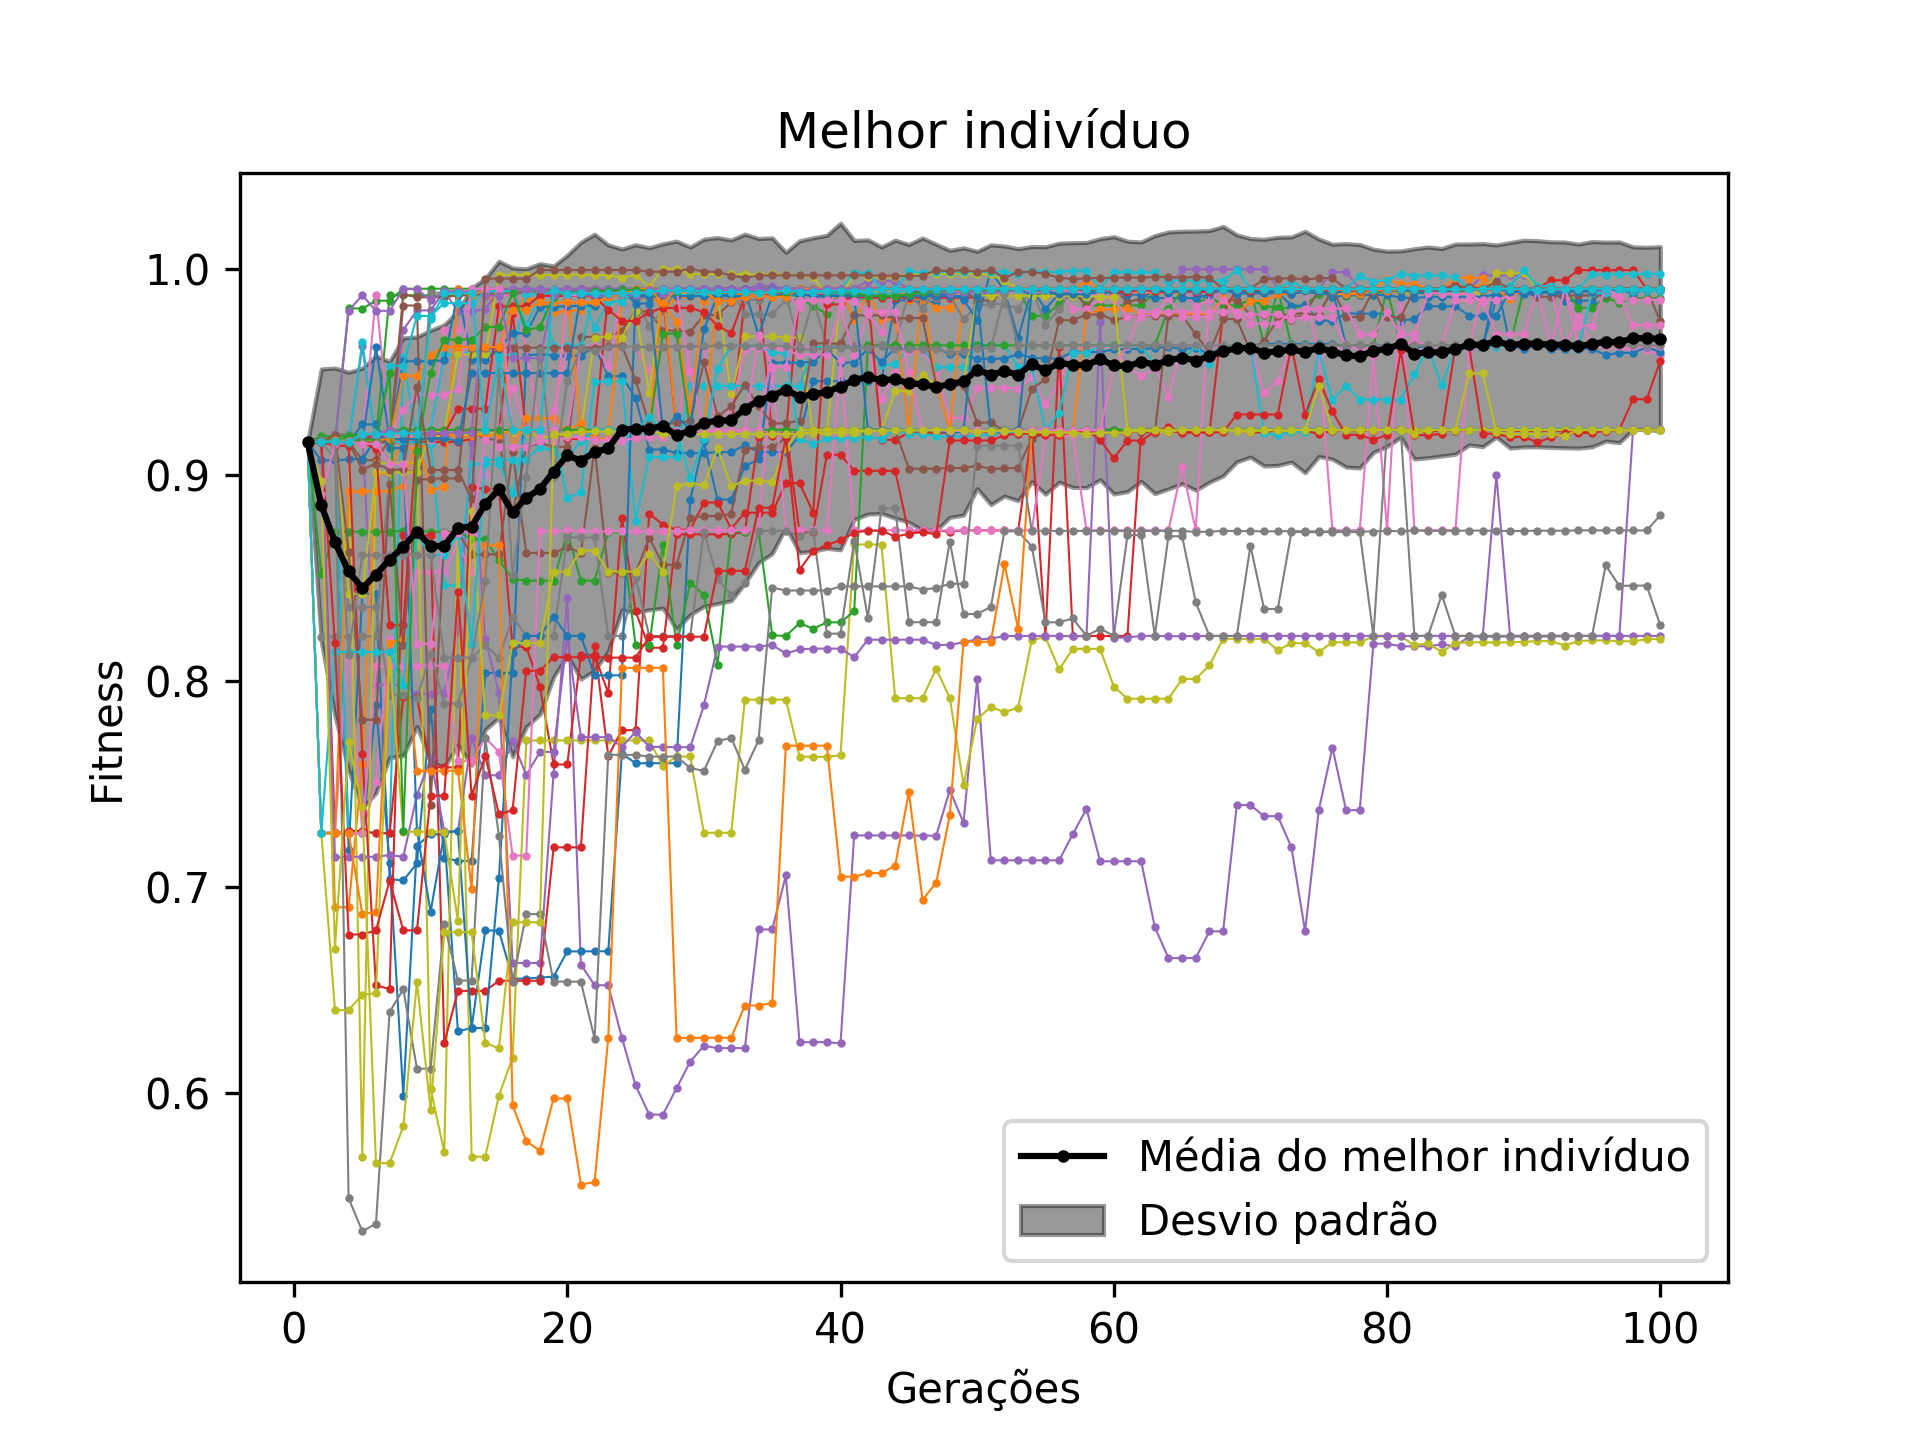
\includegraphics[width=1\textwidth]{sec-01/f6_none_fitness_vs_gen_best}
		\caption{Melhores indíviduos de todos os experimentos ao longo das gerações.
		Em preto é mostrado o comportamento médio dos 50 experimentos. }
	\end{subfigure}
	\hfill
	\begin{subfigure}{.45\textwidth}
		\centering
		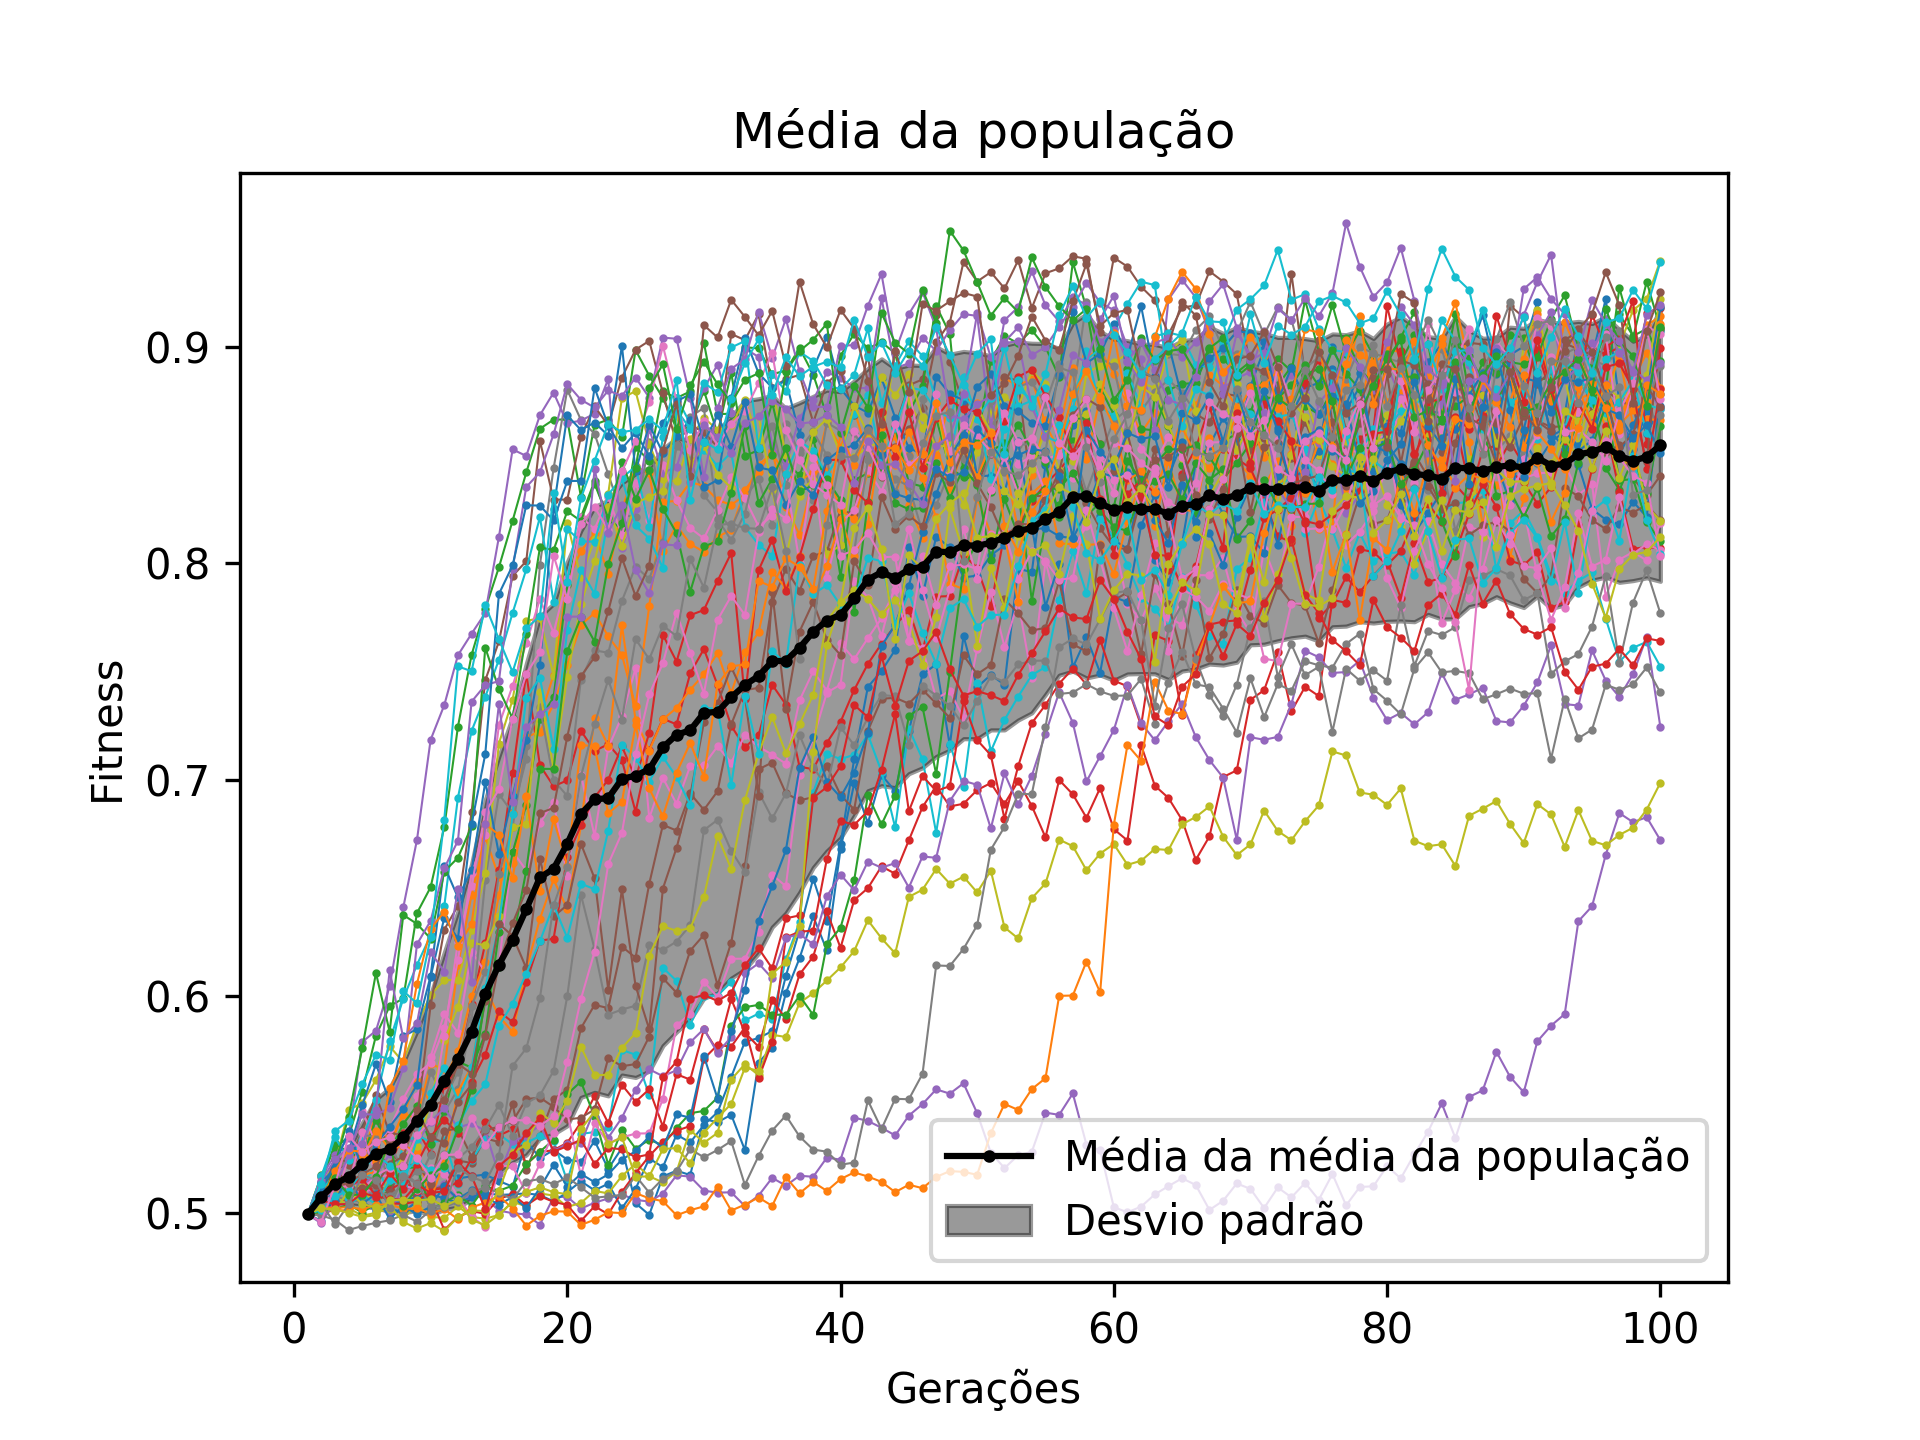
\includegraphics[width=1\textwidth]{sec-01/f6_none_fitness_vs_gen_pop}
		\caption{Média da população de todos os experimentos ao longo das gerações.
		Em preto é mostrado o comportamento médio dos 50 experimentos.}
	\end{subfigure}
	\caption{Resultados obtidos para a função $f6$ sem elitismo ou estado estacionário referentes ao teste 3 da tabela~\ref{tab:f6_none}}
\end{figure}

\begin{figure}[!htb]
	\begin{subfigure}{.45\textwidth}
		\centering
		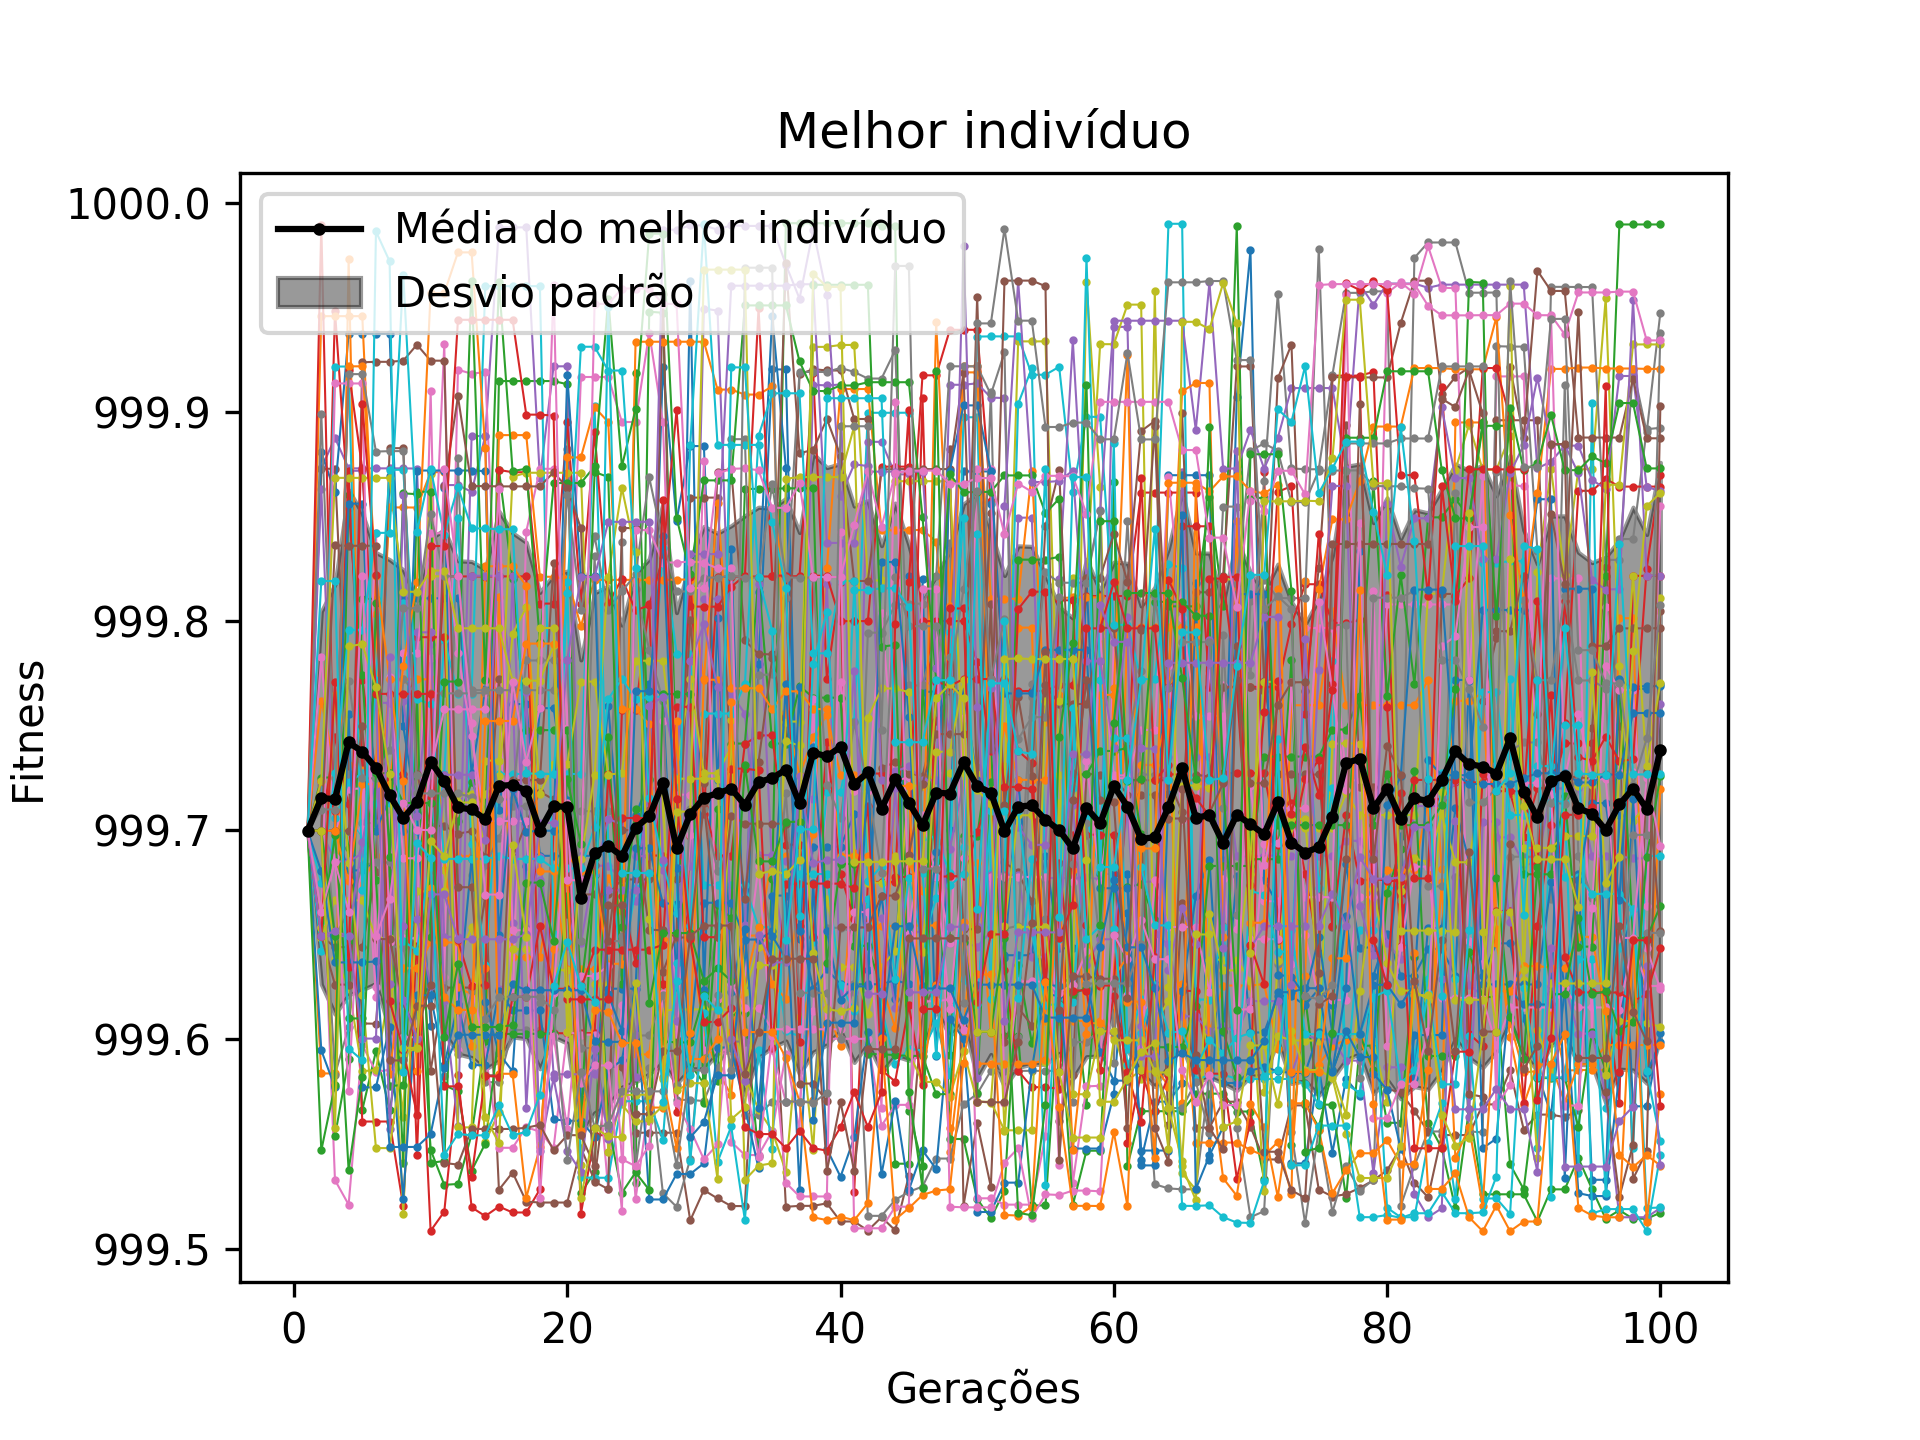
\includegraphics[width=1\textwidth]{sec-01/f6e_none_fitness_vs_gen_best}
		\caption{Melhores indíviduos de todos os experimentos ao longo das gerações.
		Em preto é mostrado o comportamento médio dos 50 experimentos. }
	\end{subfigure}
	\hfill
	\begin{subfigure}{.45\textwidth}
		\centering
		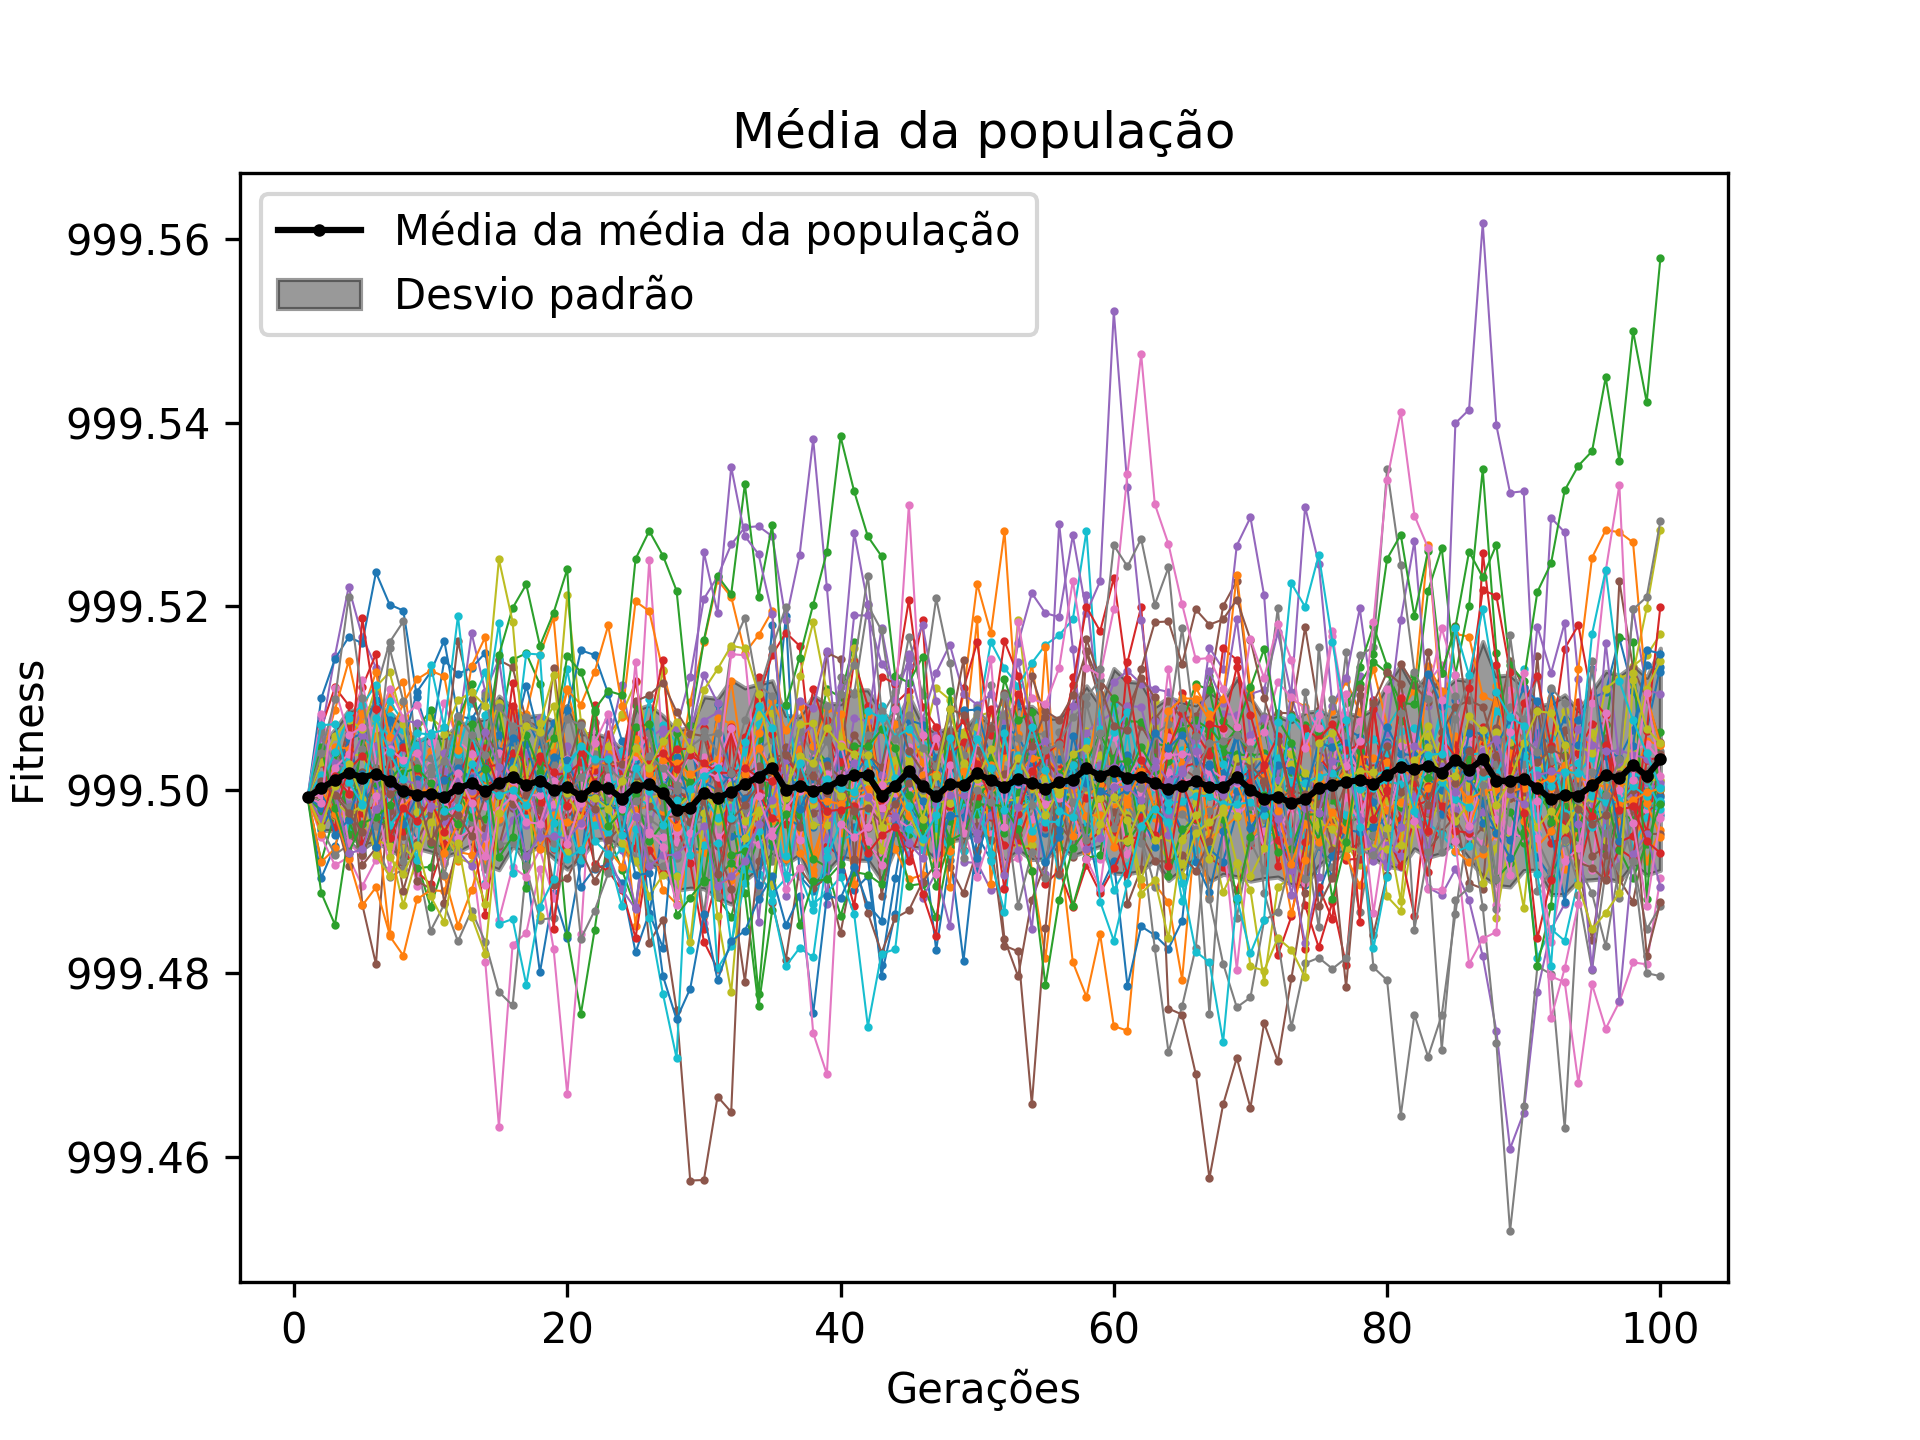
\includegraphics[width=1\textwidth]{sec-01/f6e_none_fitness_vs_gen_pop}
		\caption{Média da população de todos os experimentos ao longo das gerações.
		Em preto é mostrado o comportamento médio dos 50 experimentos.}
	\end{subfigure}
	\caption{Resultados obtidos para a função $f6_{elevada}$ sem elitismo ou estado estacionário referentes ao teste 1 da tabela~\ref{tab:f6_none}}
\end{figure}

\begin{figure}[!htb]
	\begin{subfigure}{.45\textwidth}
		\centering
		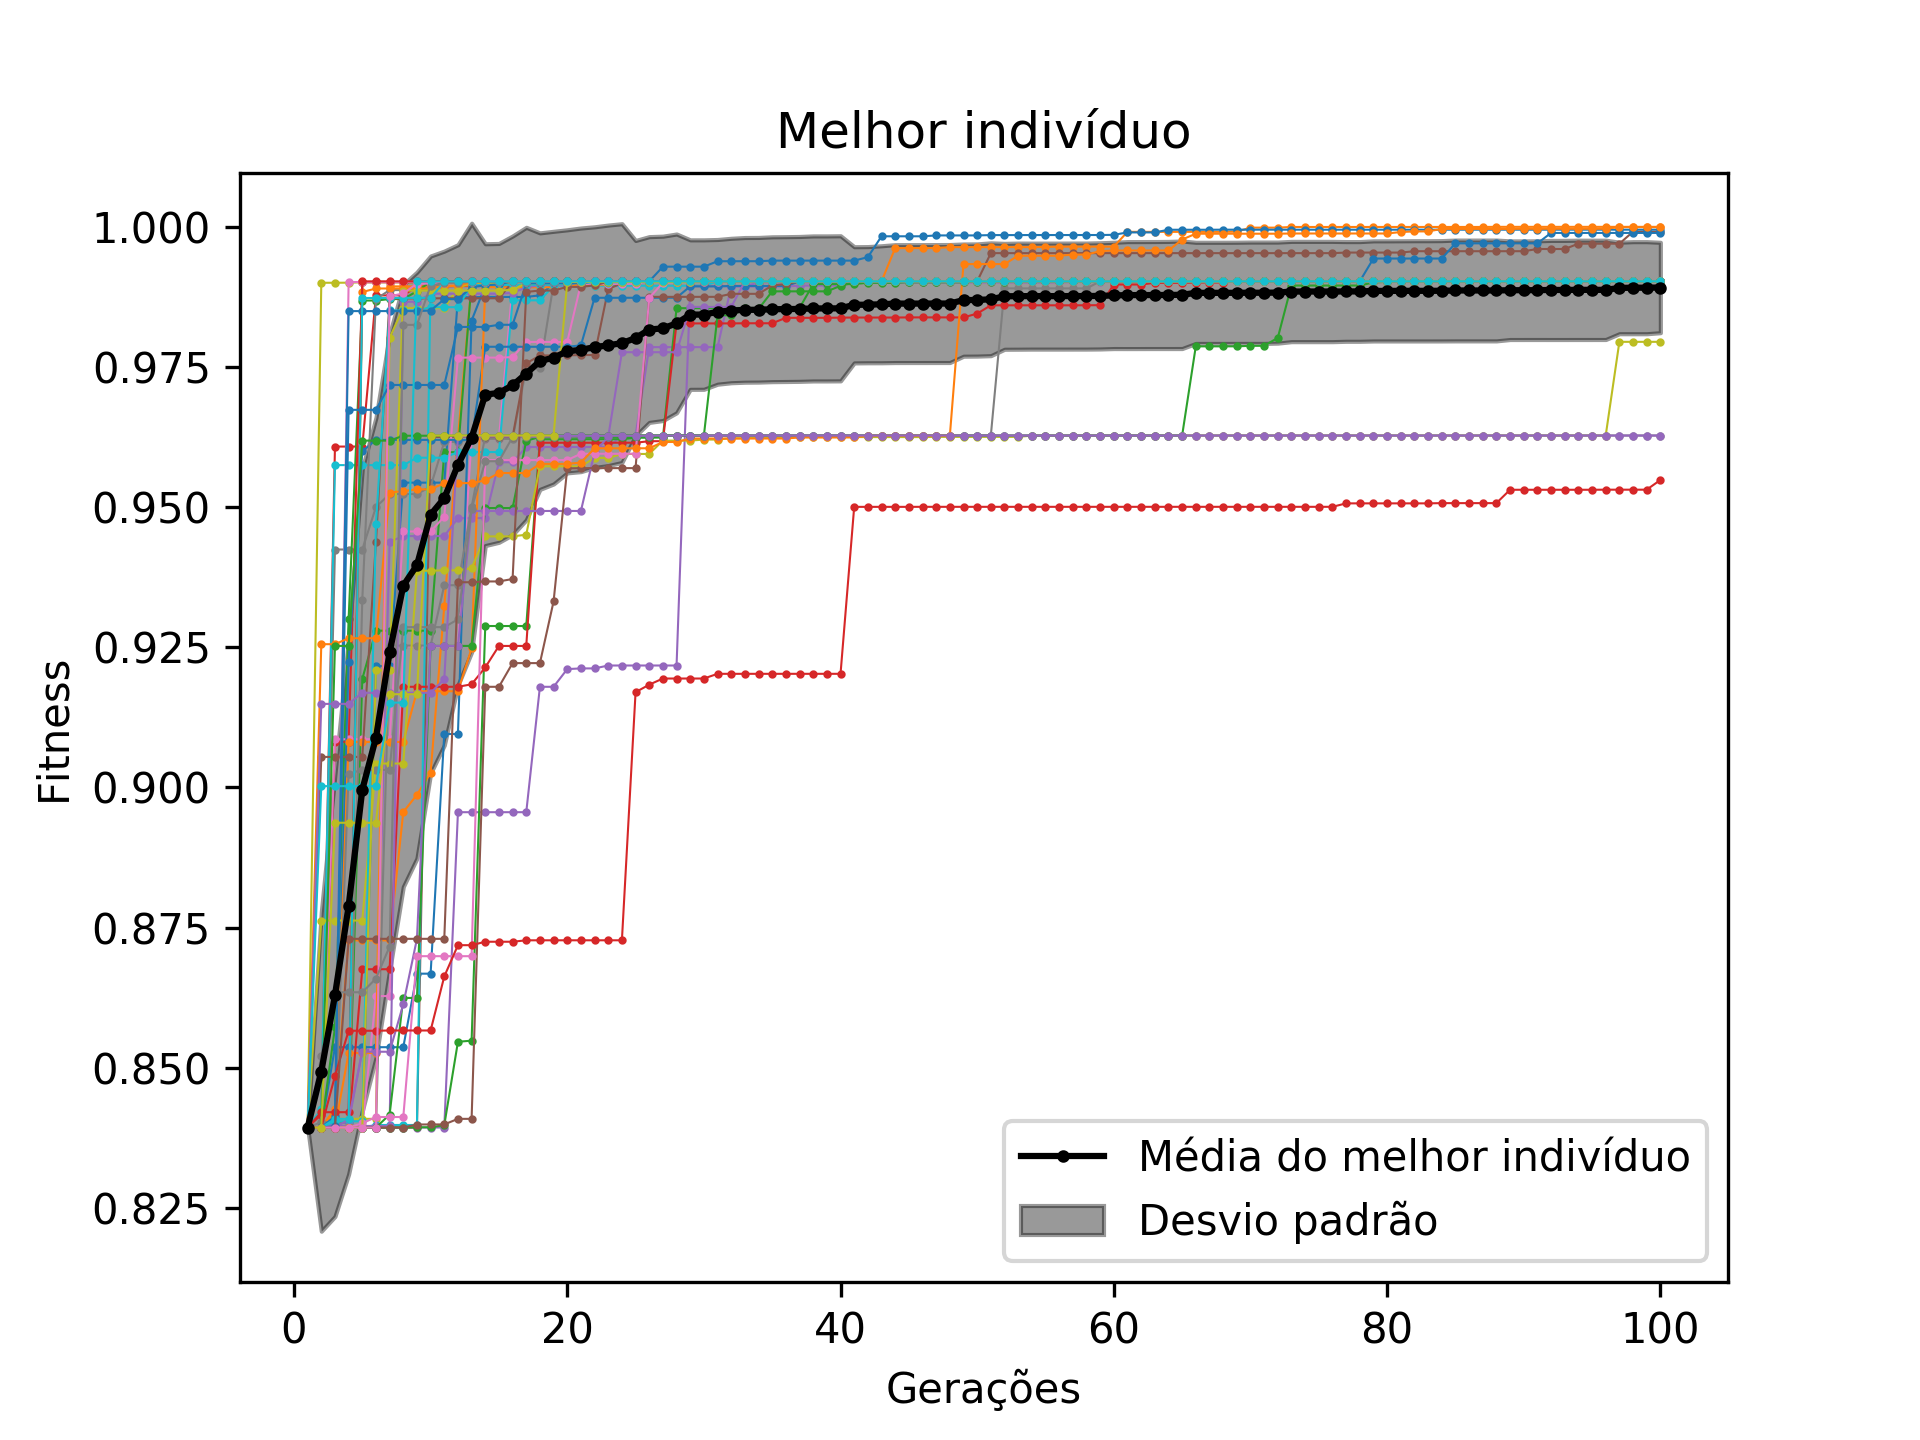
\includegraphics[width=1\textwidth]{sec-01/f6_elitist_fitness_vs_gen_best}
		\caption{Melhores indíviduos de todos os experimentos ao longo das gerações.
		Em preto é mostrado o comportamento médio dos 50 experimentos. }
	\end{subfigure}
	\hfill
	\begin{subfigure}{.45\textwidth}
		\centering
		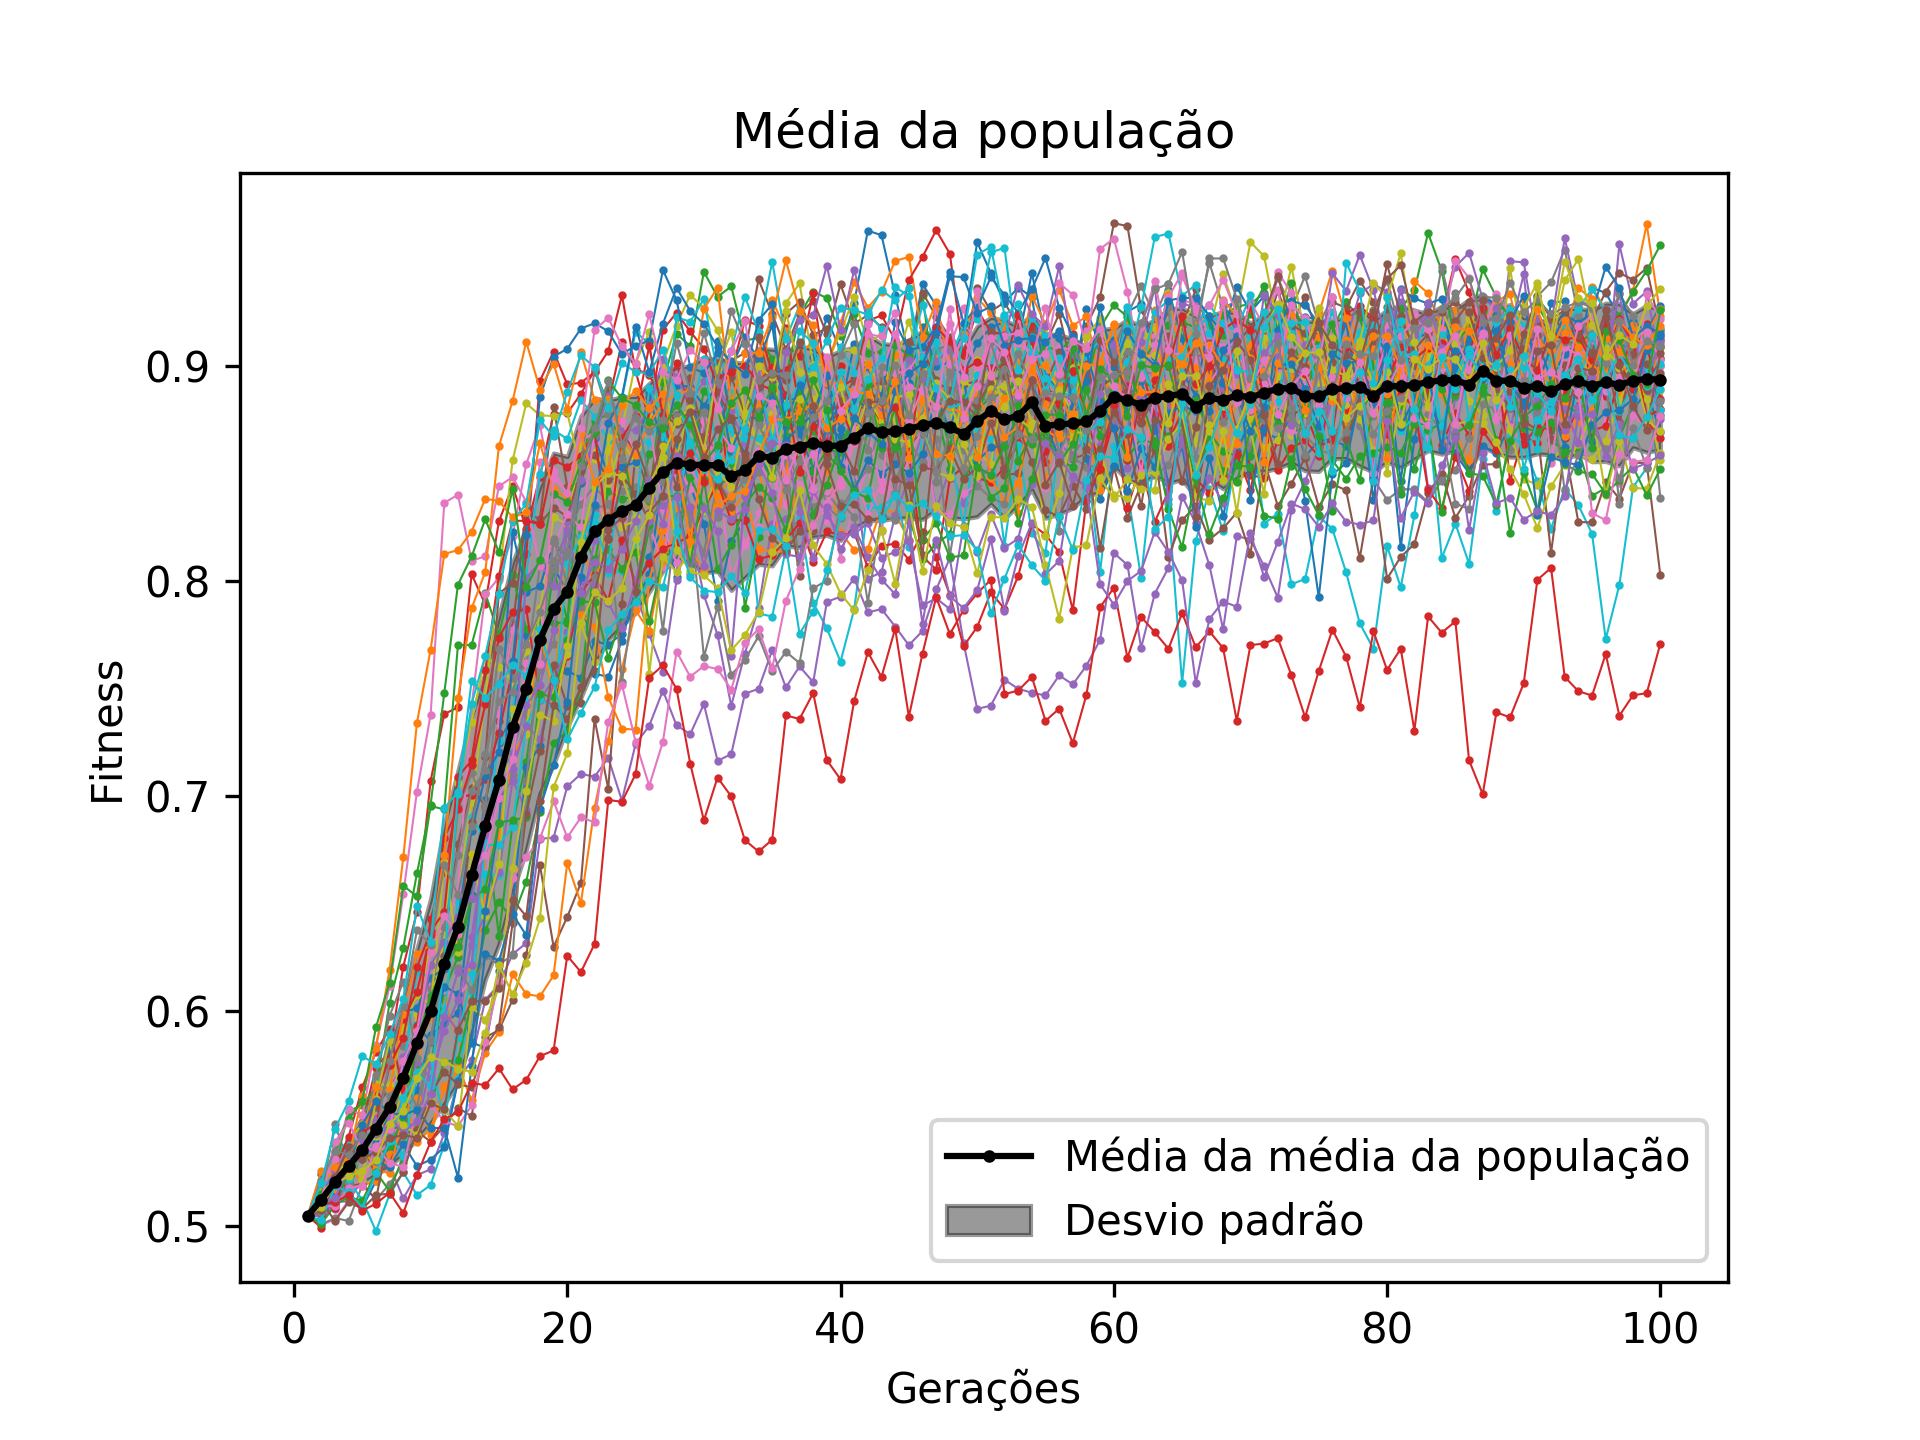
\includegraphics[width=1\textwidth]{sec-01/f6_elitist_fitness_vs_gen_pop}
		\caption{Média da população de todos os experimentos ao longo das gerações.
		Em preto é mostrado o comportamento médio dos 50 experimentos.}
	\end{subfigure}
	\caption{Resultados obtidos para a função $f6$ com elitismo referentes ao teste 5 da tabela~\ref{tab:f6_elitist}}
\end{figure}

\begin{figure}[!htb]
	\begin{subfigure}{.45\textwidth}
		\centering
		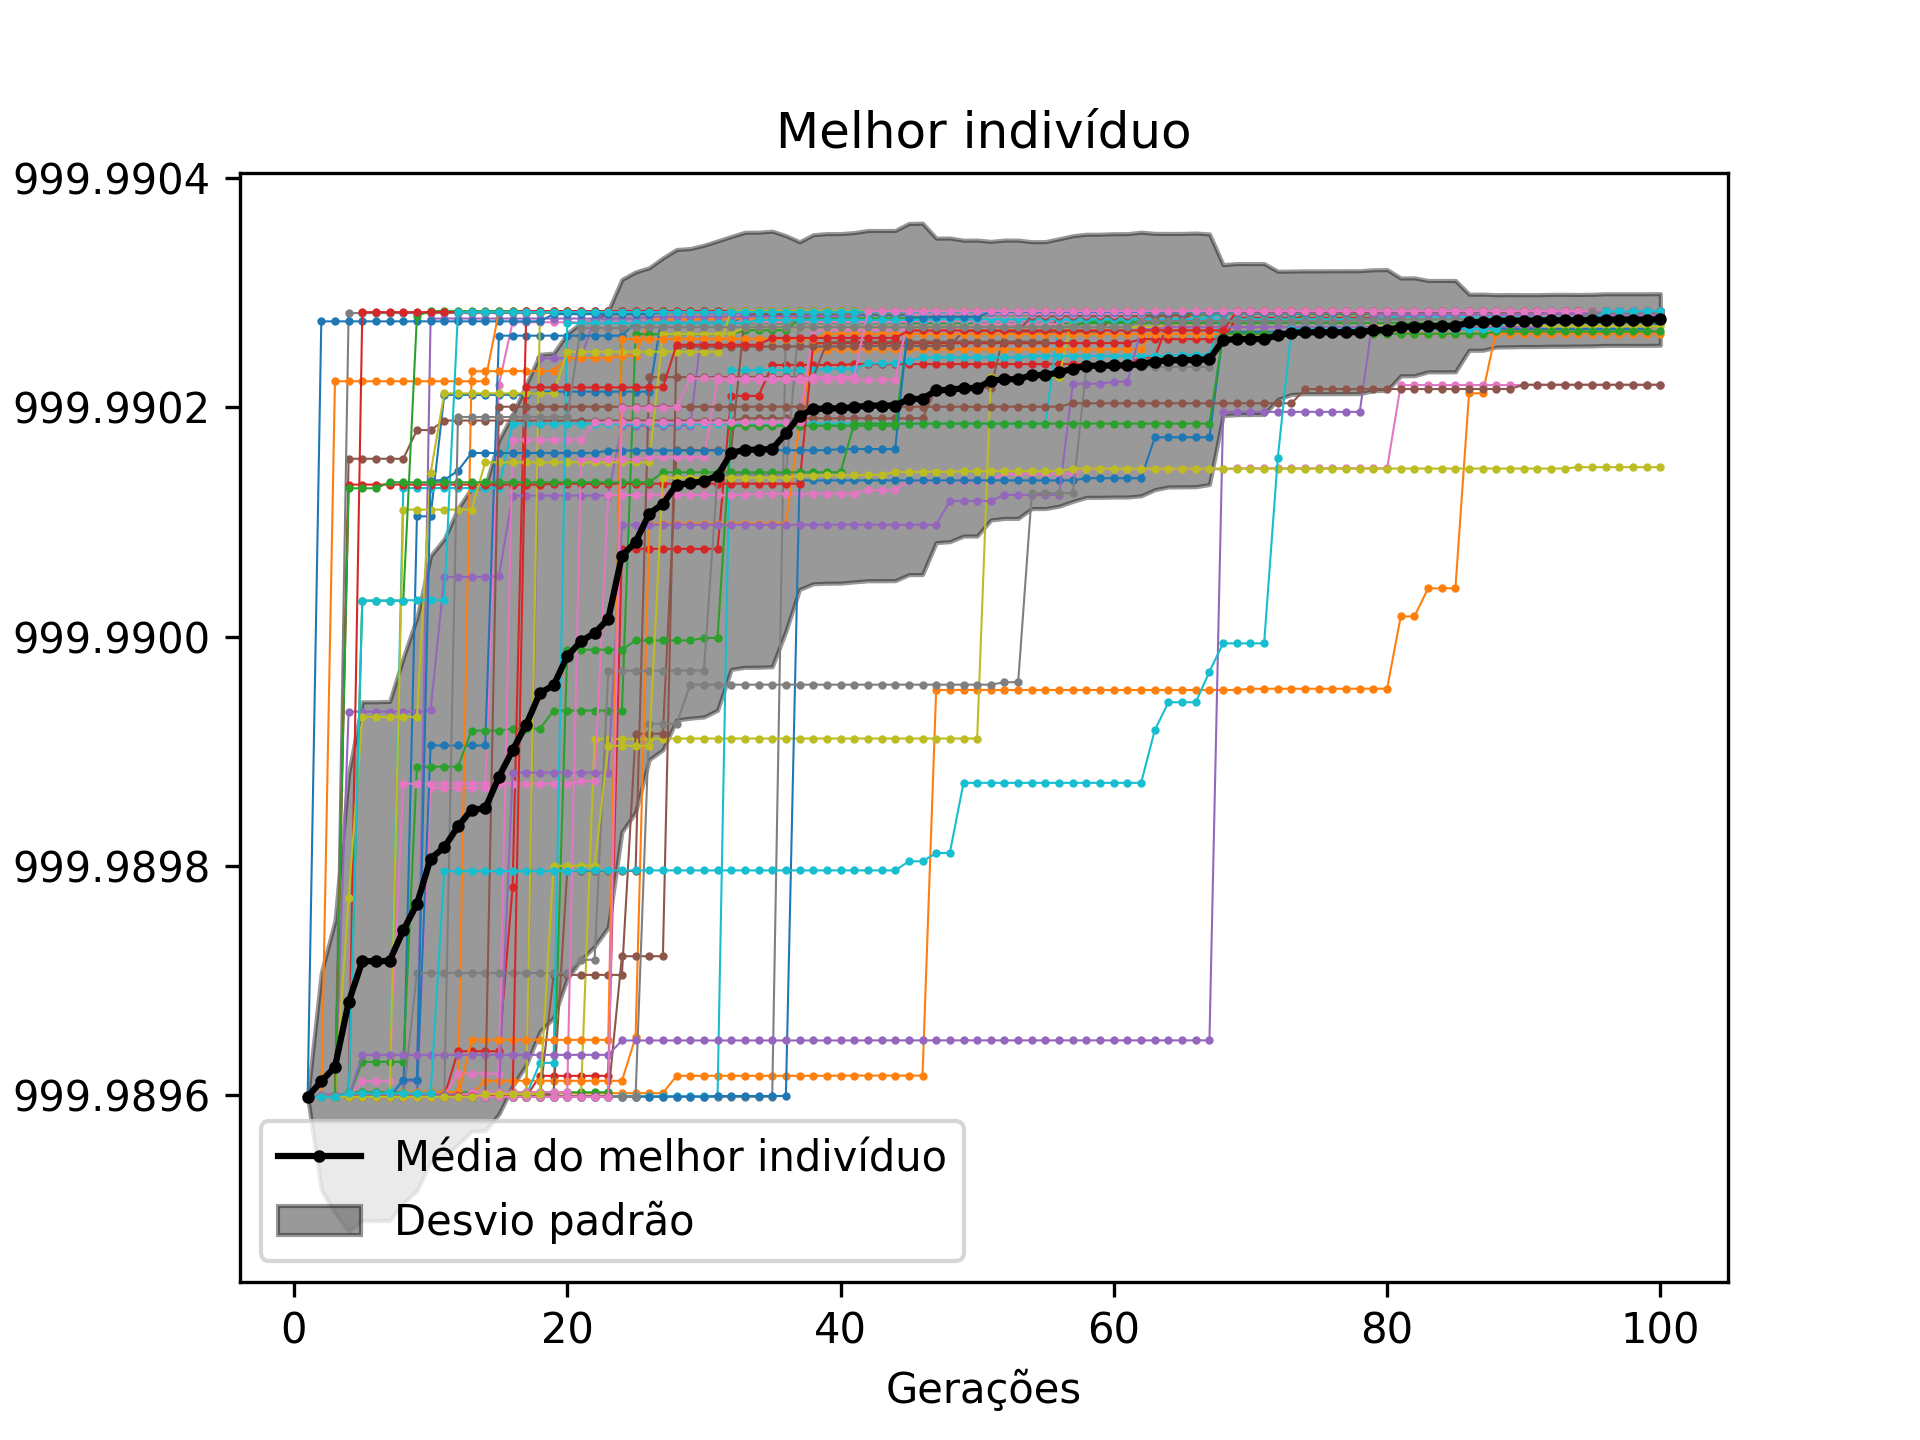
\includegraphics[width=1\textwidth]{sec-01/f6e_elitist_fitness_vs_gen_best}
		\caption{Melhores indíviduos de todos os experimentos ao longo das gerações.
		Em preto é mostrado o comportamento médio dos 50 experimentos. }
	\end{subfigure}
	\hfill
	\begin{subfigure}{.45\textwidth}
		\centering
		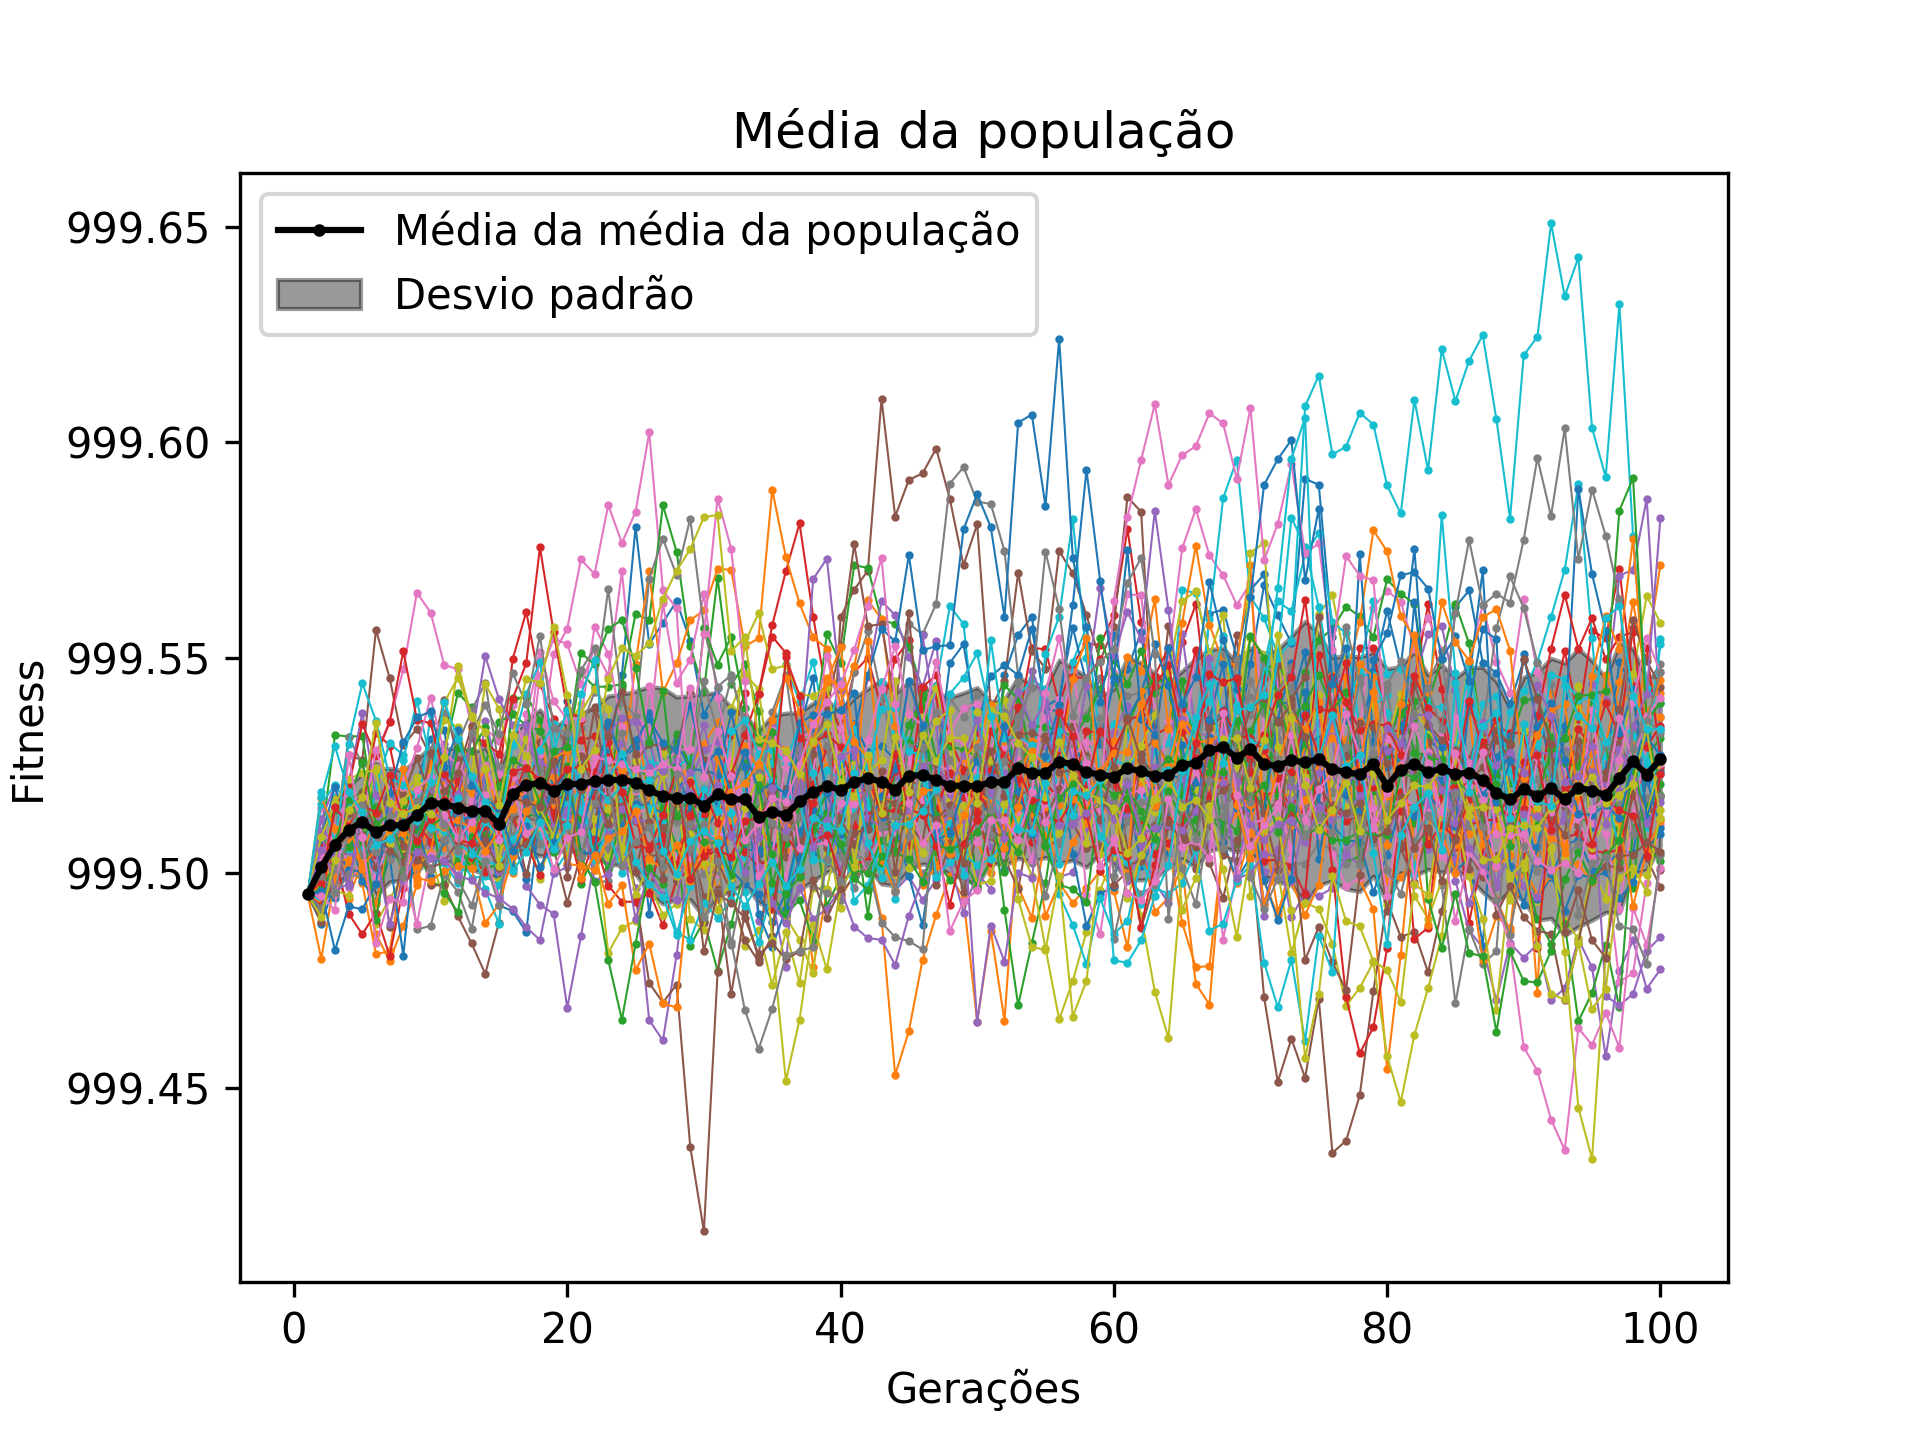
\includegraphics[width=1\textwidth]{sec-01/f6e_elitist_fitness_vs_gen_pop}
		\caption{Média da população de todos os experimentos ao longo das gerações.
		Em preto é mostrado o comportamento médio dos 50 experimentos.}
	\end{subfigure}
	\caption{Resultados obtidos para a função $f6_{elevada}$ com elitismo referentes ao teste 3 da tabela~\ref{tab:f6_elitist}}
\end{figure}

	Posteriormente, utilizando a elitismo e estado estacionário obtiveram-se um aumento de performance tanto para a função
	$f6$ quanto para a função $f6_{elevada}$. Os resultados obtidos são apresentados nas tabelas~\ref{tab:f6_elitist}
	e \ref{tab:f6_stationary}.

	\begin{table}[!htb]
		\centering
		\begin{tabular}{|c|c|c|c|c|}
			\hline
			\rowcolor[HTML]{9B9B9B}
			& \multicolumn{2}{c}{Função F6} & \multicolumn{2}{c}{Função F6 elevada} \\
			\rowcolor[HTML]{9B9B9B}
			Teste & Média melhor indíviduo & Média população & Média melhor indíviduo & Média população \\\hline
			1 & 0.98518 & 0.88408 & 999.99028 & 999.52910 \\\hline
			2 & 0.97977 & 0.87092 & 999.98128 & 999.52672 \\\hline
			3 & 0.97706 & 0.86914 & 999.98433 & 999.53551 \\\hline
			4 & 0.97921 & 0.87249 & 999.98058 & 999.52753 \\\hline
			5 & 0.98918 & 0.89792 & 999.98472 & 999.52755 \\\hline
			\textbf{Média Final} & \textbf{0.98208} & \textbf{0.87891} & \textbf{999.98424} & \textbf{999.5293} \\\hline
		\end{tabular}
		\caption{Resultados da função $f6$ e $f6_{elevada}$ com elitismo. \label{tab:f6_elitist}}
	\end{table}

	\begin{table}[!htb]
		\centering
		\begin{tabular}{|c|c|c|c|c|}
			\hline
			\rowcolor[HTML]{9B9B9B}
			& \multicolumn{2}{c}{Função F6} & \multicolumn{2}{c}{Função F6 elevada} \\
			\rowcolor[HTML]{9B9B9B}
			Teste & Média melhor indíviduo & Média população & Média melhor indíviduo & Média população \\\hline
			1 & 0.96897 & 0.95154 & 999.98164 & 999.96859 \\\hline
			2 & 0.96789 & 0.95841 & 999.95580 & 999.93493 \\\hline
			3 & 0.97028 & 0.95798 & 999.96191 & 999.94779 \\\hline
			4 & 0.98858 & 0.98103 & 999.98187 & 999.96661 \\\hline
			5 & 0.96920 & 0.95792 & 999.97647 & 999.95859 \\\hline
			\textbf{Média Final} & \textbf{0.97298} & \textbf{0.96138} & \textbf{999.97154} & \textbf{999.95530} \\\hline
		\end{tabular}
		\caption{Resultados da função $f6$ e $f6_{elevada}$ com estado estacionário de 20\% \label{tab:f6_stationary}}
	\end{table}

	\begin{figure}[!htb]
		\begin{subfigure}{.45\textwidth}
			\centering
			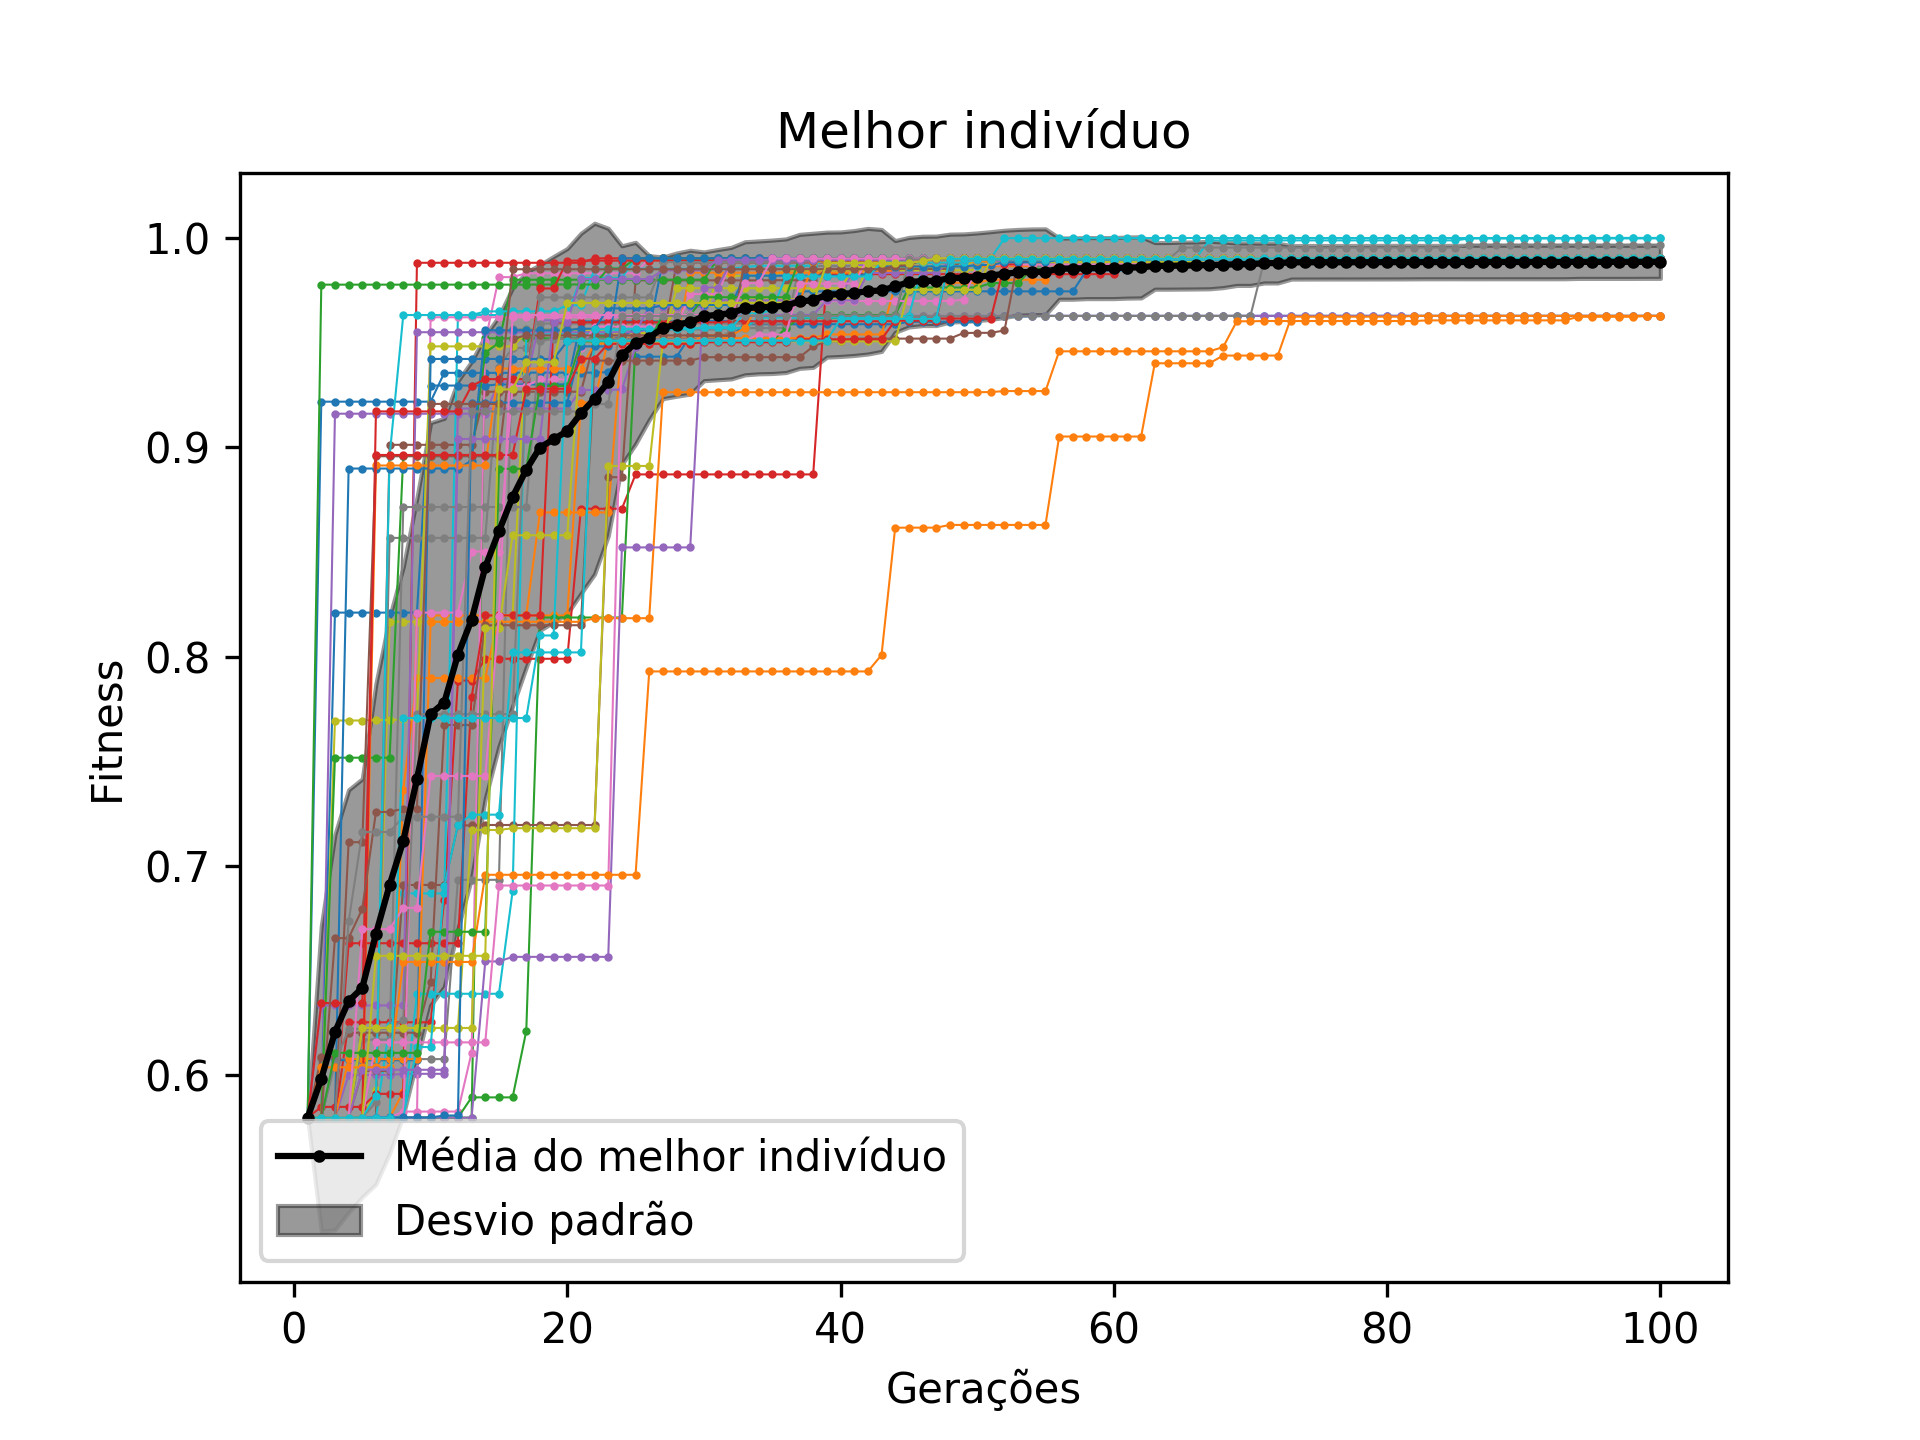
\includegraphics[width=1\textwidth]{sec-01/f6_ss_fitness_vs_gen_best}
			\caption{Melhores indíviduos de todos os experimentos ao longo das gerações.
			Em preto é mostrado o comportamento médio dos 50 experimentos. }
		\end{subfigure}
		\hfill
		\begin{subfigure}{.45\textwidth}
			\centering
			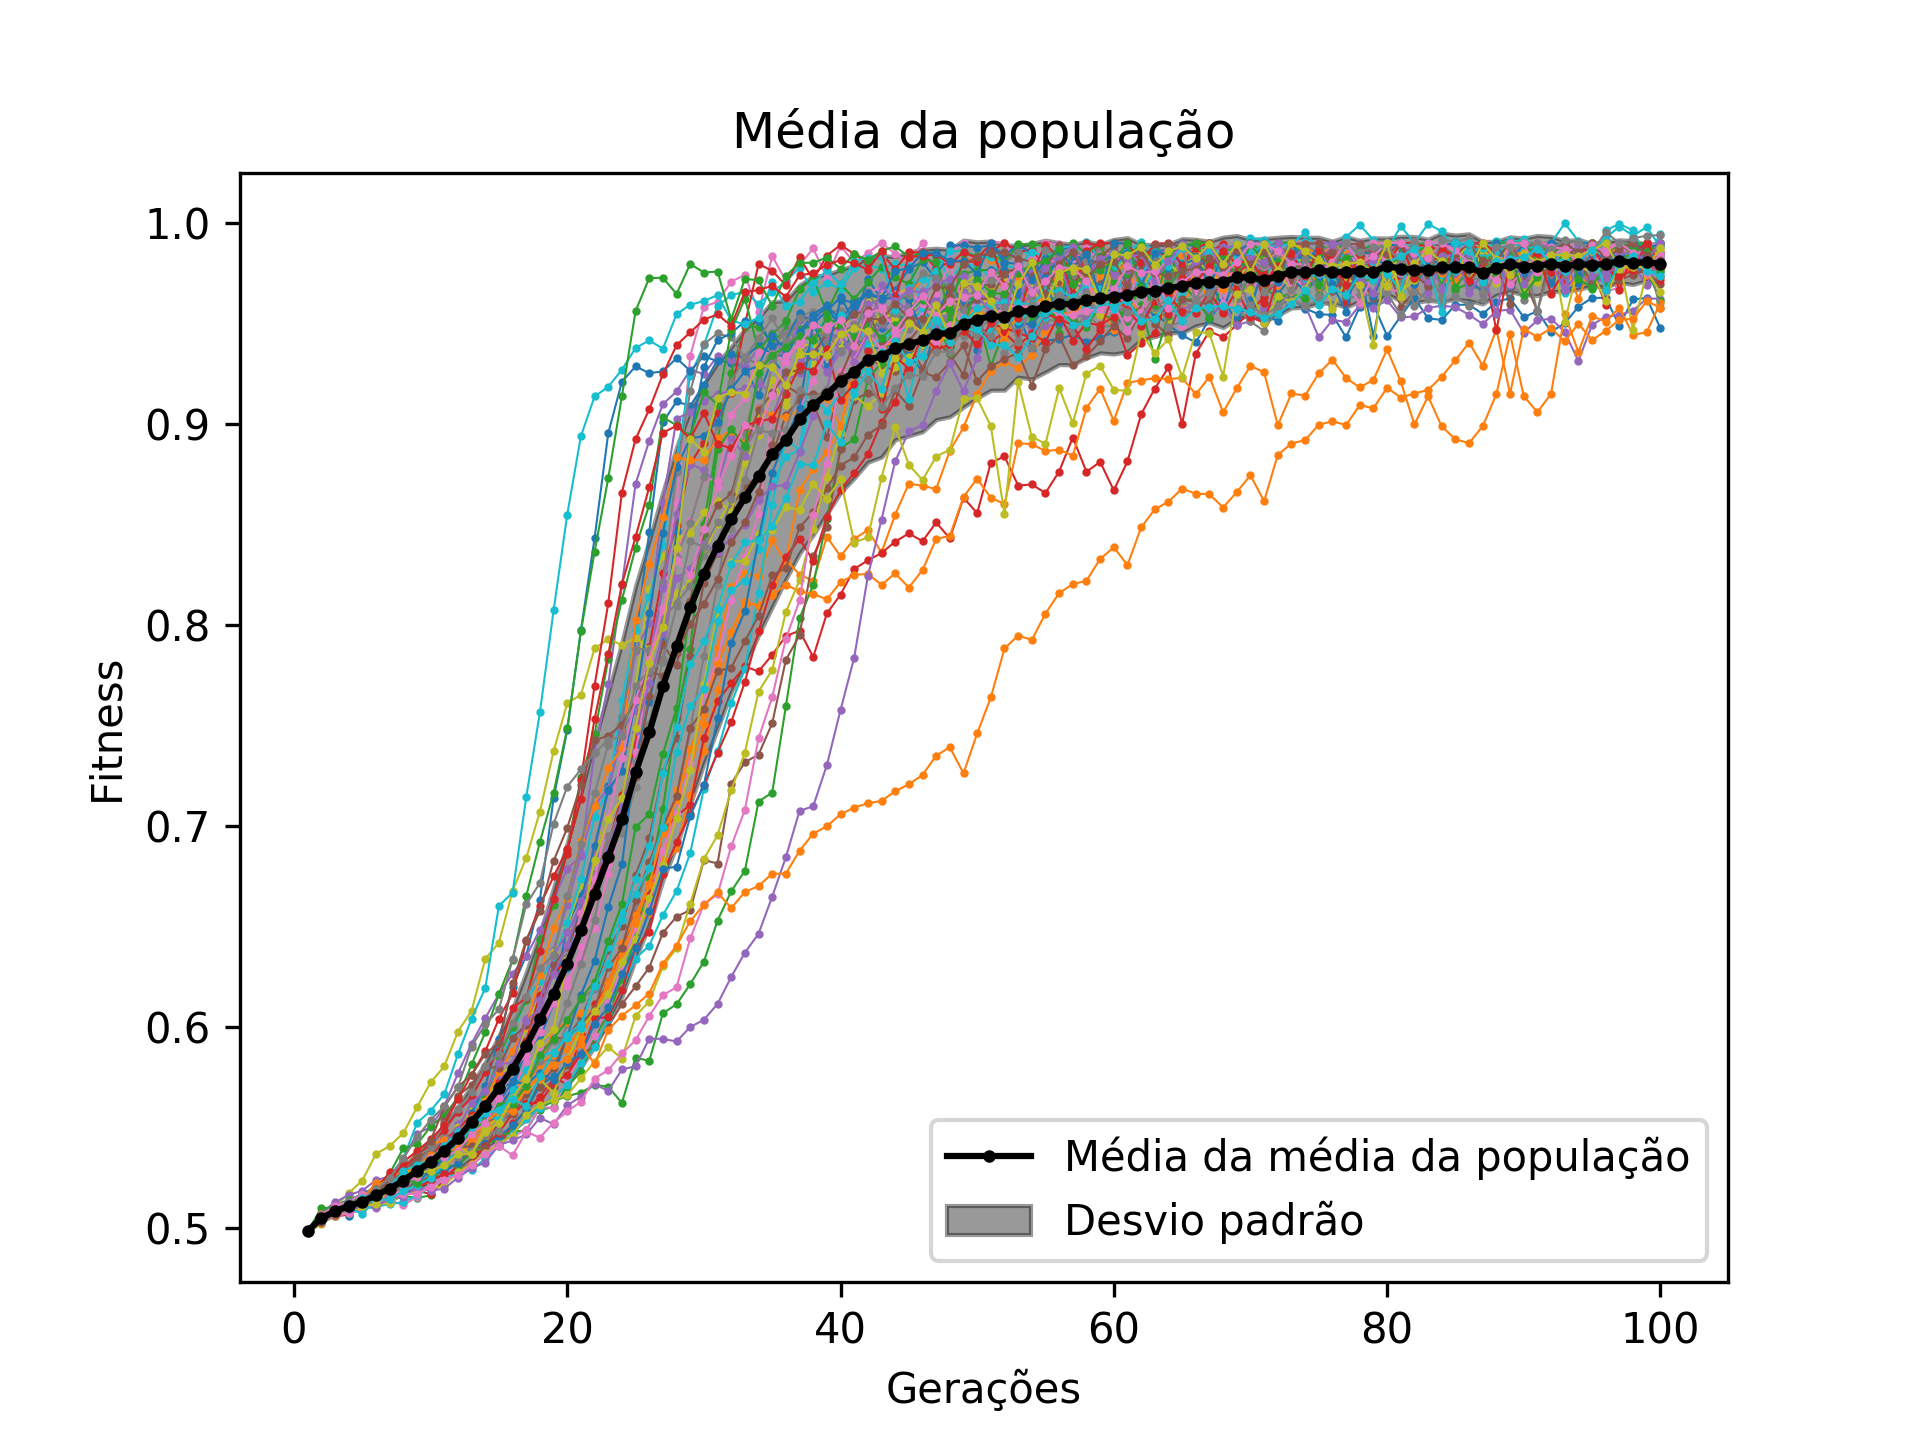
\includegraphics[width=1\textwidth]{sec-01/f6_ss_fitness_vs_gen_pop}
			\caption{Média da população de todos os experimentos ao longo das gerações.
			Em preto é mostrado o comportamento médio dos 50 experimentos.}
		\end{subfigure}
		\caption{Resultados obtidos para a função $f6$ com estado estacionário de 20\% referentes ao teste 4 da tabela~\ref{tab:f6_stationary}}
	\end{figure}

	\begin{figure}[!htb]
		\begin{subfigure}{.45\textwidth}
			\centering
			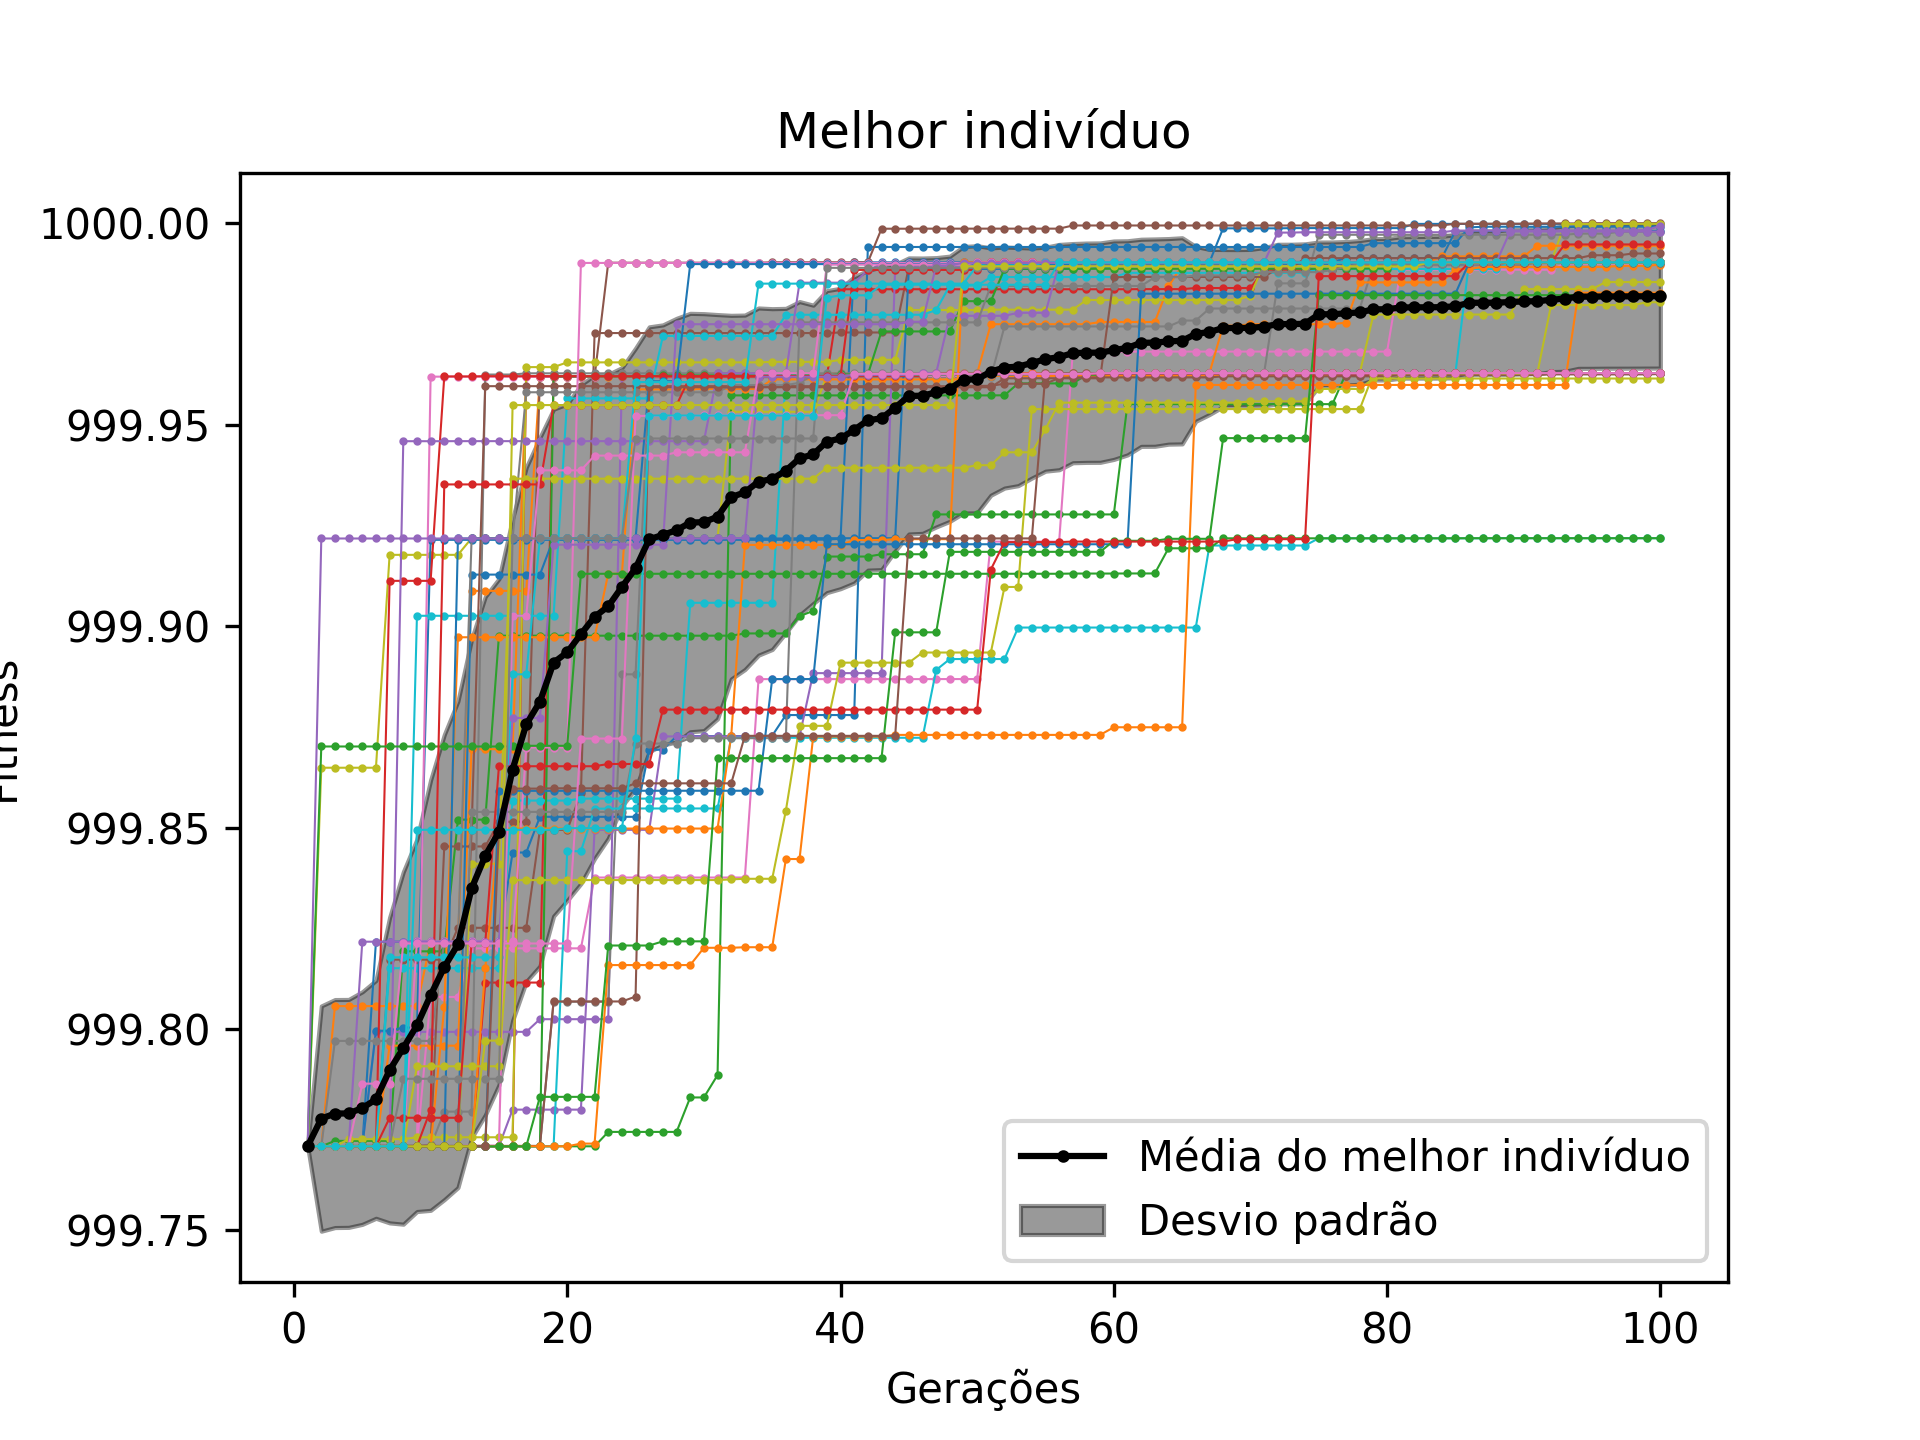
\includegraphics[width=1\textwidth]{sec-01/f6e_ss_fitness_vs_gen_best}
			\caption{Melhores indíviduos de todos os experimentos ao longo das gerações.
			Em preto é mostrado o comportamento médio dos 50 experimentos. }
		\end{subfigure}
		\hfill
		\begin{subfigure}{.45\textwidth}
			\centering
			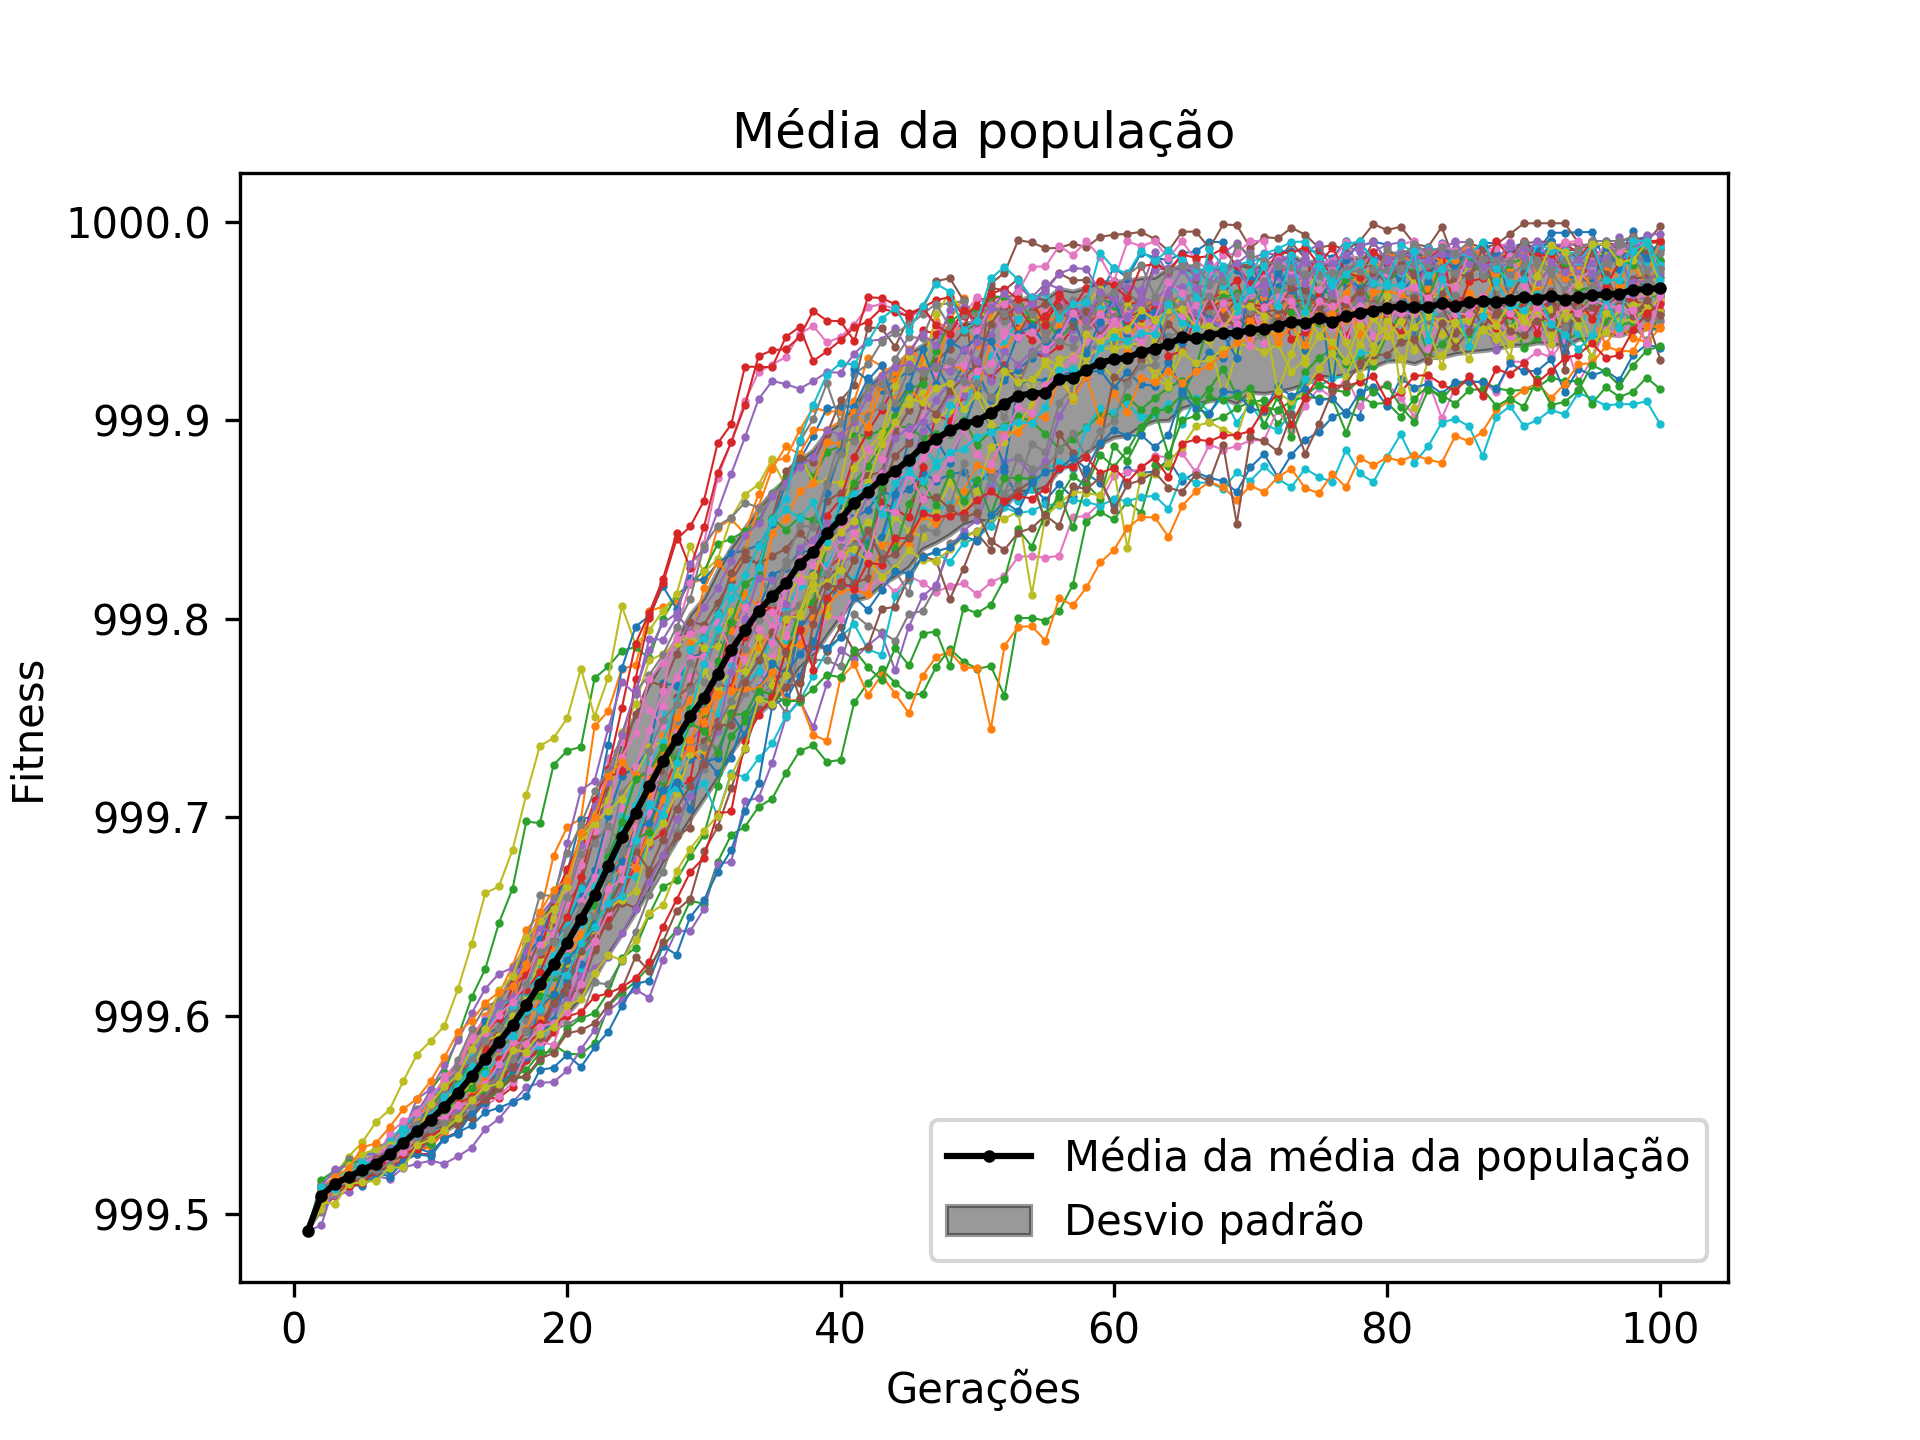
\includegraphics[width=1\textwidth]{sec-01/f6e_ss_fitness_vs_gen_pop}
			\caption{Média da população de todos os experimentos ao longo das gerações.
			Em preto é mostrado o comportamento médio dos 50 experimentos.}
		\end{subfigure}
		\caption{Resultados obtidos para a função $f6_{elevada}$ com estado estacionário de 20\% referentes ao teste 4 da tabela~\ref{tab:f6_stationary}}
	\end{figure}

	\clearpage
	\section{Cruzamentos binário}
		Para comparar o impacto da performance de diferentes tipos de cruzamentos na função $f6$,
foram obtidos os resultados apresentados na tabela \ref{tab:f6_crux} utilizando, cruzamento de um ponto,
de dois pontos, de 10 pontos e cruzamento uniforme. A representação, seleção, operadores genéticos
e critério de paragem utilizando foram os mesmos utilizados na seção 1.

\begin{table}[htb]
	\centering
	\begin{tabular}{|c|c|c|}
		\hline
		\rowcolor[HTML]{9B9B9B}
		Cruzamento & Média melhor indíviduo & Média população \\\hline
		1 ponto & 0.94532 & 0.81428 \\\hline
		2 pontos & 0.96801 & 0.79992 \\\hline
		10 pontos & 0.98094 & 0.73474 \\\hline
		Uniforme & 0.96441 & 0.85488 \\\hline
	\end{tabular}
	\caption{Resultados da função $f6$ utilizando vários tipos de cruzamentos \label{tab:f6_crux}}
\end{table}



\begin{figure}[htb]
	\begin{subfigure}{.45\textwidth}
		\centering
		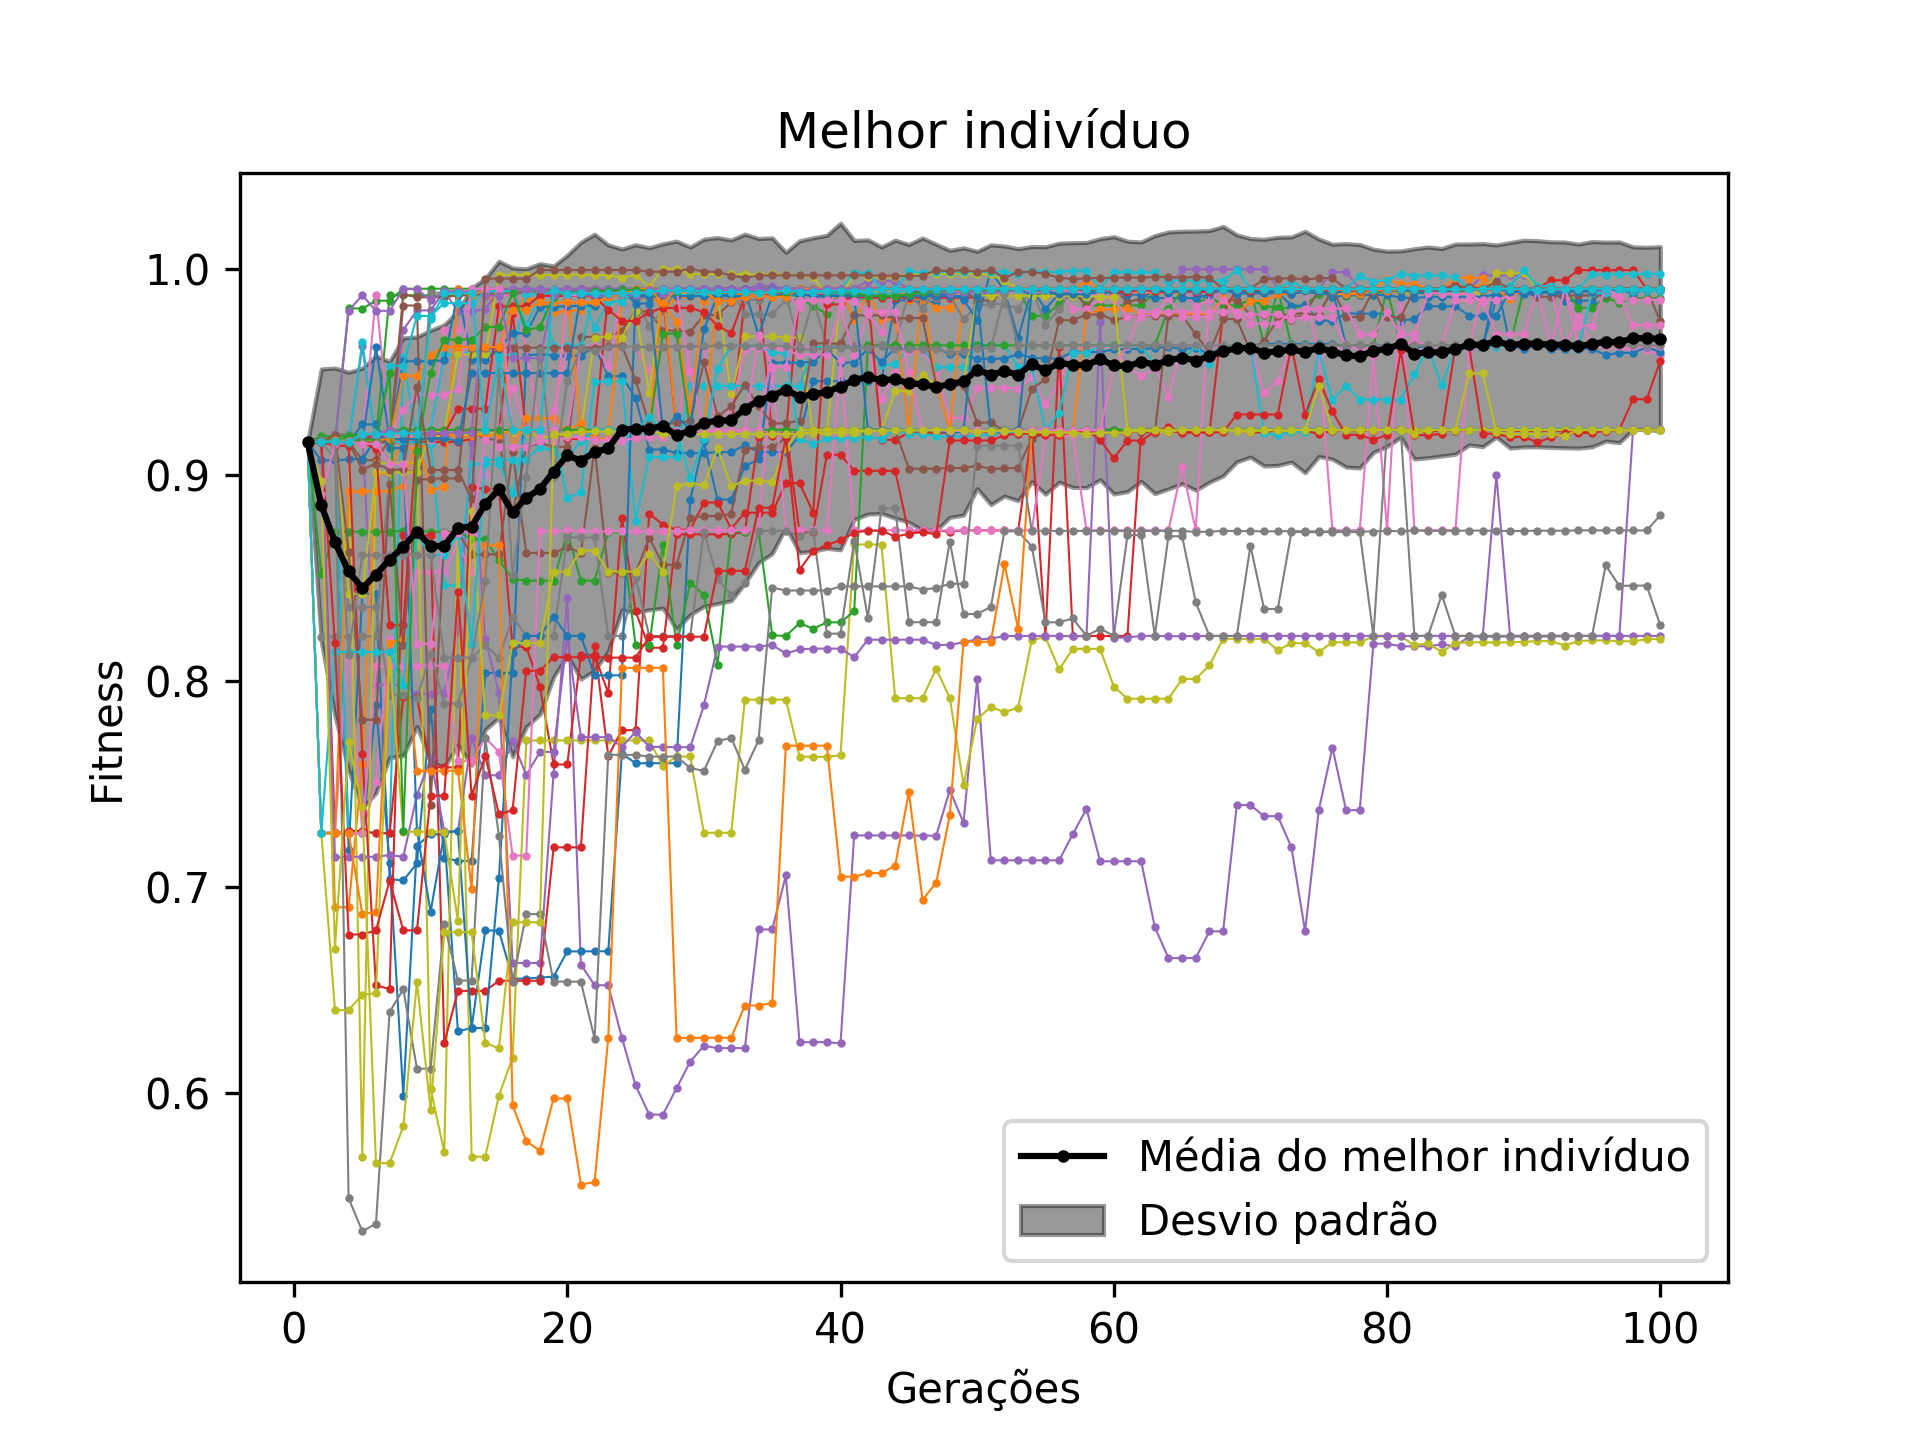
\includegraphics[width=1\textwidth]{sec-02/f6_1p_fitness_vs_gen_best.png}
		\caption{Melhores indíviduos de todos os experimentos ao longo das gerações.
		Em preto é mostrado o comportamento médio dos 50 experimentos. }
	\end{subfigure}
	\hfill
	\begin{subfigure}{.45\textwidth}
		\centering
		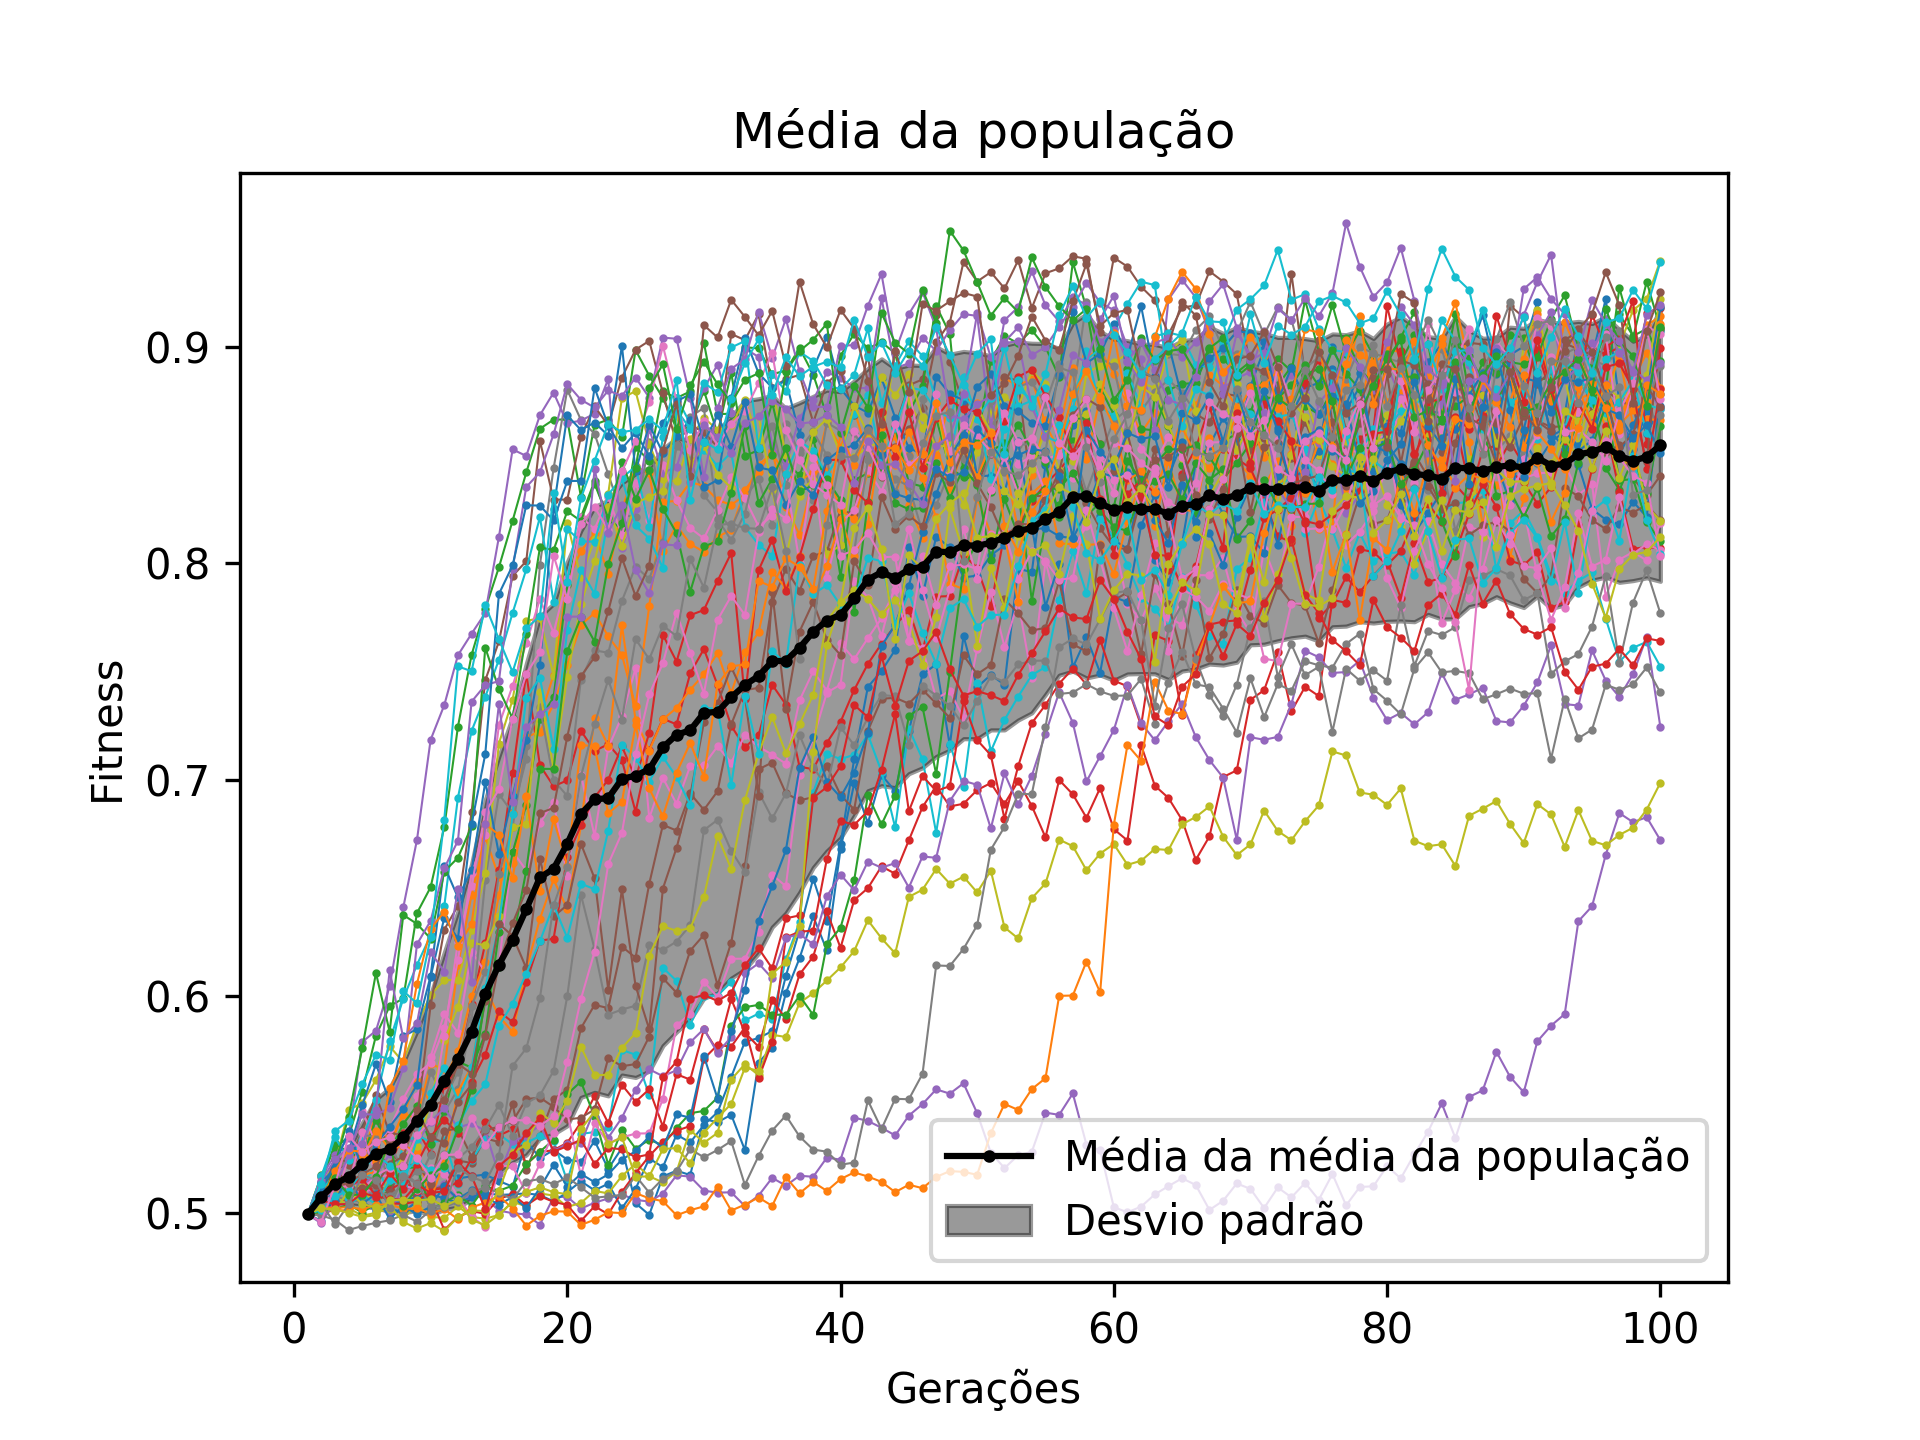
\includegraphics[width=1\textwidth]{sec-02/f6_1p_fitness_vs_gen_pop.png}
		\caption{Média da população de todos os experimentos ao longo das gerações.
		Em preto é mostrado o comportamento médio dos 50 experimentos.}
	\end{subfigure}
	\caption{Resultados obtidos para o caso de cruzamento de 1 ponto apresentado na tabela~\ref{tab:f6_crux}}
\end{figure}


	\begin{figure}[htb]
	\begin{subfigure}{.45\textwidth}
		\centering
		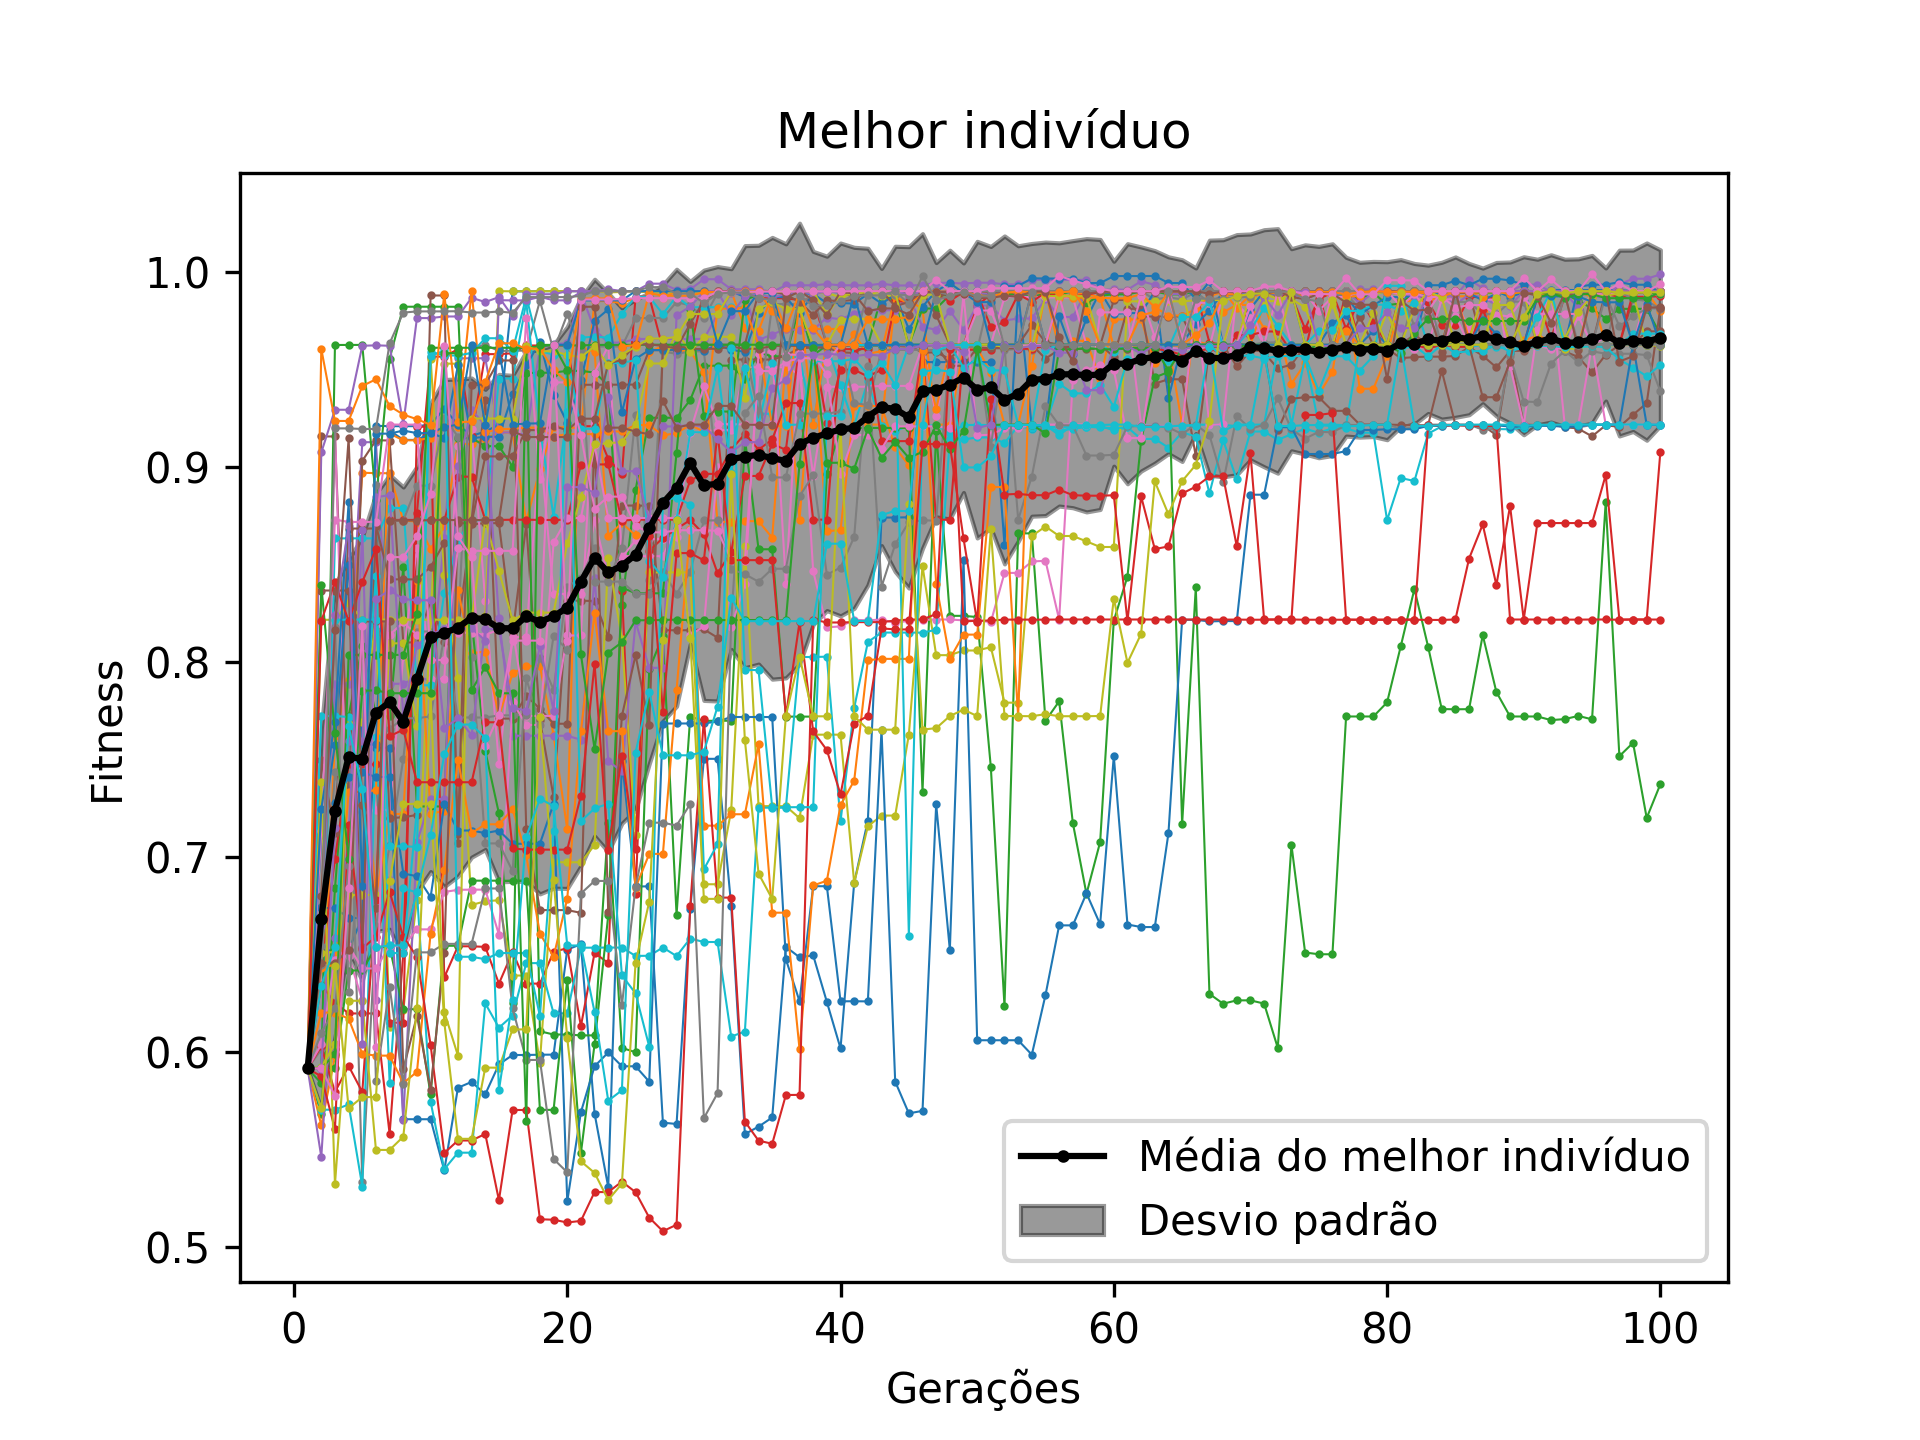
\includegraphics[width=1\textwidth]{sec-02/f6_2p_fitness_vs_gen_best.png}
		\caption{Melhores indíviduos de todos os experimentos ao longo das gerações.
		Em preto é mostrado o comportamento médio dos 50 experimentos. }
	\end{subfigure}
	\hfill
	\begin{subfigure}{.45\textwidth}
		\centering
		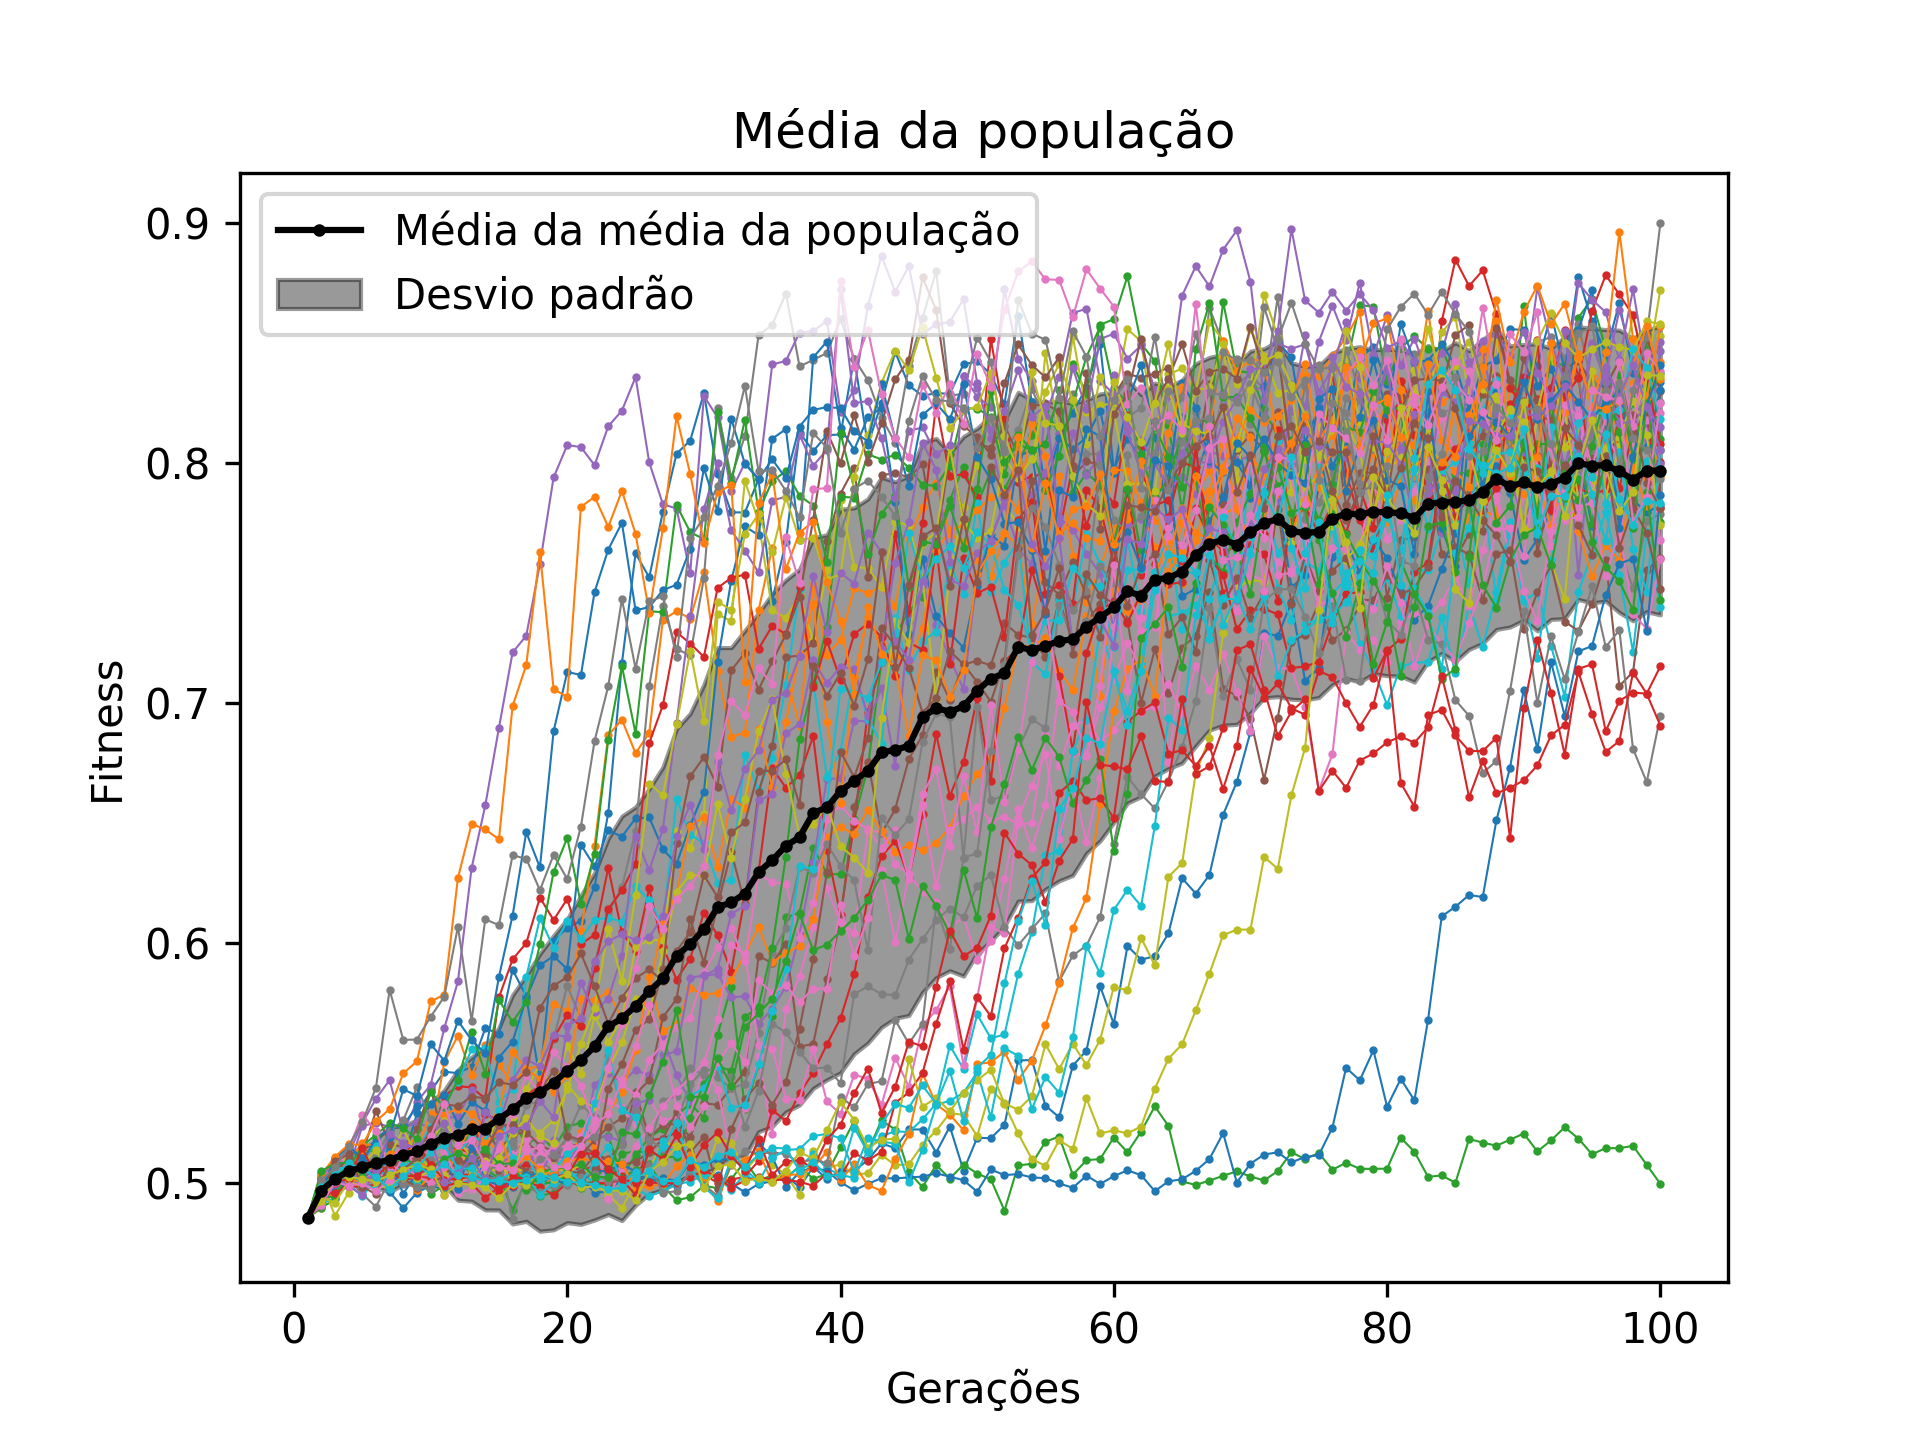
\includegraphics[width=1\textwidth]{sec-02/f6_2p_fitness_vs_gen_pop.png}
		\caption{Média da população de todos os experimentos ao longo das gerações.
		Em preto é mostrado o comportamento médio dos 50 experimentos.}
	\end{subfigure}
	\caption{Resultados obtidos para o caso de cruzamento de 2 pontos apresentado na tabela~\ref{tab:f6_crux}}
\end{figure}


	\begin{figure}[htb]
	\begin{subfigure}{.45\textwidth}
		\centering
		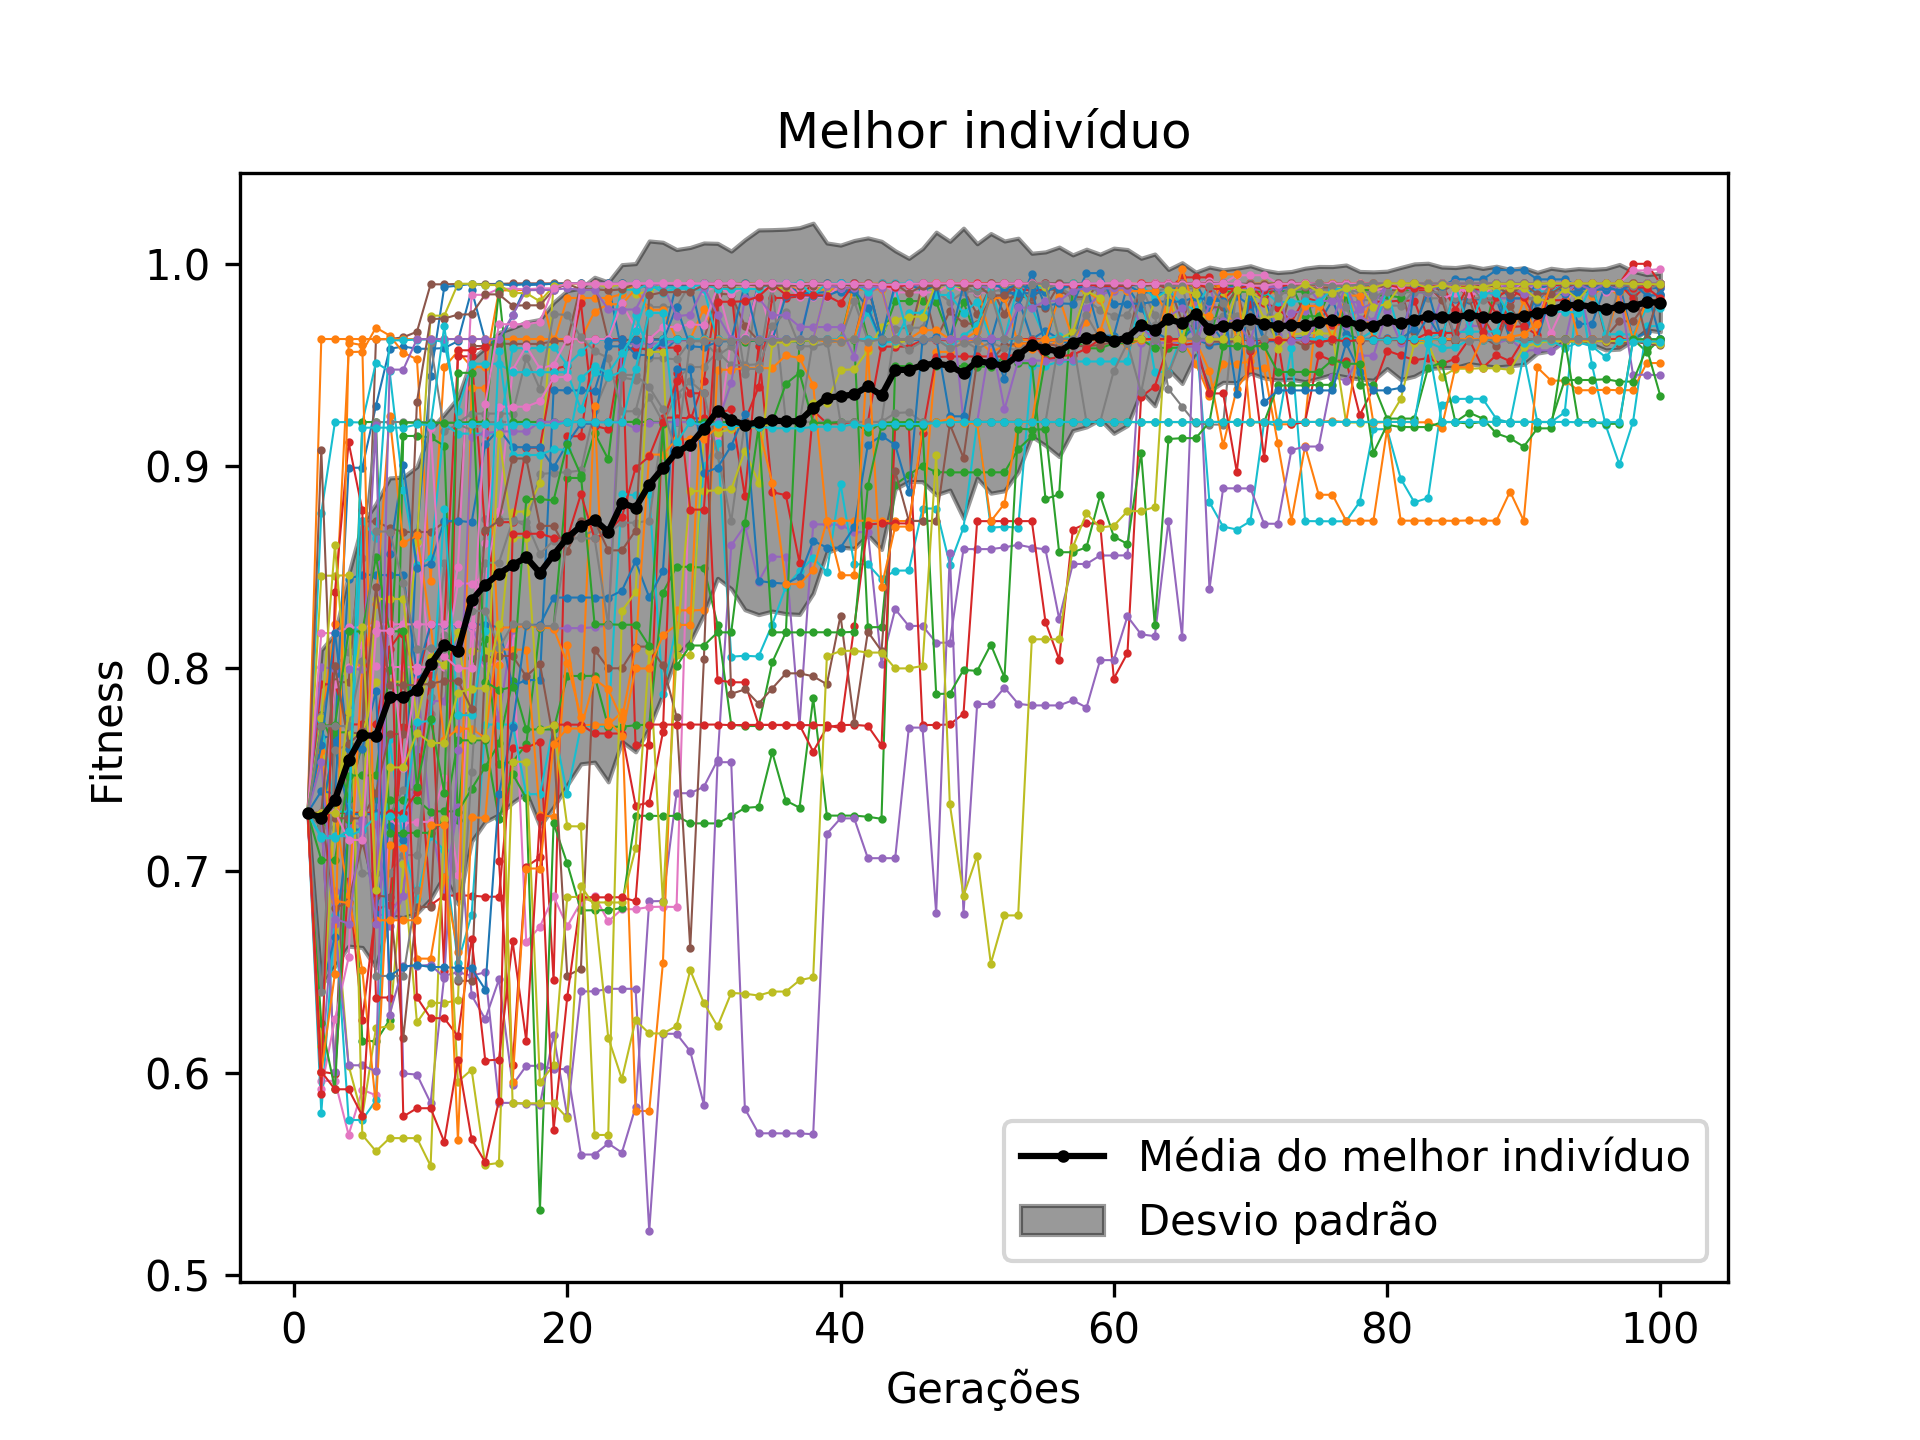
\includegraphics[width=1\textwidth]{sec-02/f6_10p_fitness_vs_gen_best.png}
		\caption{Melhores indíviduos de todos os experimentos ao longo das gerações.
		Em preto é mostrado o comportamento médio dos 50 experimentos. }
	\end{subfigure}
	\hfill
	\begin{subfigure}{.45\textwidth}
		\centering
		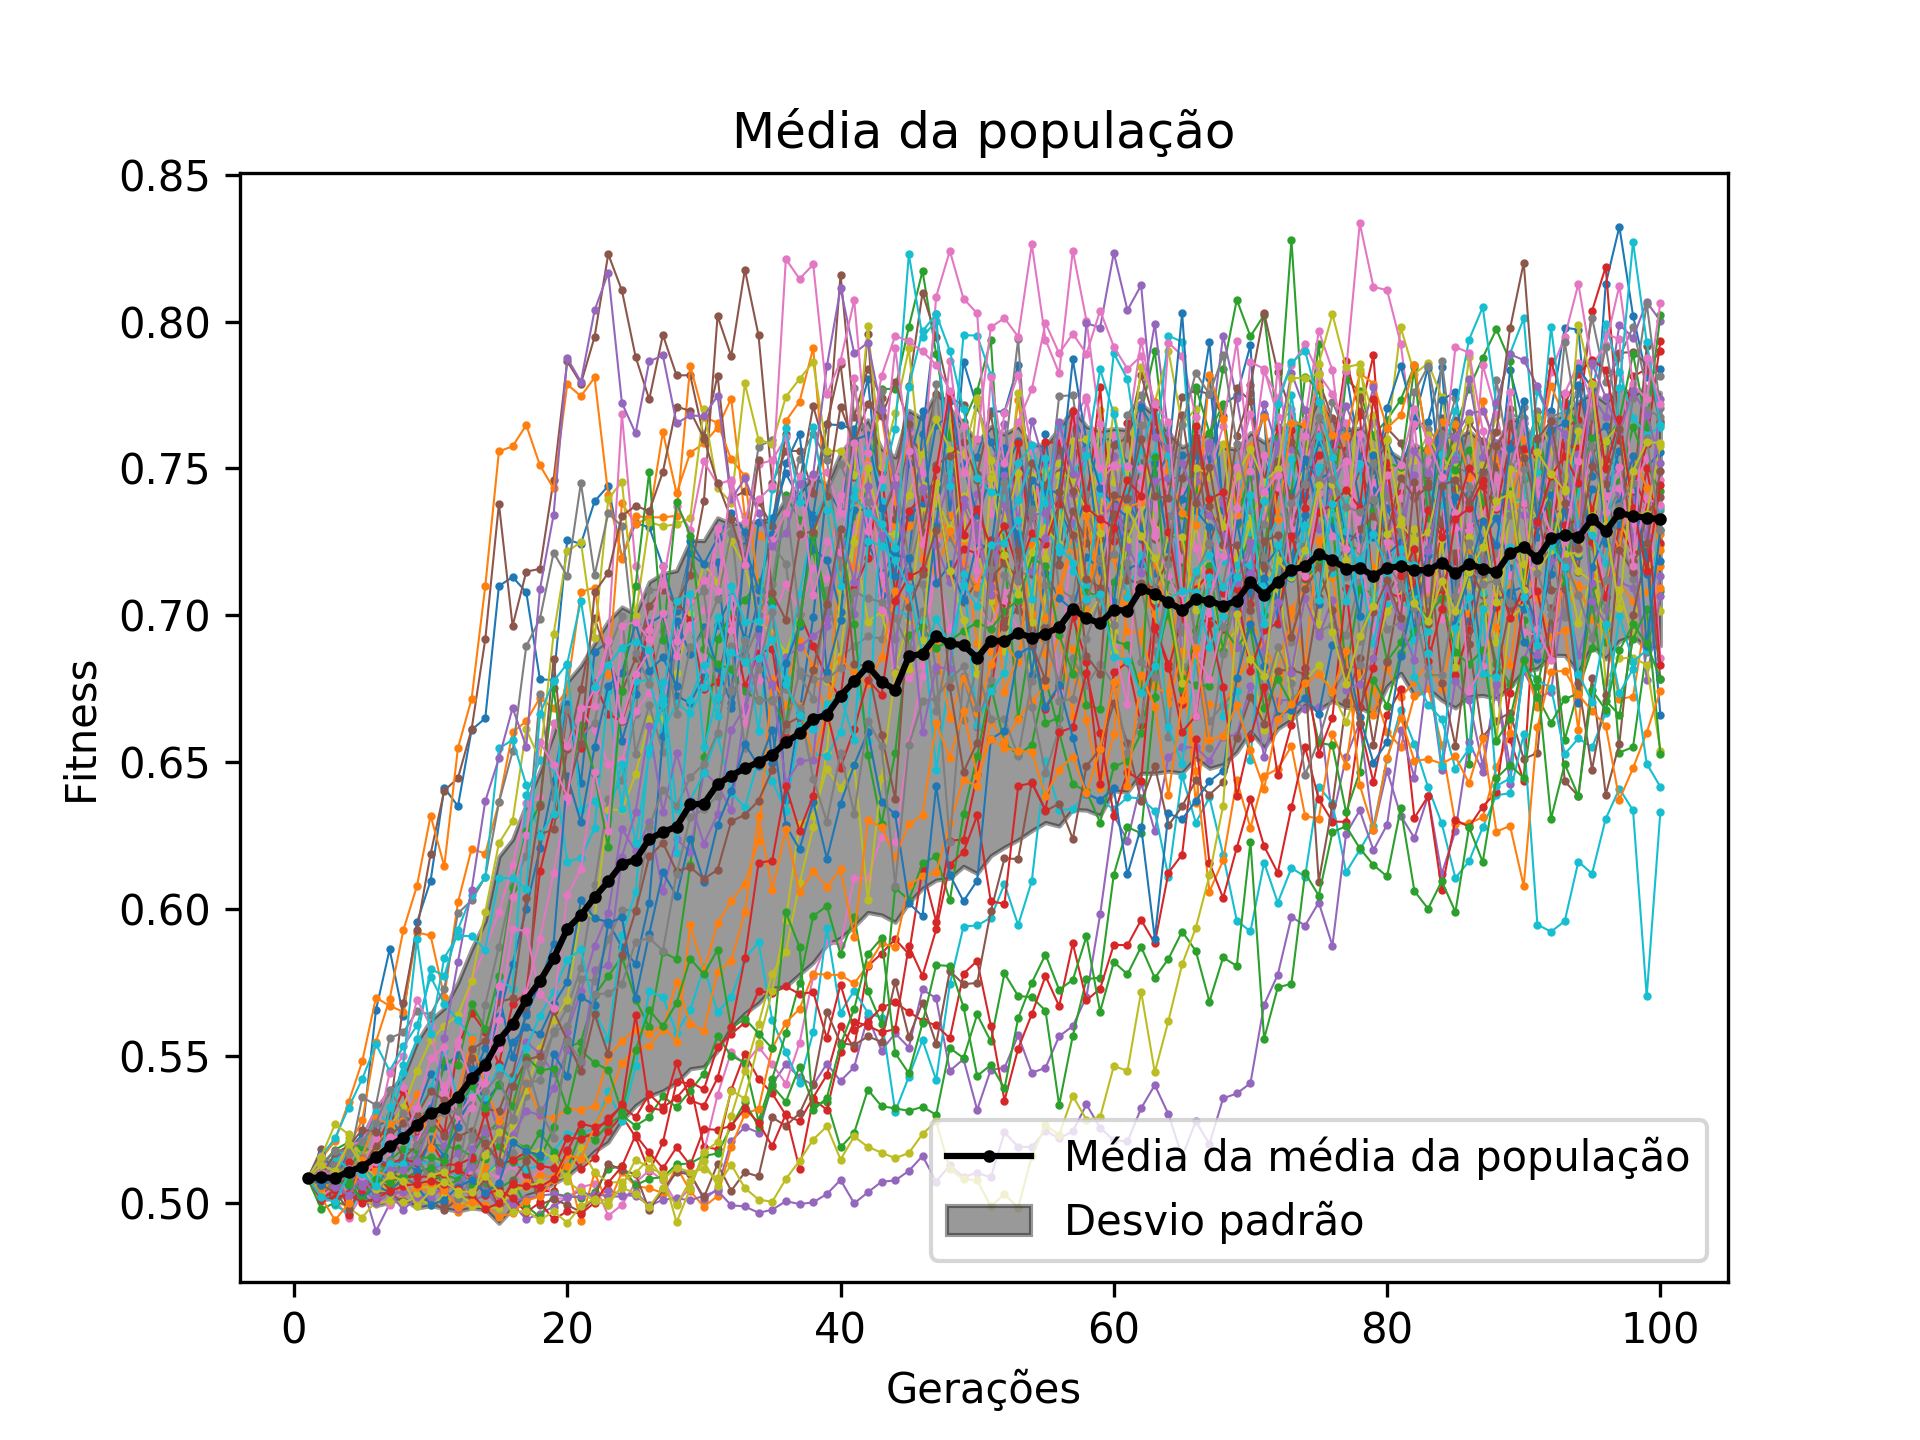
\includegraphics[width=1\textwidth]{sec-02/f6_10p_fitness_vs_gen_pop.png}
		\caption{Média da população de todos os experimentos ao longo das gerações.
		Em preto é mostrado o comportamento médio dos 50 experimentos.}
	\end{subfigure}
	\caption{Resultados obtidos para o caso de cruzamento de 10 pontos apresentado na tabela~\ref{tab:f6_crux}}
\end{figure}


	\begin{figure}[htb]
	\begin{subfigure}{.45\textwidth}
		\centering
		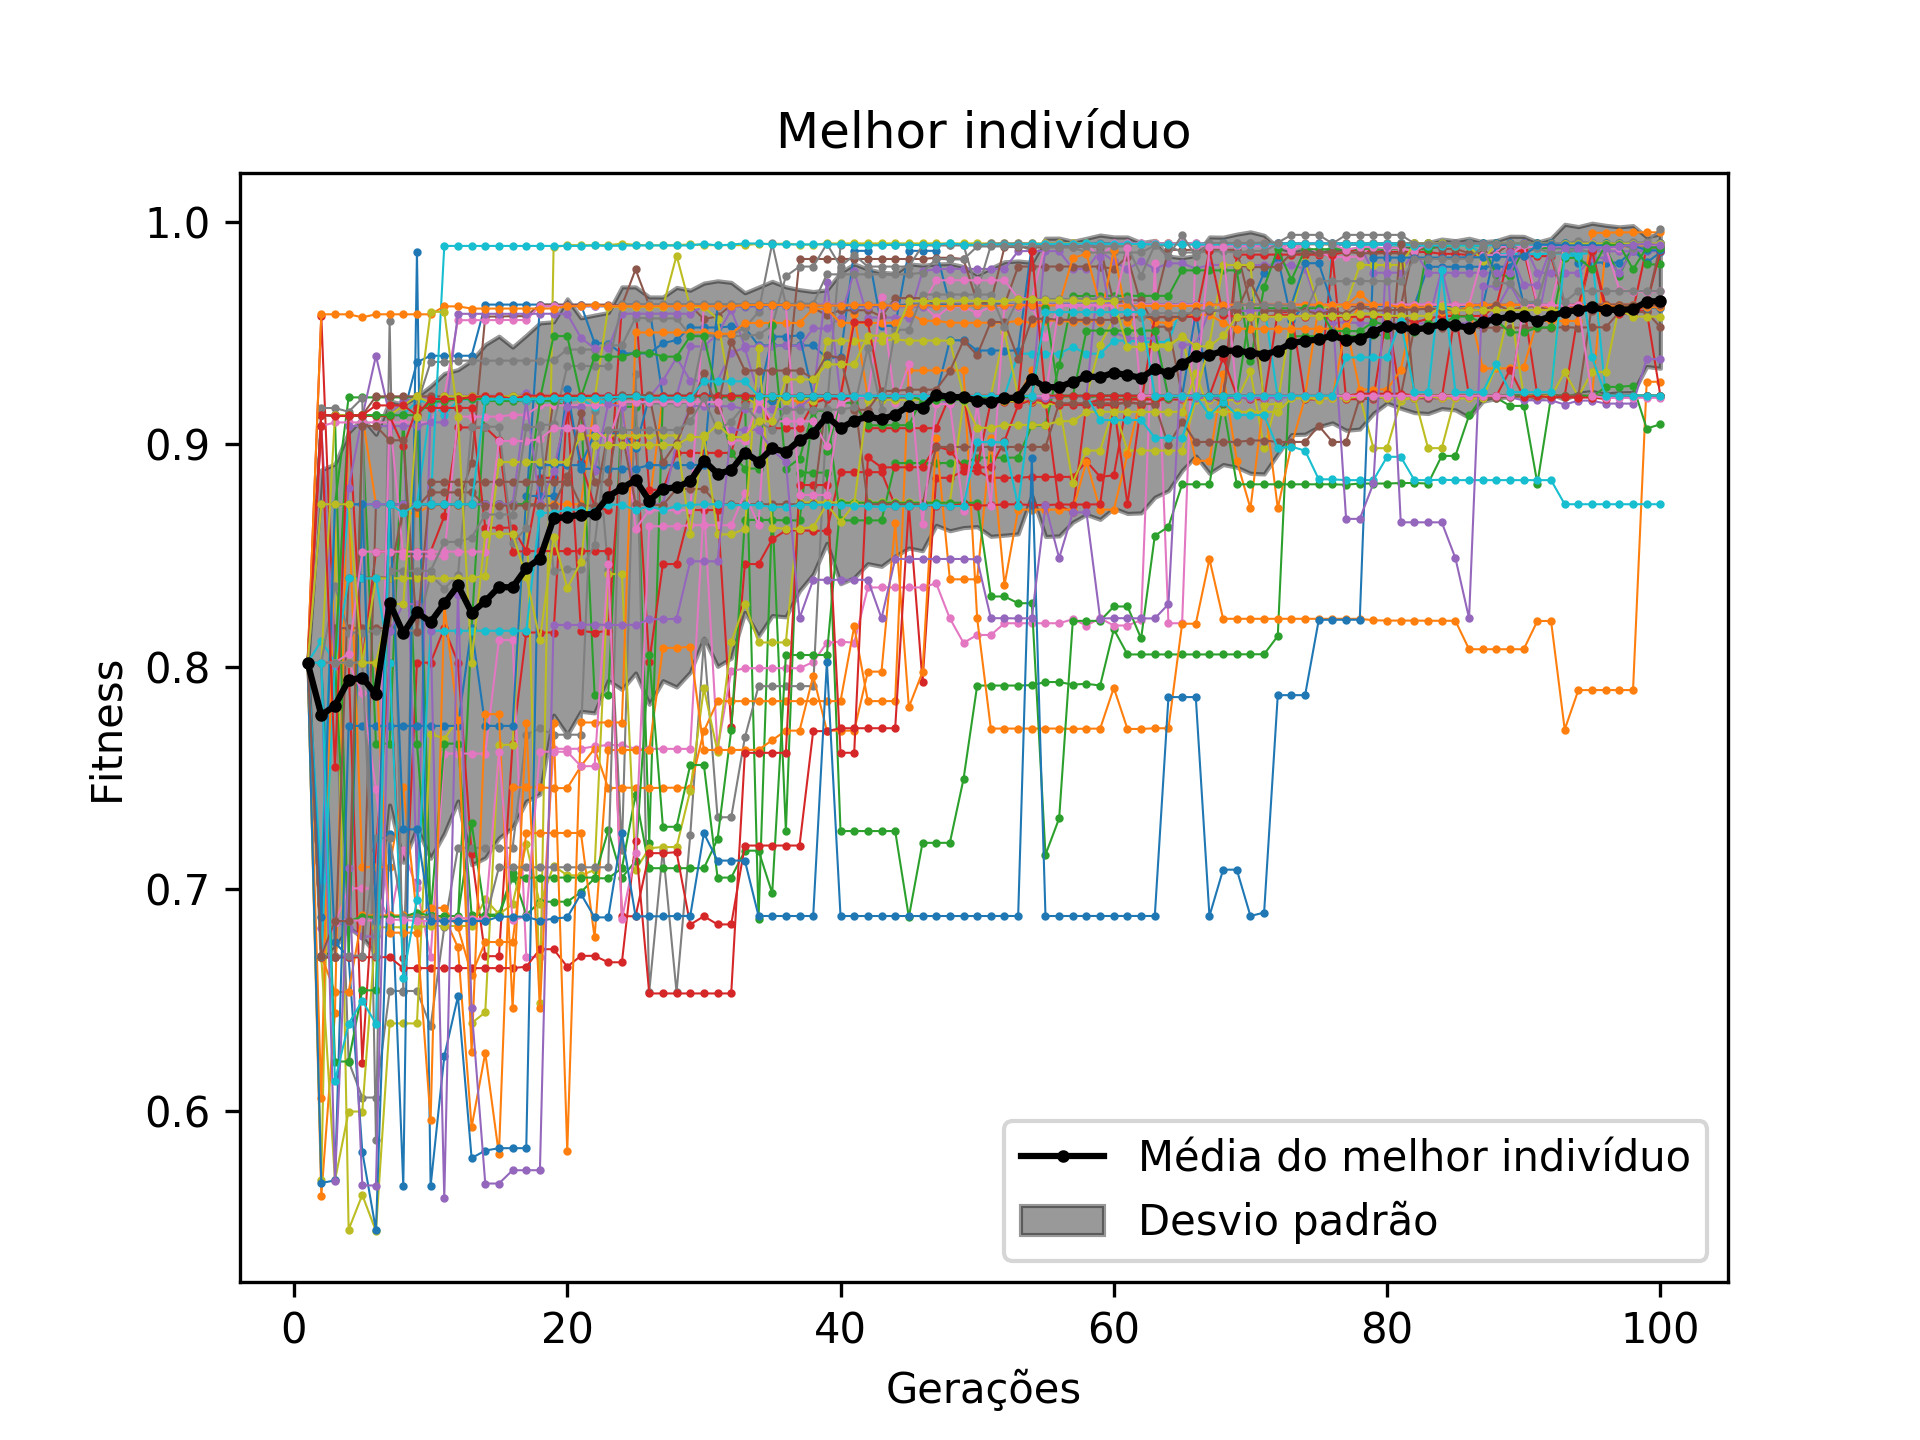
\includegraphics[width=1\textwidth]{sec-02/f6_u_fitness_vs_gen_best.png}
		\caption{Melhores indíviduos de todos os experimentos ao longo das gerações.
		Em preto é mostrado o comportamento médio dos 50 experimentos. }
	\end{subfigure}
	\hfill
	\begin{subfigure}{.45\textwidth}
		\centering
		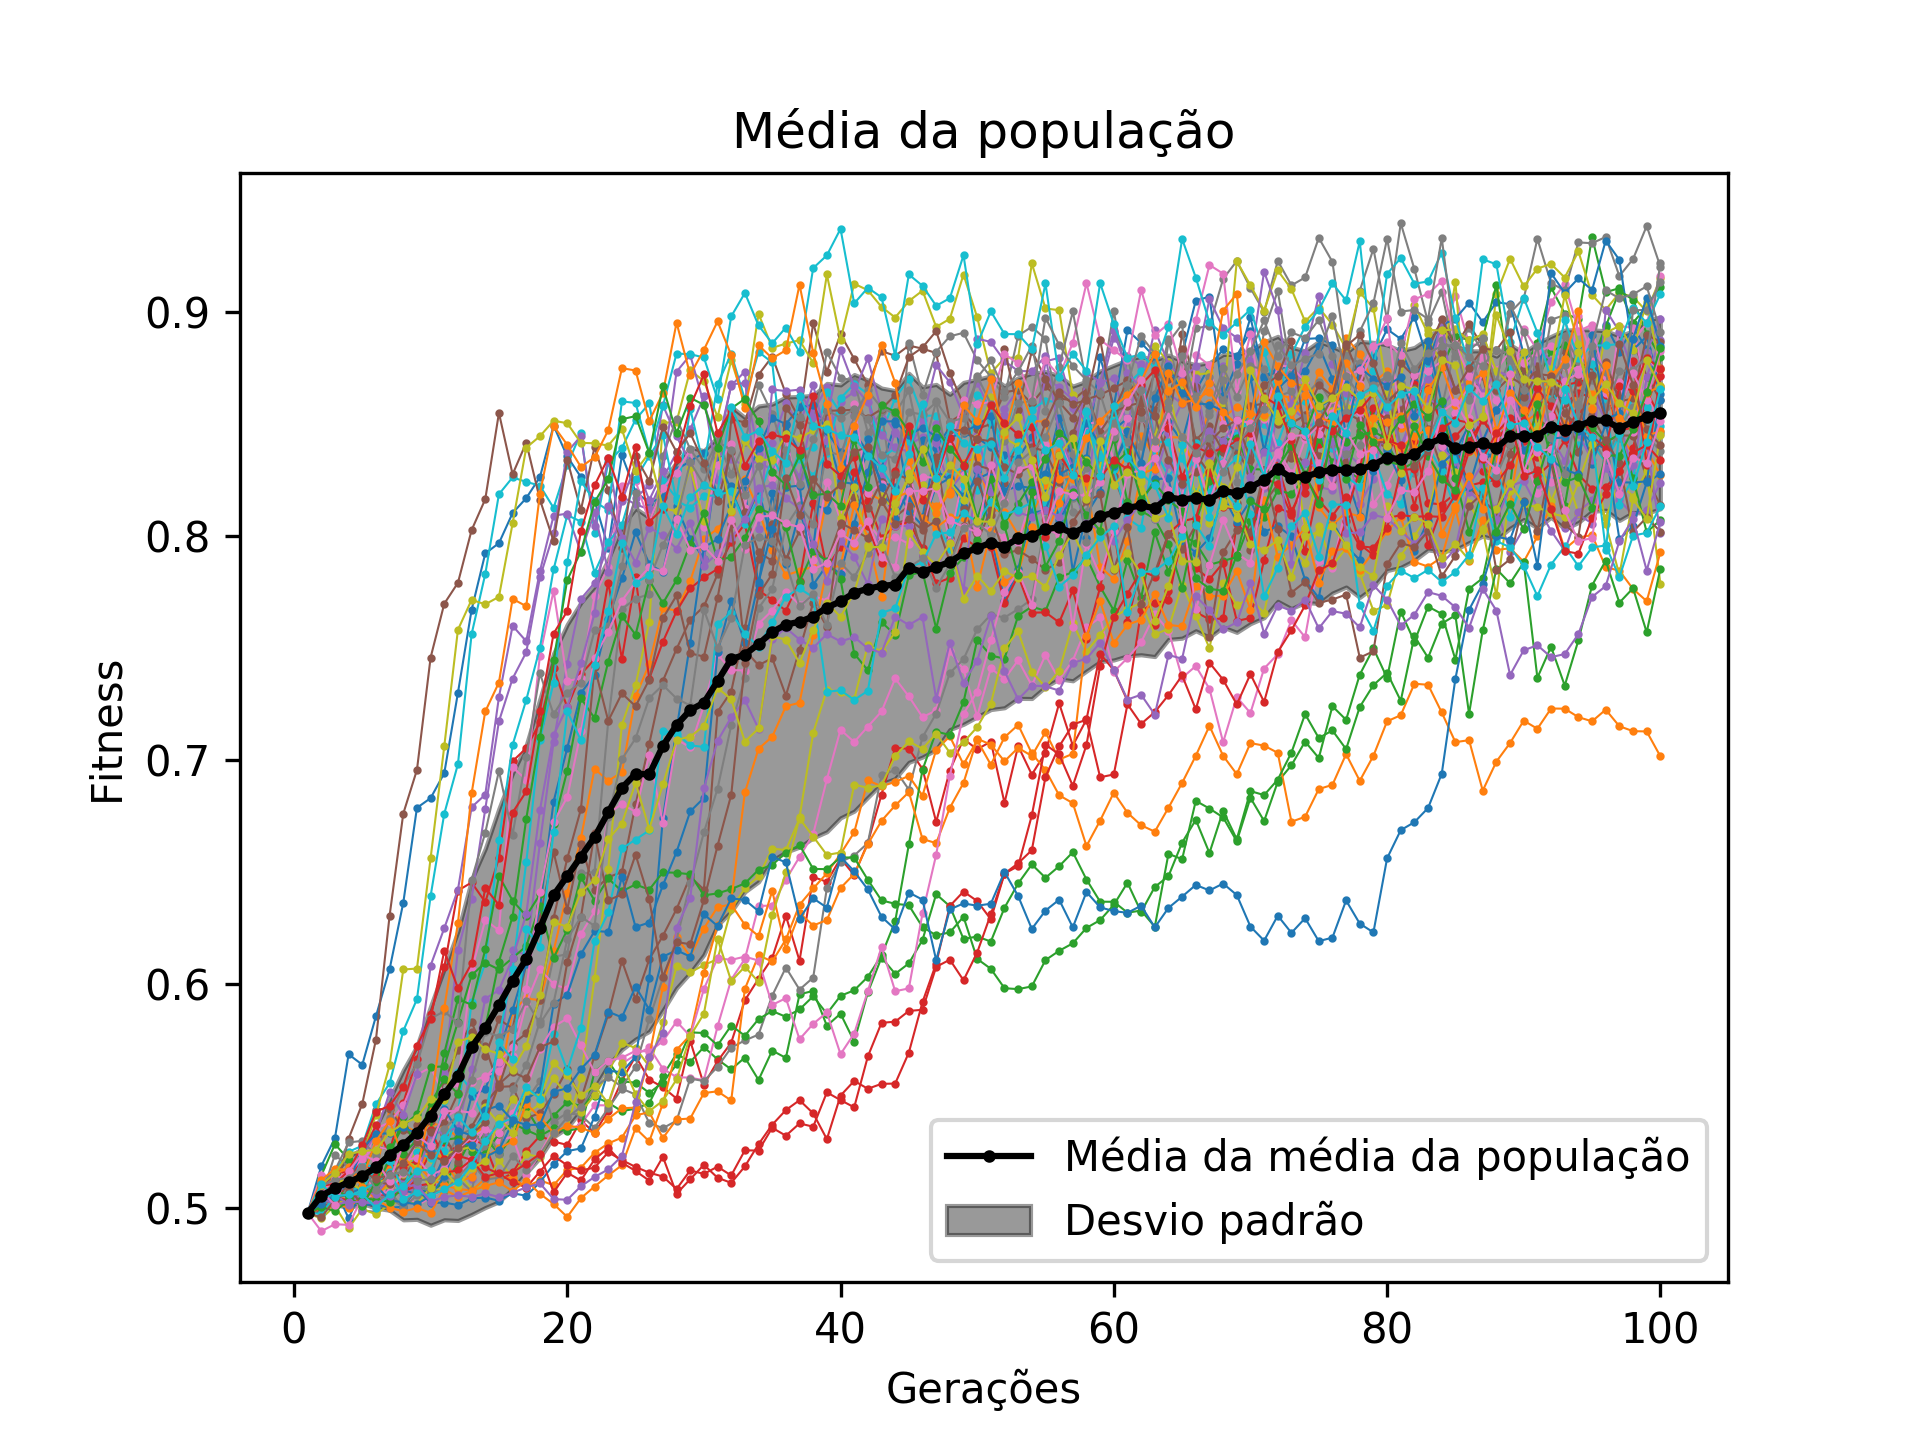
\includegraphics[width=1\textwidth]{sec-02/f6_u_fitness_vs_gen_pop.png}
		\caption{Média da população de todos os experimentos ao longo das gerações.
		Em preto é mostrado o comportamento médio dos 50 experimentos.}
	\end{subfigure}
	\caption{Resultados obtidos para o caso de cruzamento uniforme apresentado na tabela~\ref{tab:f6_crux}}
\end{figure}

	\clearpage
	\section{Representação real}
		Para problemas como o de otimização de funções, onde o dominio do problema é real, a
representação do cromossomo também pode ser real. Nesse caso, a representação irá
trabalhar diretamente no espaço de busca, sem a necessidade de codificar e decodificar
como no caso binário.

Portanto para representar o problema da otimização da função $f6$, a seguinte configuração foi utilizada:
\begin{itemize}
	\item Representação: Representação real dentro do intervalo $[-100,100]$. Assim, o cromossomo é composto por um vetor de duas posições.

	\item Seleção: Foi utilizados a roleta proporcional ao fitness tanto para a função $f6$
		quanto para a função $f6_{elevada}$.

    \item Operadores genéticos: Para realizar o cruzamento, foi utilizado o algoritmo
    aritmético com uma taxa de cruzamento de 75\%. Também, foi utilizada mutação uniforme
    com uma taxa igual a 1\%.
	\item Critério de paragem: O critério de paragem foi 100 gerações.
\end{itemize}

Assim, foram obtidos os resultados apresentados na tabela \ref{tab:f6_real}.

\begin{table}[htb]
	\centering
	\begin{tabular}{|c|c|c|}
		\hline
		\rowcolor[HTML]{9B9B9B}
		Teste & Média melhor indíviduo & Média população \\\hline
		1 & 0.94825 & 0.89753 \\\hline
		2 & 0.96592 & 0.91702 \\\hline
		3 & 0.95119 & 0.89079 \\\hline
		4 & 0.95656 & 0.90589 \\\hline
		5 & 0.95067 & 0.89339 \\\hline
		\textbf{Média Final} & \textbf{0.954518} & \textbf{0.90092} \\\hline	\end{tabular}
	\caption{Resultados da função $f6$ utilizando representação real, cruzamento aritmético e mutação uniforme \label{tab:f6_real}}
\end{table}

Adicionando elitismo no AG acima, temos um aumento de performance significativo, como mostrado
na tabela~\ref{tab:f6_real_elite}

\begin{table}[htb]
	\centering
	\begin{tabular}{|c|c|c|}
		\hline
		\rowcolor[HTML]{9B9B9B}
		Teste & Média melhor indíviduo & Média população \\\hline
		1 & 0.98896 & 0.94950 \\\hline
		2 & 0.98978 & 0.93423 \\\hline
		3 & 0.98952 & 0.94188 \\\hline
		4 & 0.98867 & 0.94448 \\\hline
		5 & 0.98964 & 0.92809 \\\hline
		\textbf{Média Final} & \textbf{0.98932} & \textbf{0.93963} \\\hline	\end{tabular}
    \caption{Resultados da função $f6$ utilizando representação real, cruzamento aritmético,
    mutação uniforme e elitismo. \label{tab:f6_real_elite}}
\end{table}

\begin{figure}[htb]
	\begin{subfigure}{.45\textwidth}
		\centering
		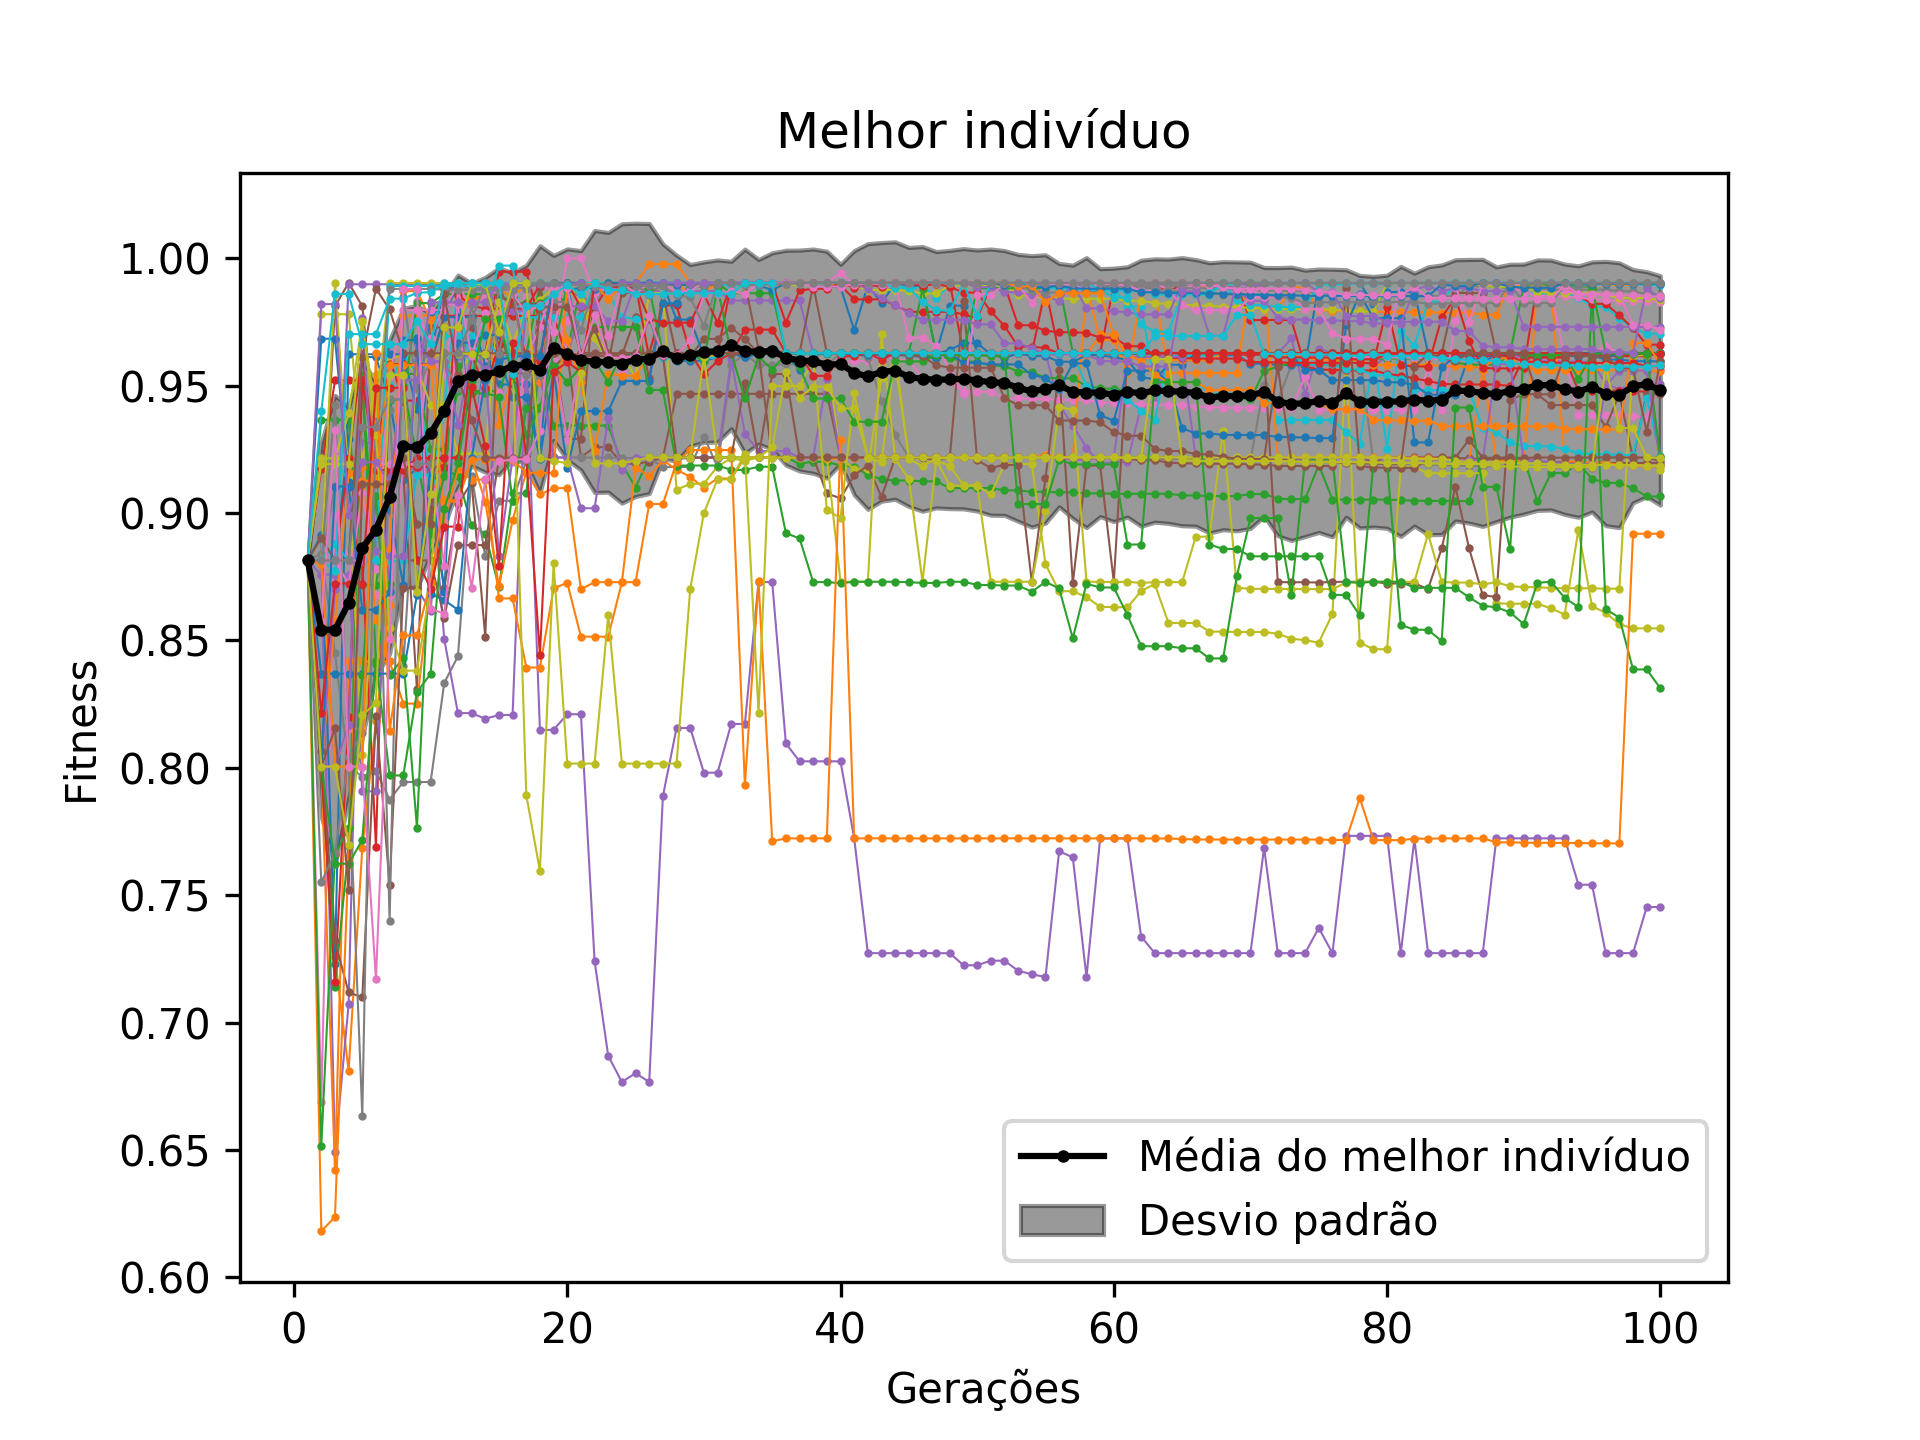
\includegraphics[width=1\textwidth]{sec-03/f6_real_fitness_vs_gen_best.png}
		\caption{Melhores indíviduos de todos os experimentos ao longo das gerações.
		Em preto é mostrado o comportamento médio dos 50 experimentos. }
	\end{subfigure}
	\hfill
	\begin{subfigure}{.45\textwidth}
		\centering
		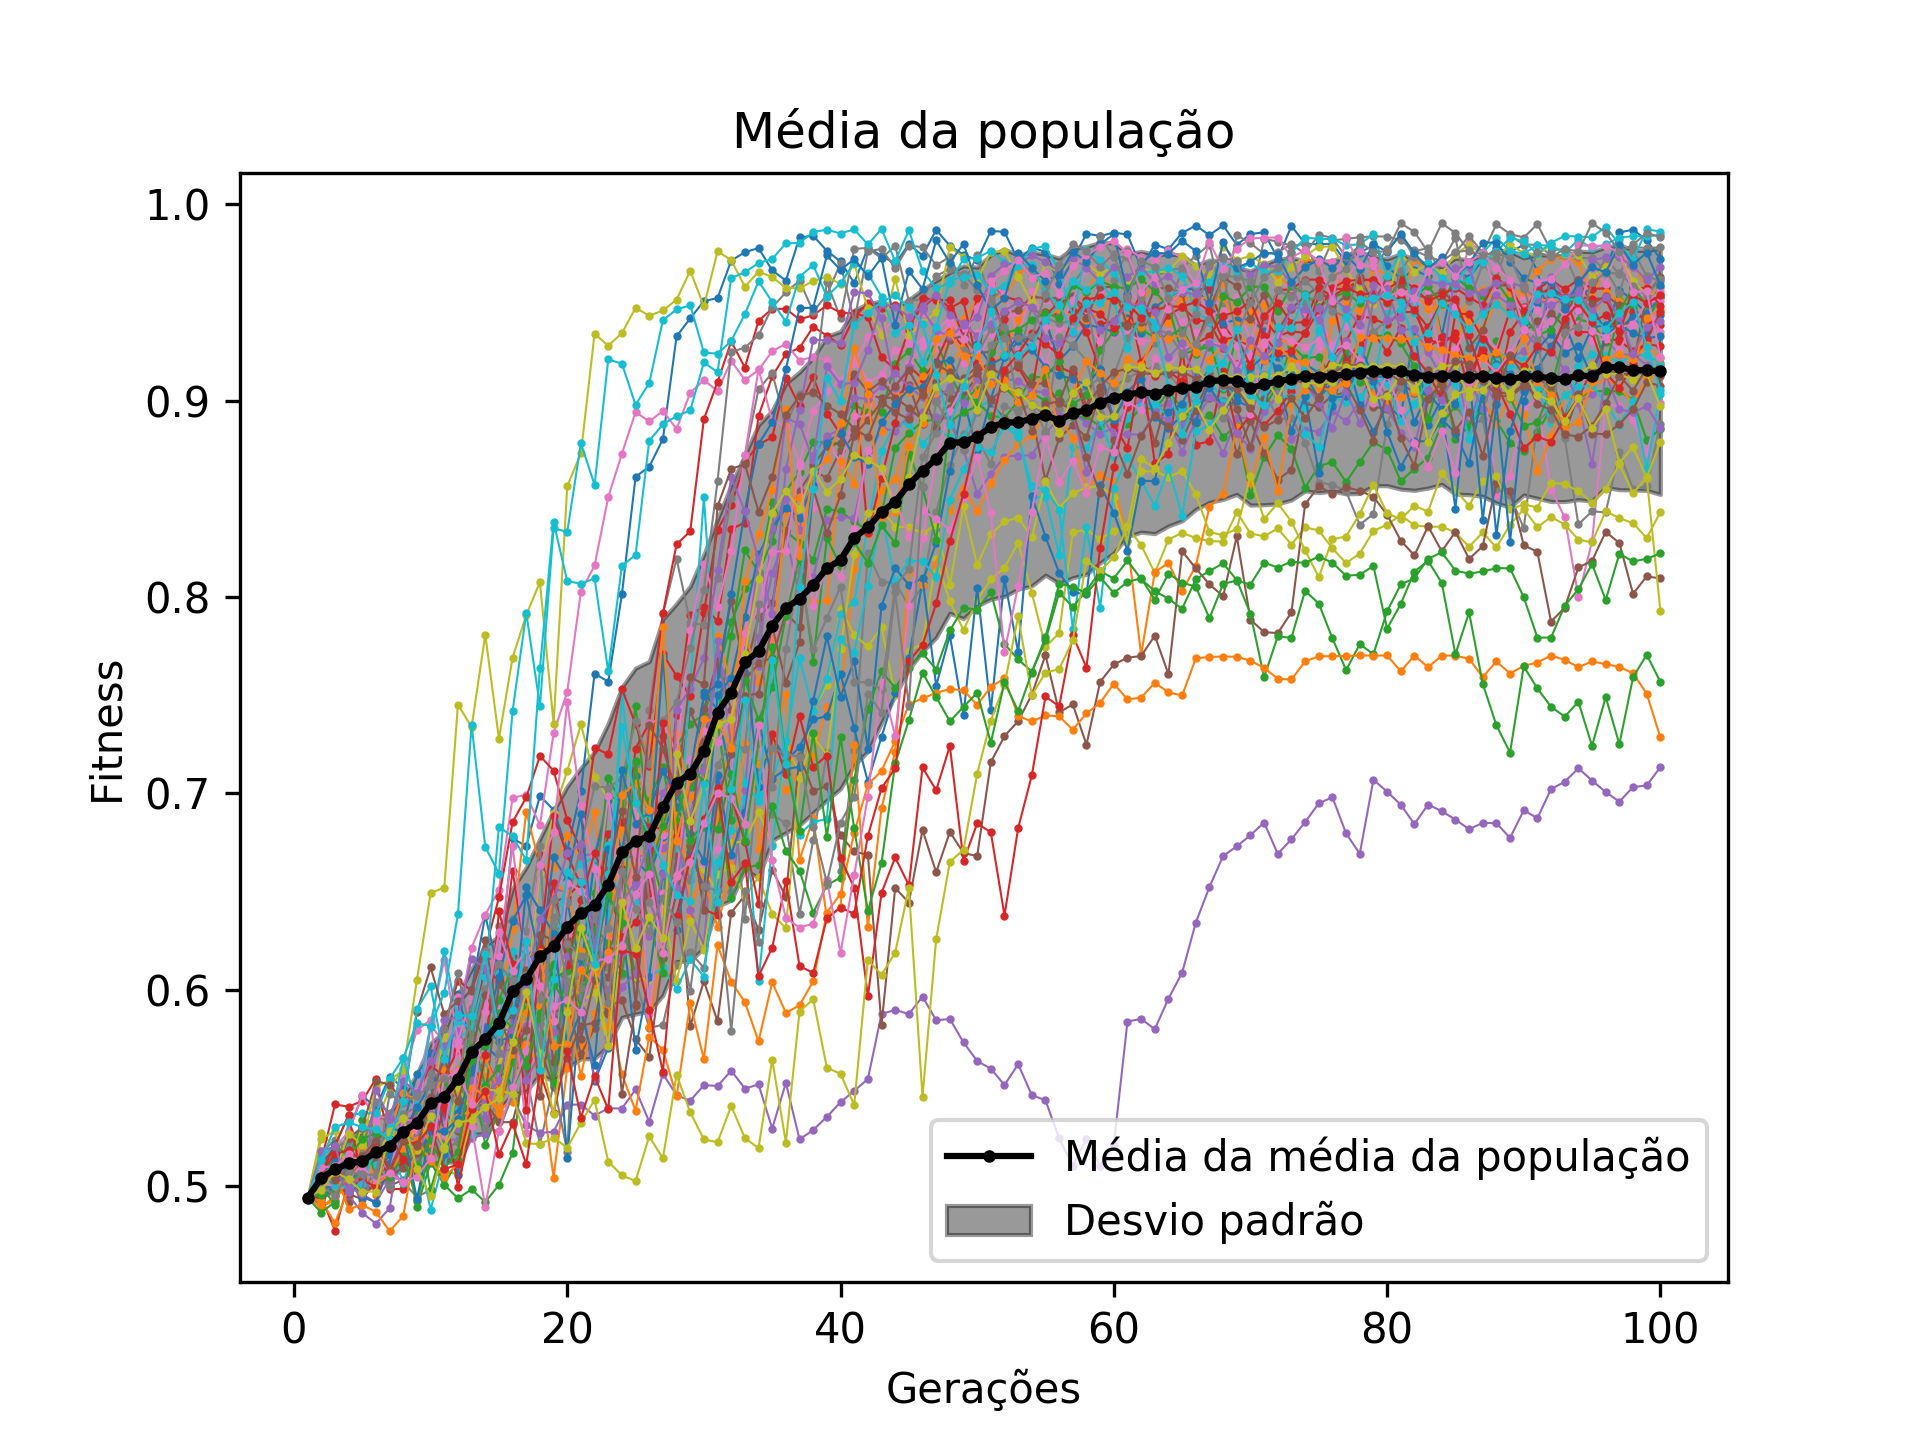
\includegraphics[width=1\textwidth]{sec-03/f6_real_fitness_vs_gen_pop.png}
		\caption{Média da população de todos os experimentos ao longo das gerações.
		Em preto é mostrado o comportamento médio dos 50 experimentos.}
	\end{subfigure}
	\caption{Resultados obtidos utilizando utilizando representação real, cruzamento aritmético e
    mutação uniforme}
\end{figure}


	\begin{figure}[htb]
	\begin{subfigure}{.45\textwidth}
		\centering
		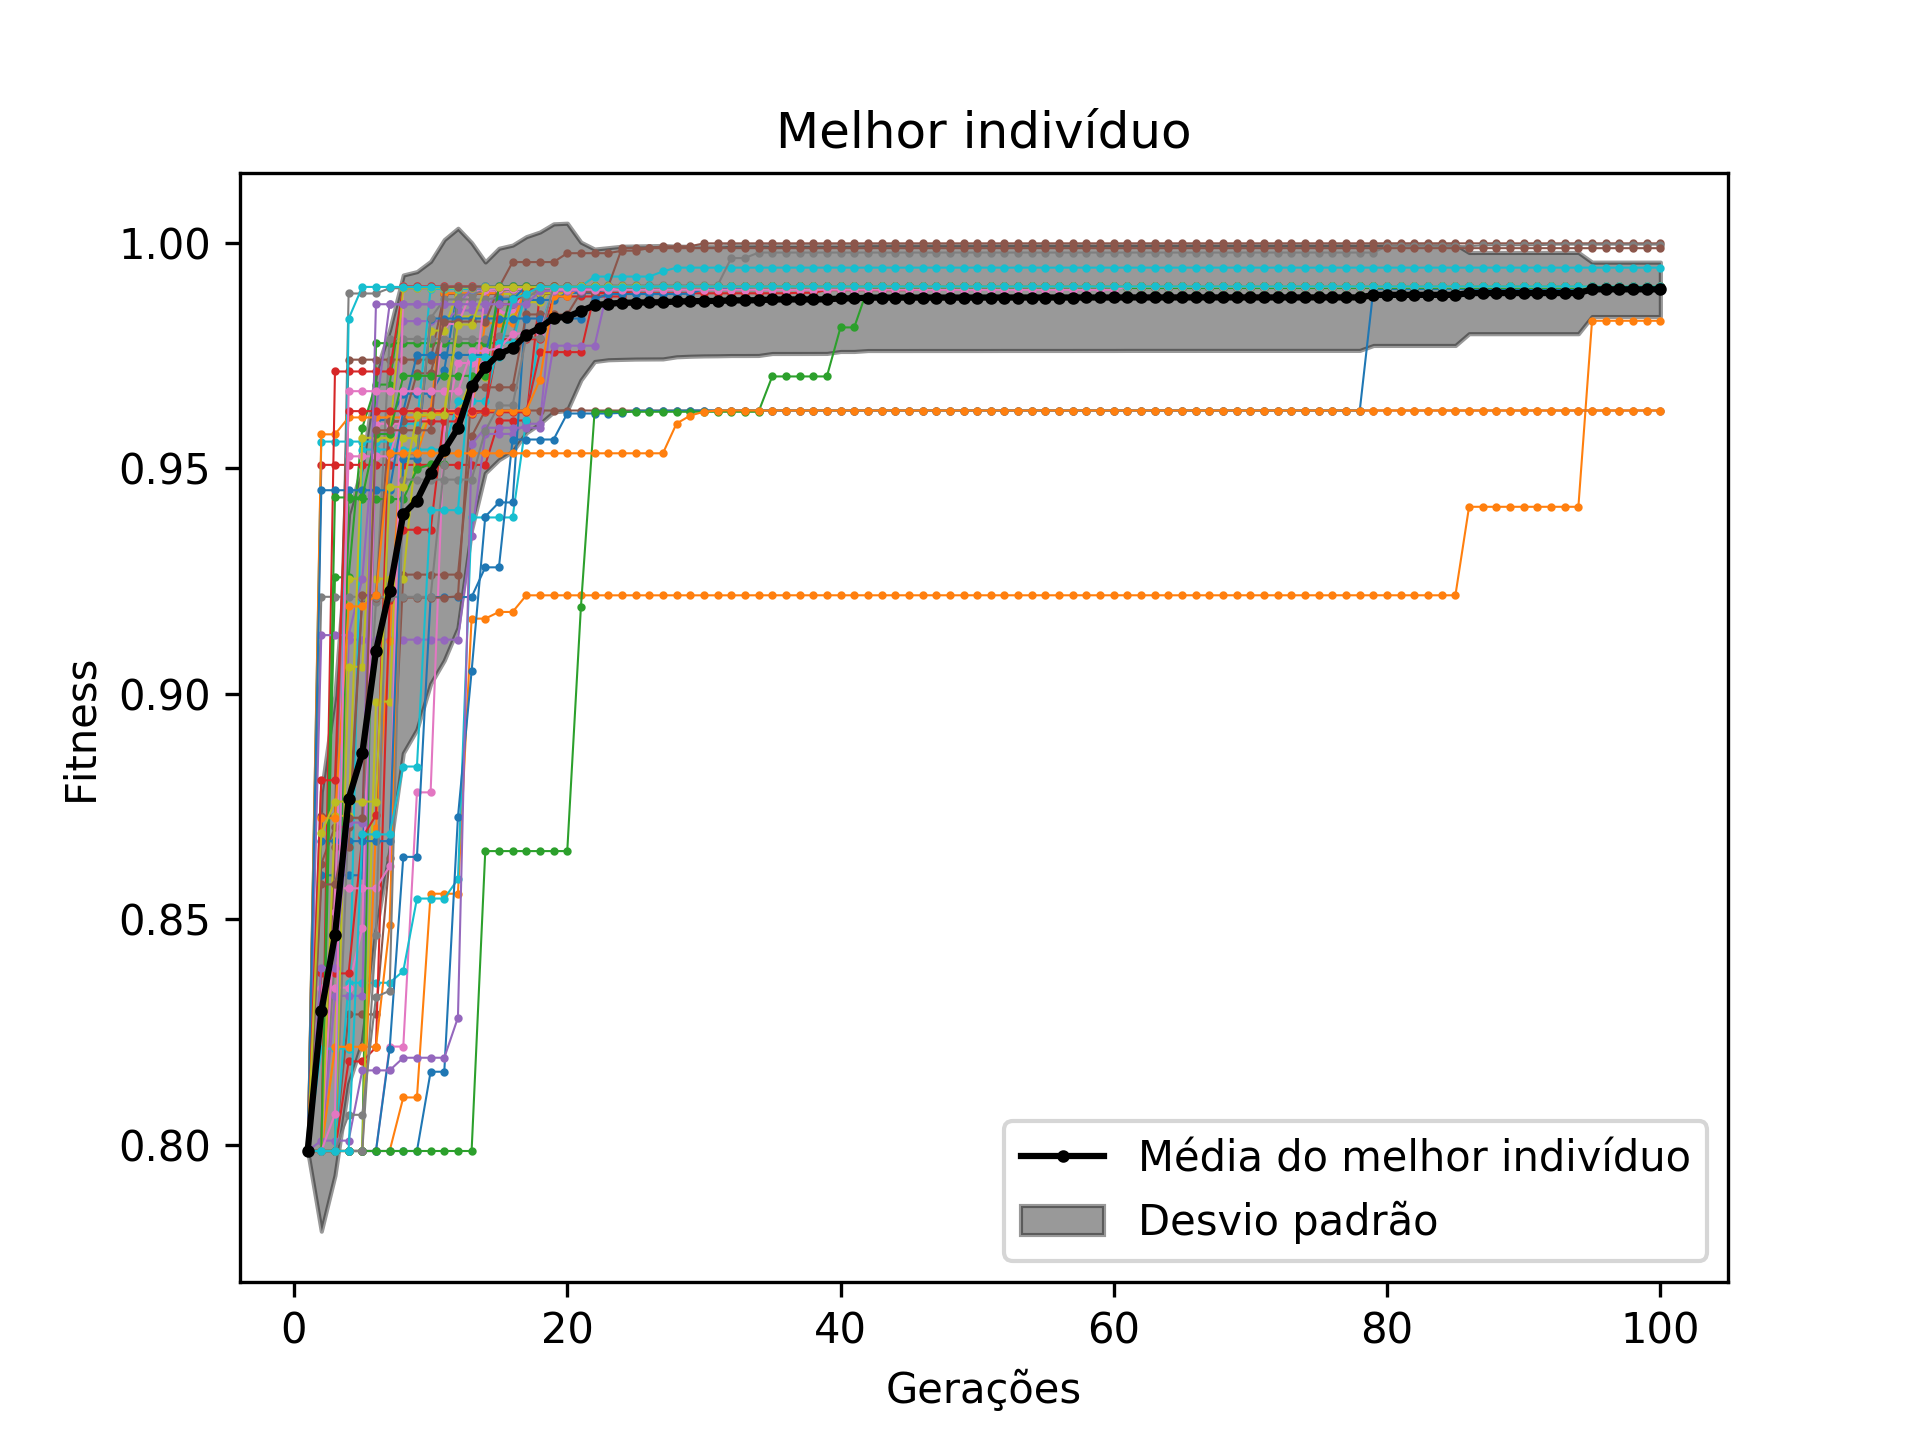
\includegraphics[width=1\textwidth]{sec-03/f6_real_elite_fitness_vs_gen_best.png}
		\caption{Melhores indíviduos de todos os experimentos ao longo das gerações.
		Em preto é mostrado o comportamento médio dos 50 experimentos. }
	\end{subfigure}
	\hfill
	\begin{subfigure}{.45\textwidth}
		\centering
		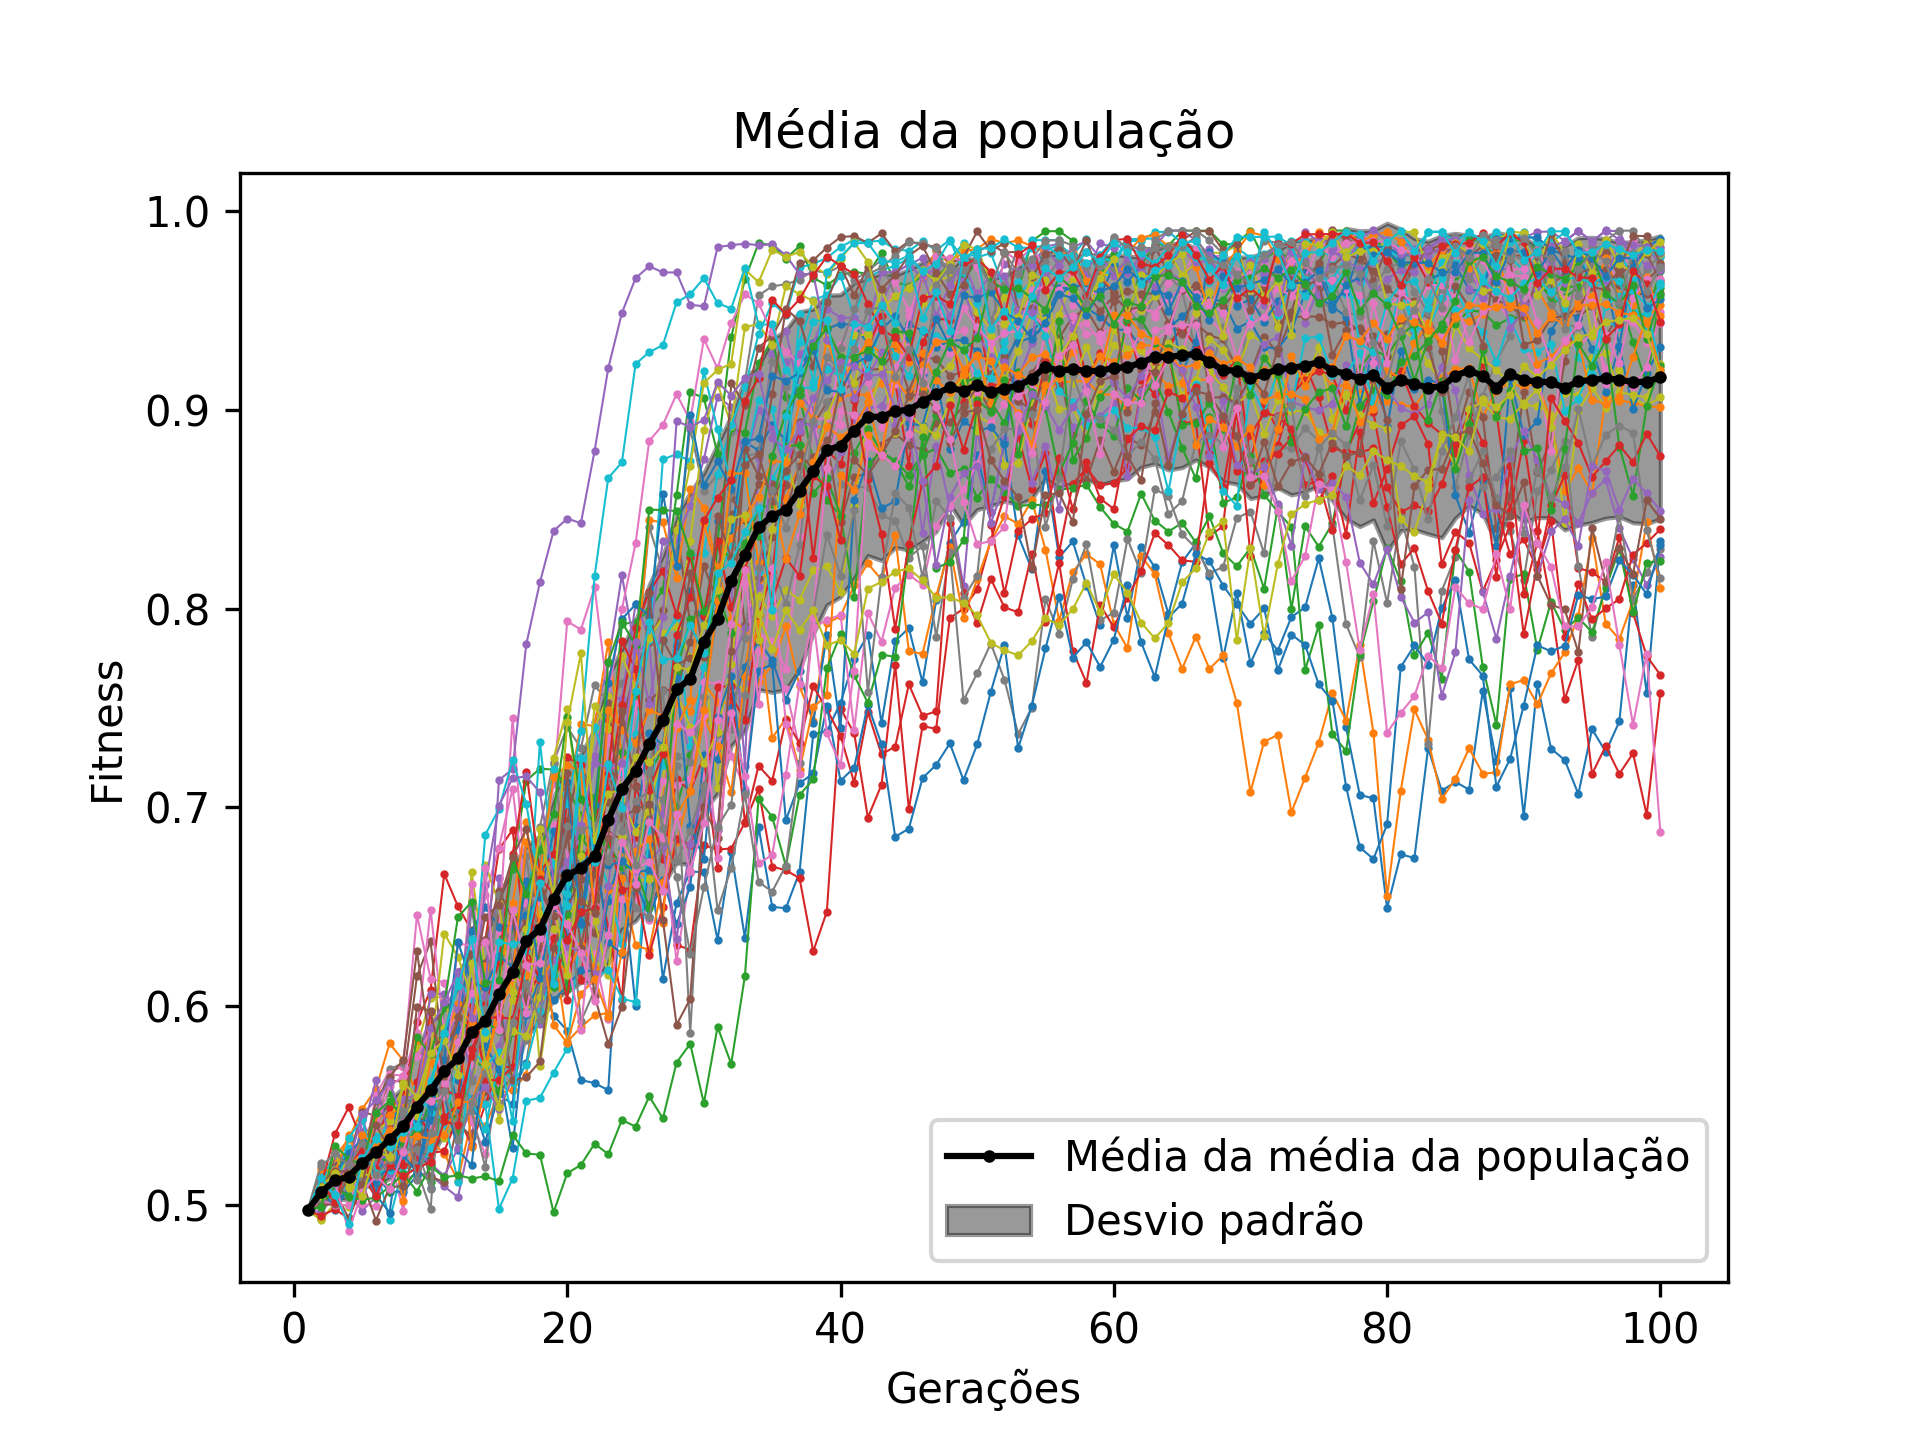
\includegraphics[width=1\textwidth]{sec-03/f6_real_elite_fitness_vs_gen_pop.png}
		\caption{Média da população de todos os experimentos ao longo das gerações.
		Em preto é mostrado o comportamento médio dos 50 experimentos.}
	\end{subfigure}
	\caption{Resultados obtidos utilizando representação real, cruzamento aritmético,
    mutação uniforme e elitismo}
\end{figure}

	\clearpage
	\section{Função F6 com 10 variáveis}
		Para o caso de uma função F6 com 10 variáveis, temos que:

\begin{equation}
    \begin{split}
        F(x_1 .. x_{10}) = & F6(x_1, x_2) + F6(x_2, x_3) + F6(x_3, x_4) + F6(x_4, x_5) + F6(x_5, x_6) \\
                          & F6(x_6, x_7) + F6(x_7, x_8) + F6(x_8, x_9) + F6(x_9, x_{10})
    \end{split}
\end{equation}

Portanto a seguinte configuração foi utilizada:
\begin{itemize}
	\item Representação: Representação real com 10 variáveis dentro do intervalo $[-100,100]$. Assim, o cromossomo é composto por um vetor de 10 posições.

	\item Seleção: Foi utilizados a roleta proporcional ao fitness tanto para a função $f6$
        quanto para a função $f6_{elevada}$.

    \item O Método de elitismo foi utilizado.

    \item Operadores genéticos: Para realizar o cruzamento, foi utilizado o algoritmo
    aritmético com uma taxa de cruzamento de 75\%. Também, foi utilizada mutação uniforme
    com uma taxa igual a 1\%.

	\item Critério de paragem: O critério de paragem foi 100 gerações.
\end{itemize}

Os resultados obtidos são apresentados na tabela~\ref{tab:f6_10}.

\begin{table}[htb]
	\centering
	\begin{tabular}{|c|c|c|}
		\hline
		\rowcolor[HTML]{9B9B9B}
		Teste & Média melhor indíviduo & Média população \\\hline
		1 & 7.23983 & 5.33647 \\\hline
		2 & 7.27323 & 5.29675 \\\hline
		3 & 7.32053 & 5.36799 \\\hline
		4 & 7.21803 & 5.31238 \\\hline
		5 & 7.31284 & 5.36265 \\\hline
		\textbf{Média Final} & \textbf{7.27289} & \textbf{5.33523} \\\hline	\end{tabular}
    \caption{Resultados da função $f6$ utilizando representação real, cruzamento aritmético,
    mutação uniforme e elitismo. \label{tab:f6_10}}
\end{table}

\begin{figure}[htb]
	\begin{subfigure}{.45\textwidth}
		\centering
		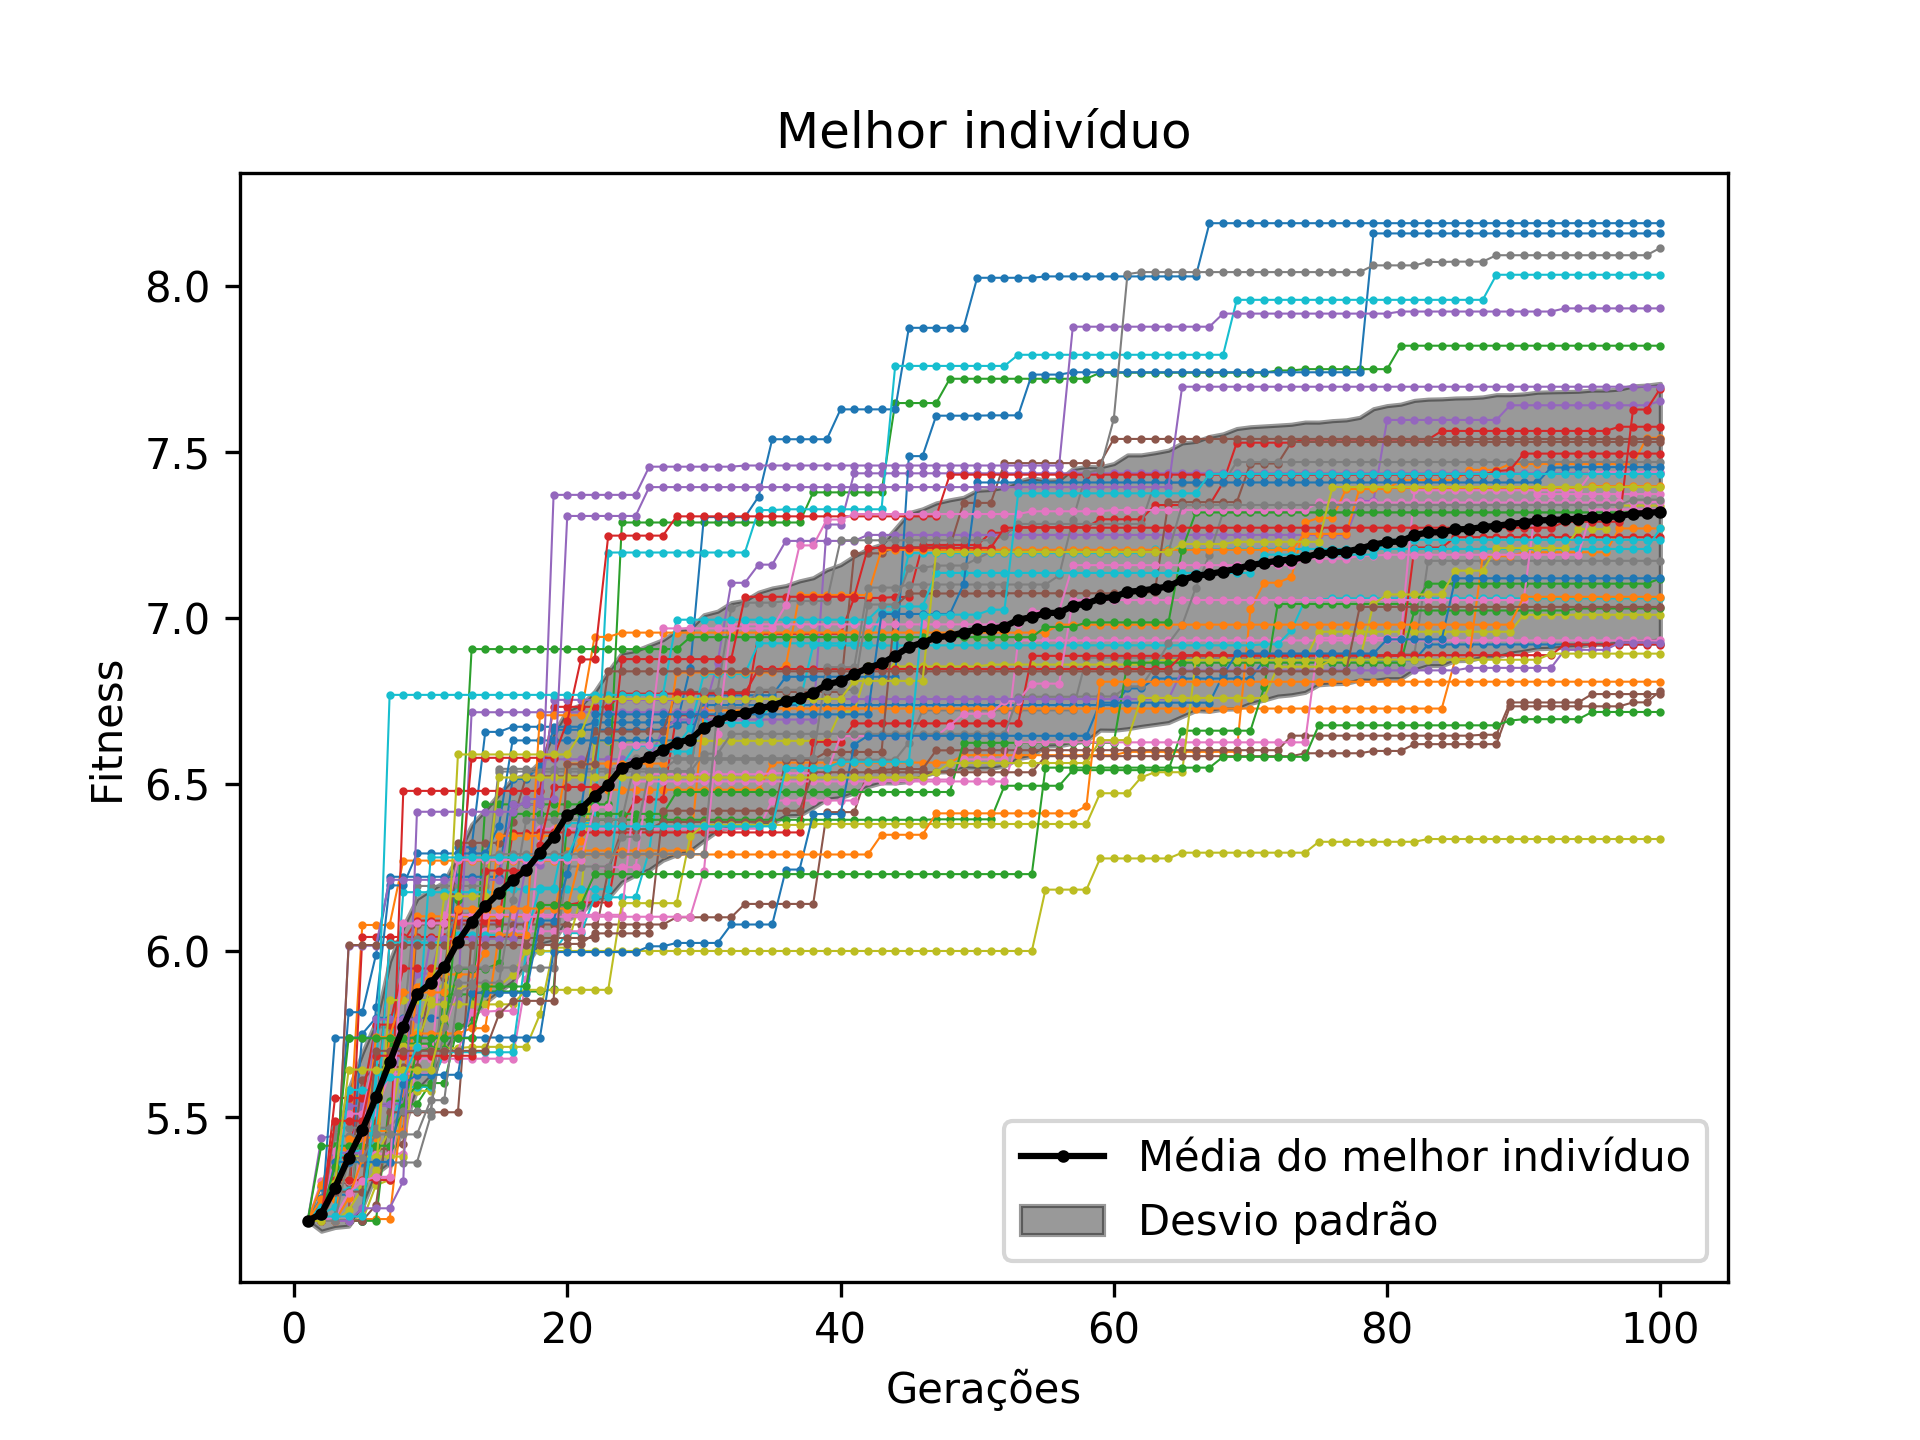
\includegraphics[width=1\textwidth]{sec-04/f6_fitness_vs_gen_best.png}
		\caption{Melhores indíviduos de todos os experimentos ao longo das gerações.
		Em preto é mostrado o comportamento médio dos 50 experimentos. }
	\end{subfigure}
	\hfill
	\begin{subfigure}{.45\textwidth}
		\centering
		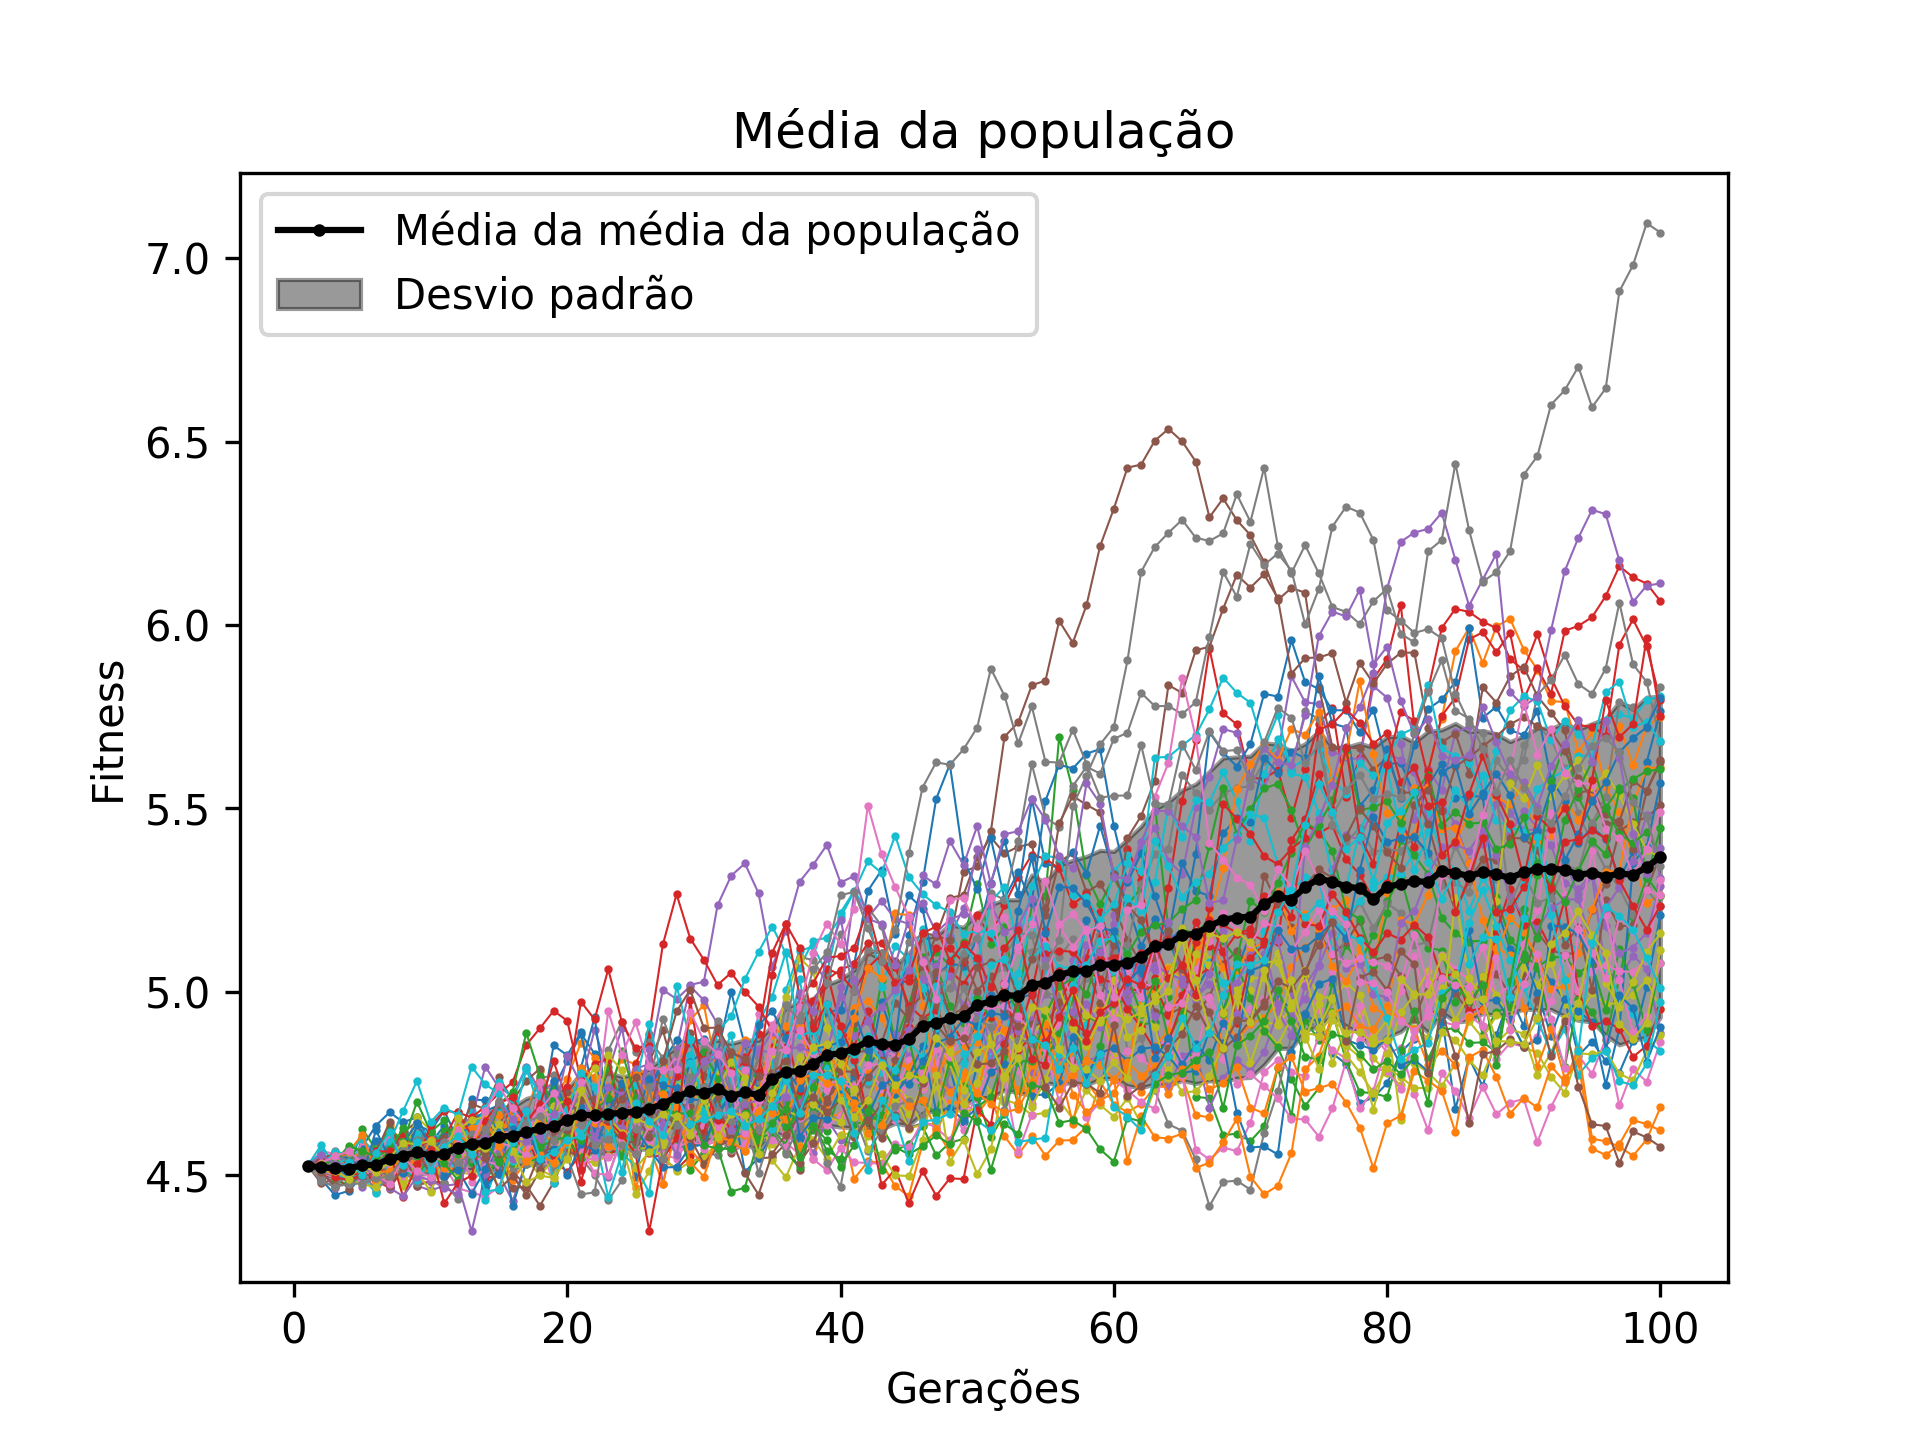
\includegraphics[width=1\textwidth]{sec-04/f6_fitness_vs_gen_pop.png}
		\caption{Média da população de todos os experimentos ao longo das gerações.
		Em preto é mostrado o comportamento médio dos 50 experimentos.}
	\end{subfigure}
	\caption{Resultados obtidos utilizando utilizando representação real, cruzamento aritmético,
    mutação uniforme e elitimo para o caso da F6 com 10 variáveis.}
\end{figure}

\begin{figure}[htb]
	\begin{subfigure}{.5\textwidth}
		\centering
		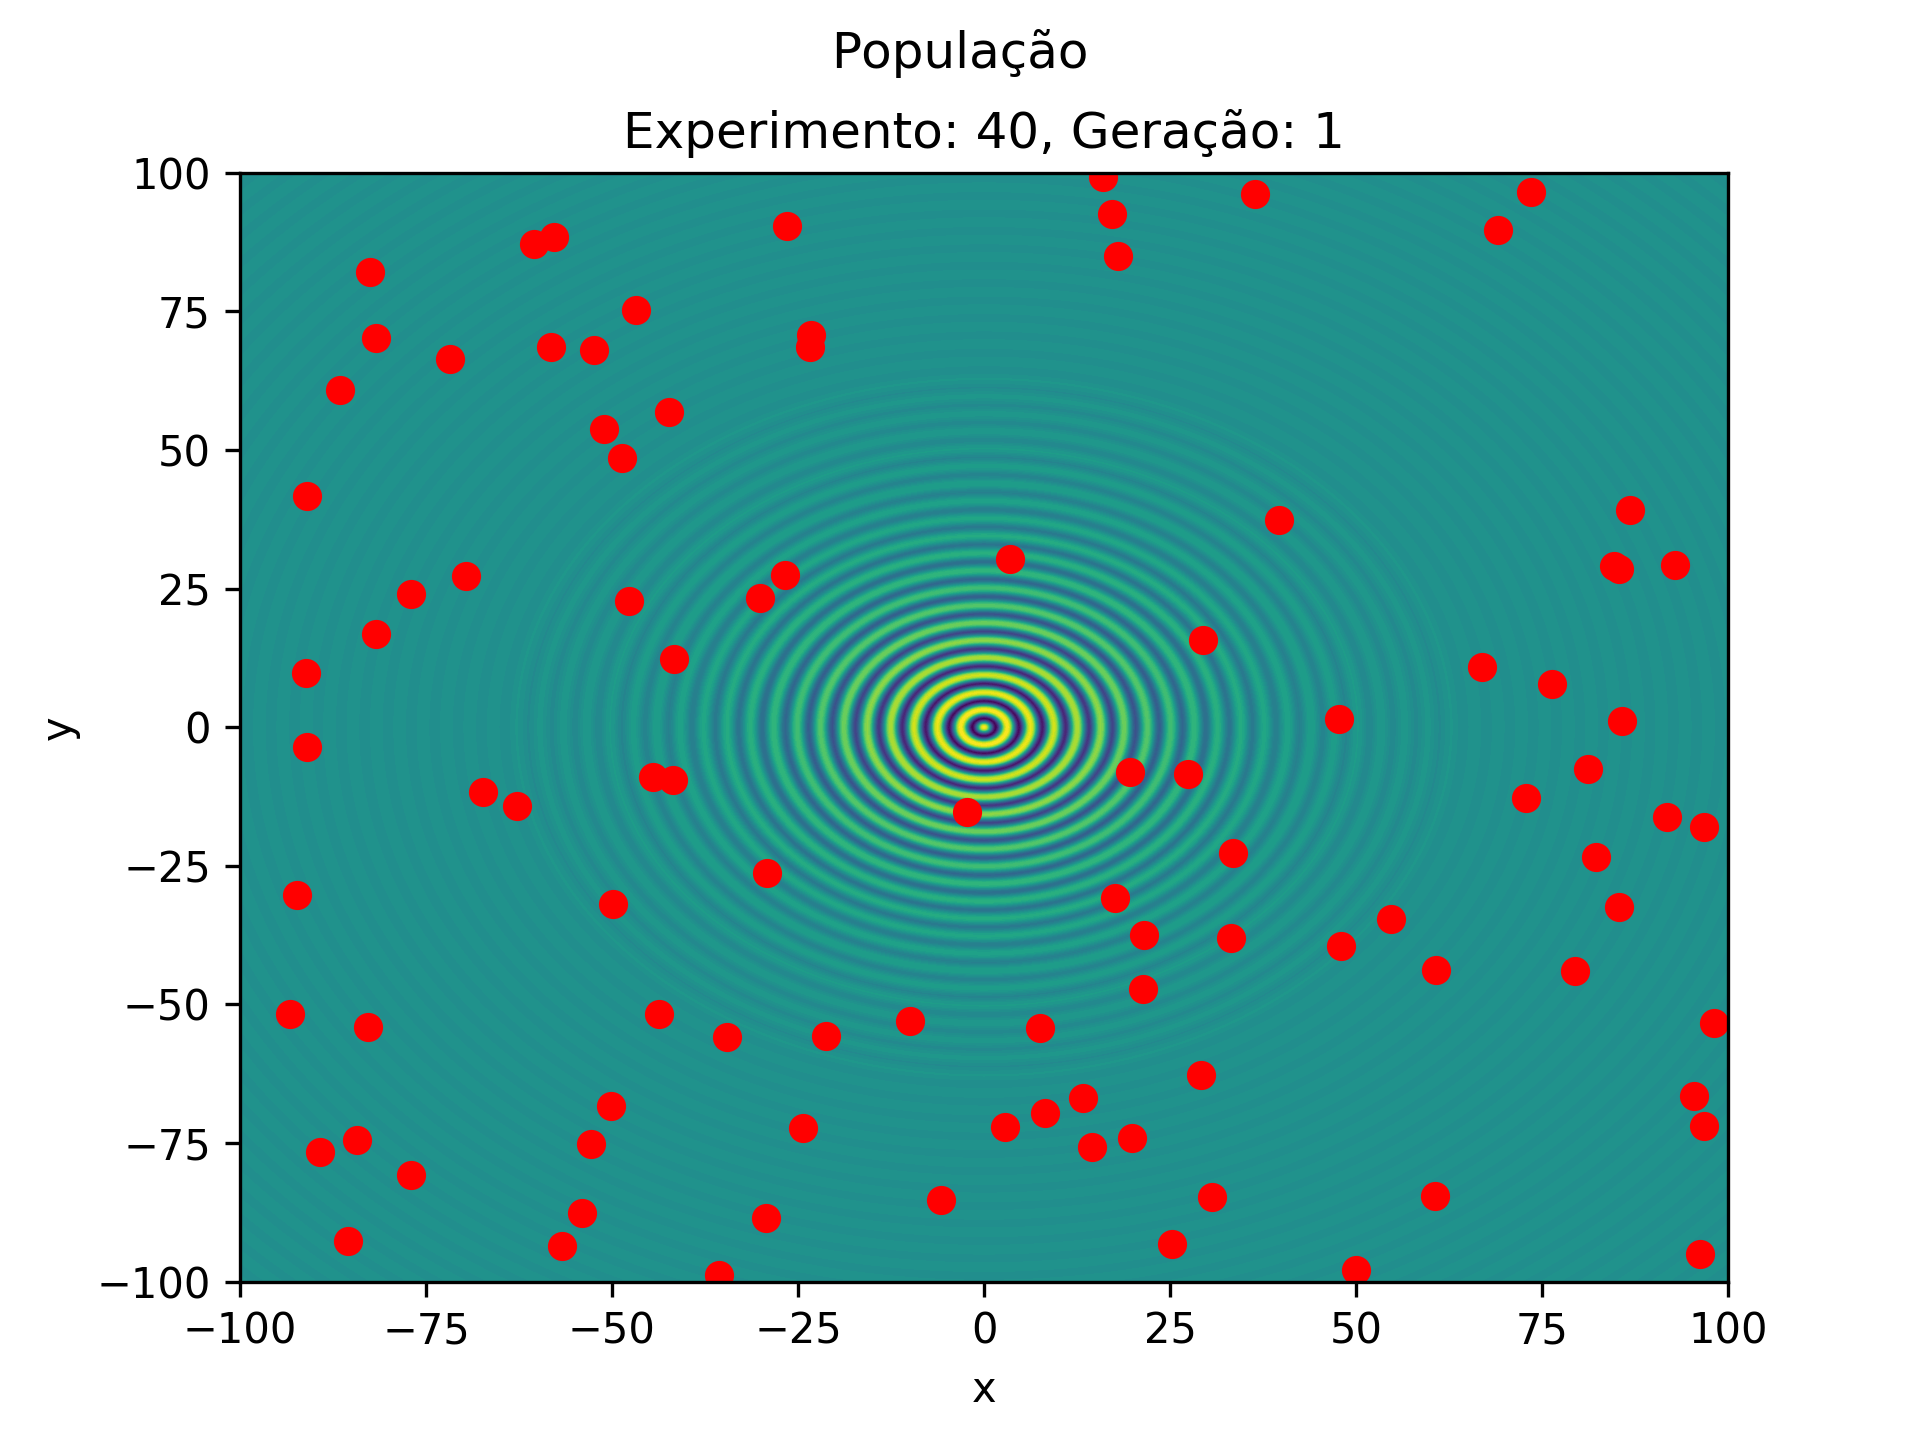
\includegraphics[width=0.9\linewidth]{sec-04/f6_population_gen_1_exp_40.png}
	  \end{subfigure}
	  \begin{subfigure}{.5\textwidth}
		\centering
		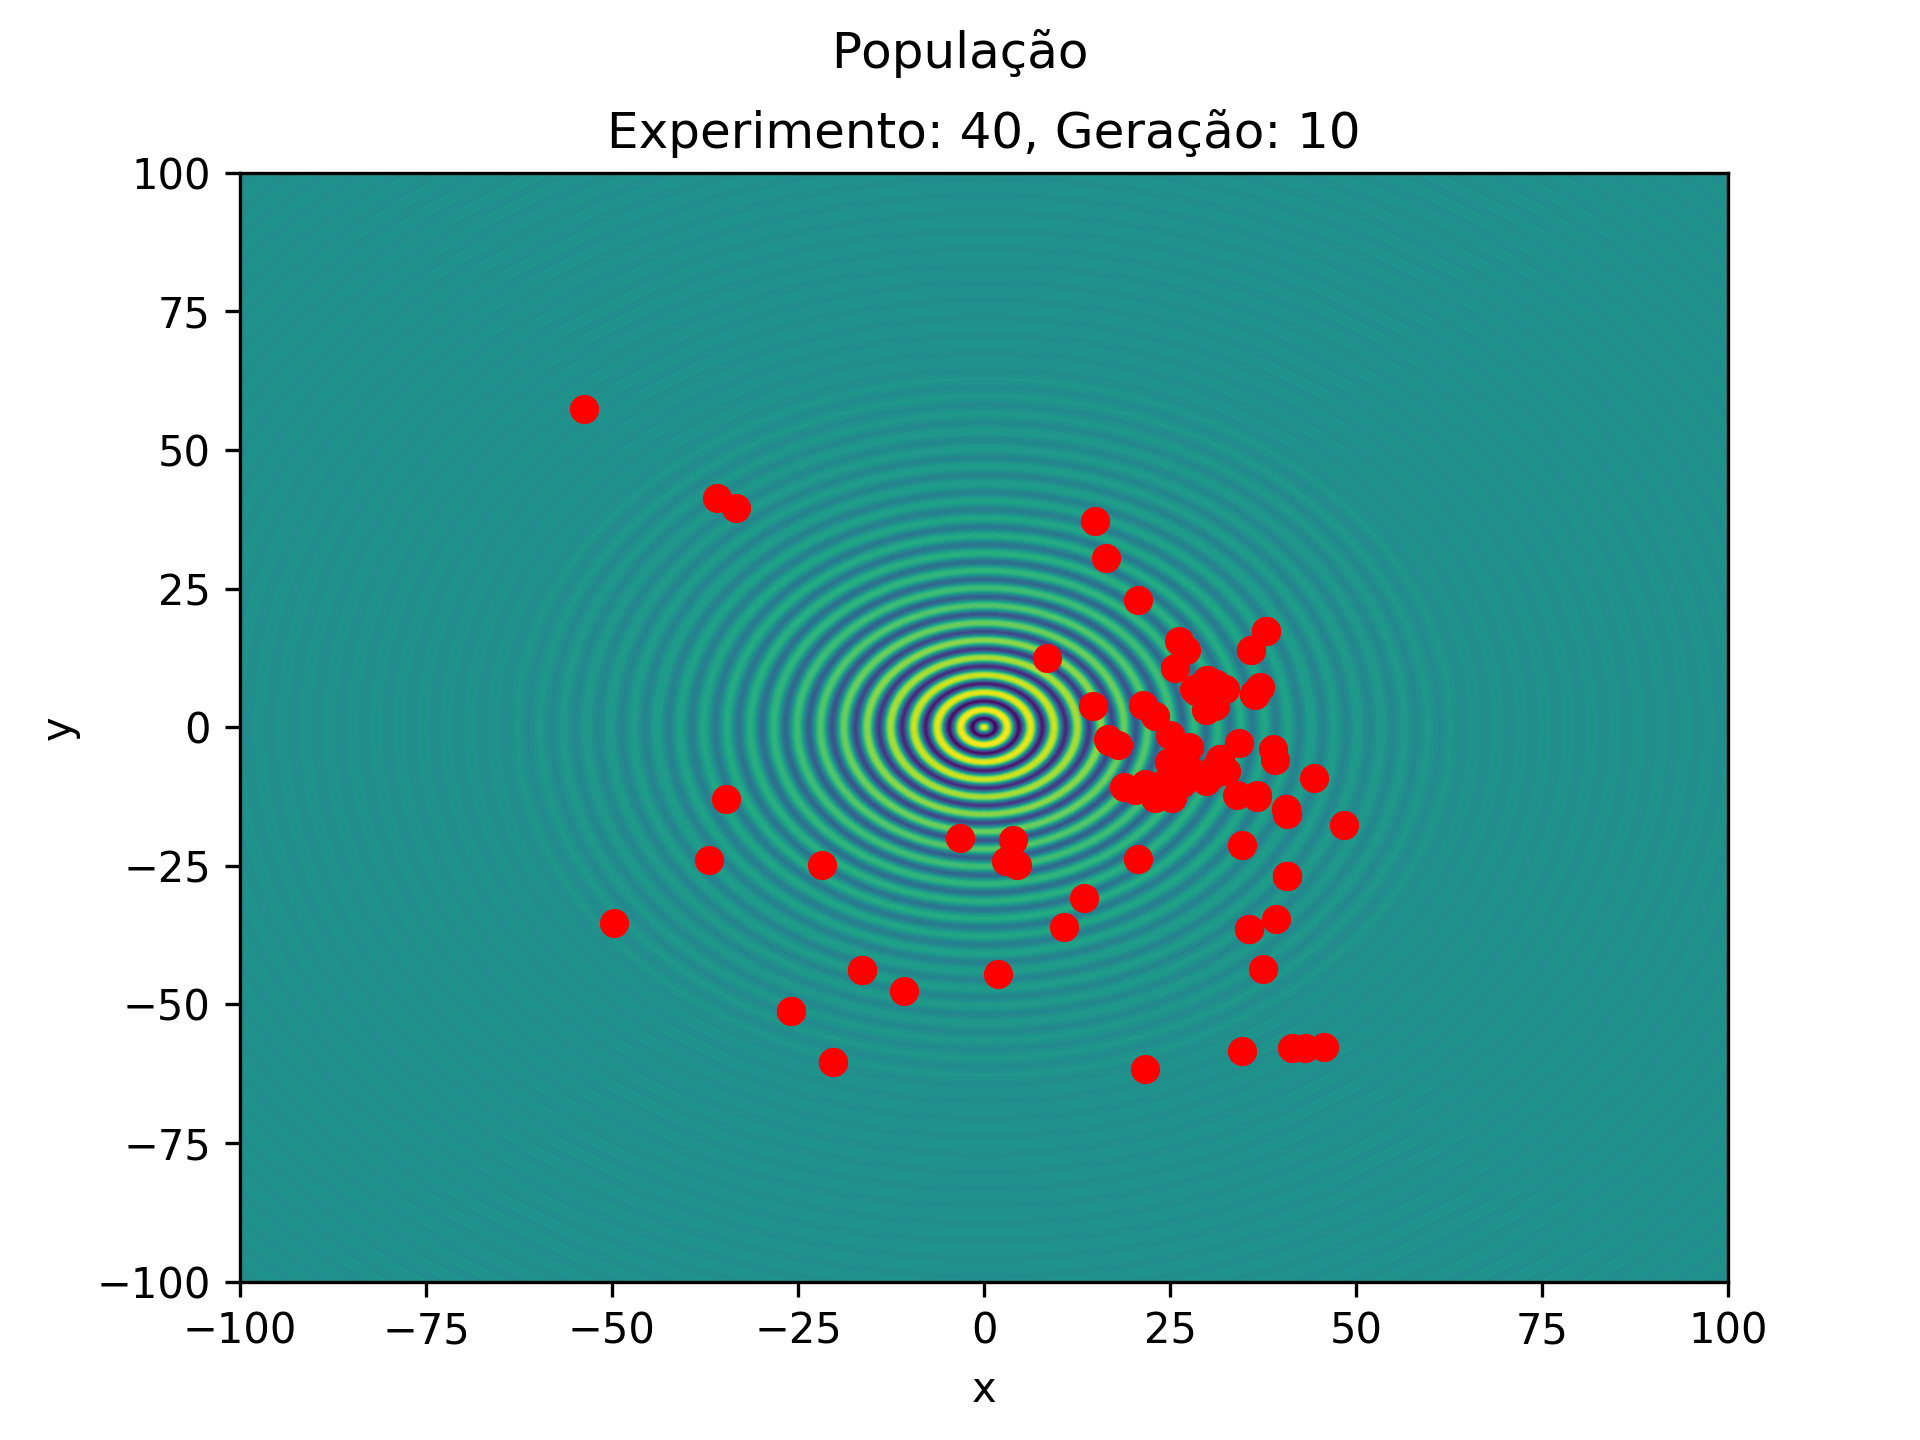
\includegraphics[width=0.9\linewidth]{sec-04/f6_population_gen_10_exp_40.png}
	  \end{subfigure}
	  \begin{subfigure}{.5\textwidth}
		\centering
		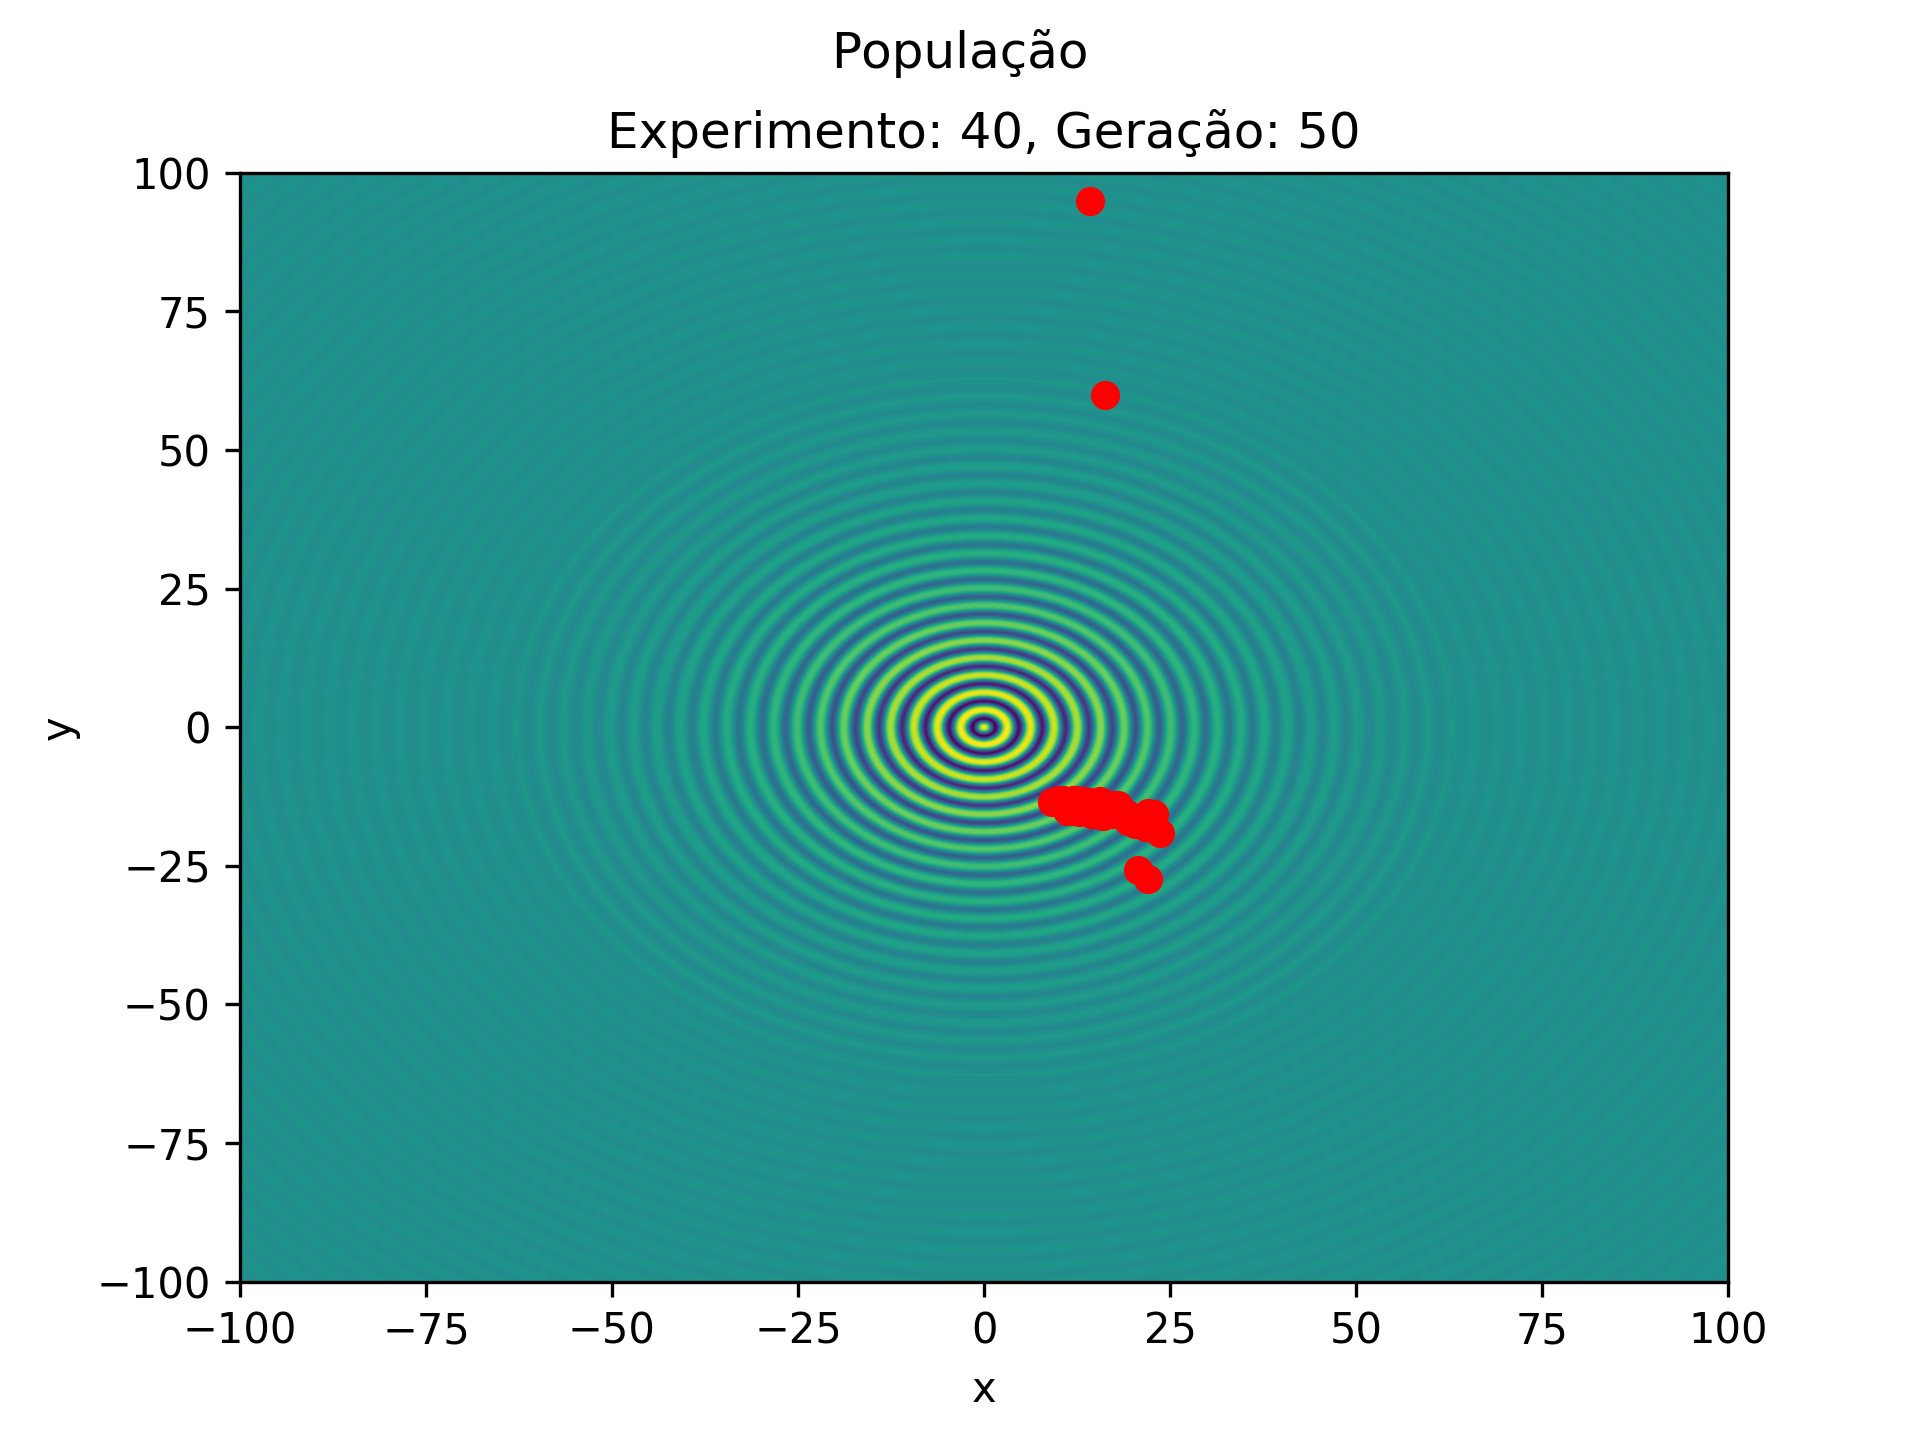
\includegraphics[width=0.9\linewidth]{sec-04/f6_population_gen_50_exp_40.png}
	  \end{subfigure}
	  \begin{subfigure}{.5\textwidth}
		\centering
		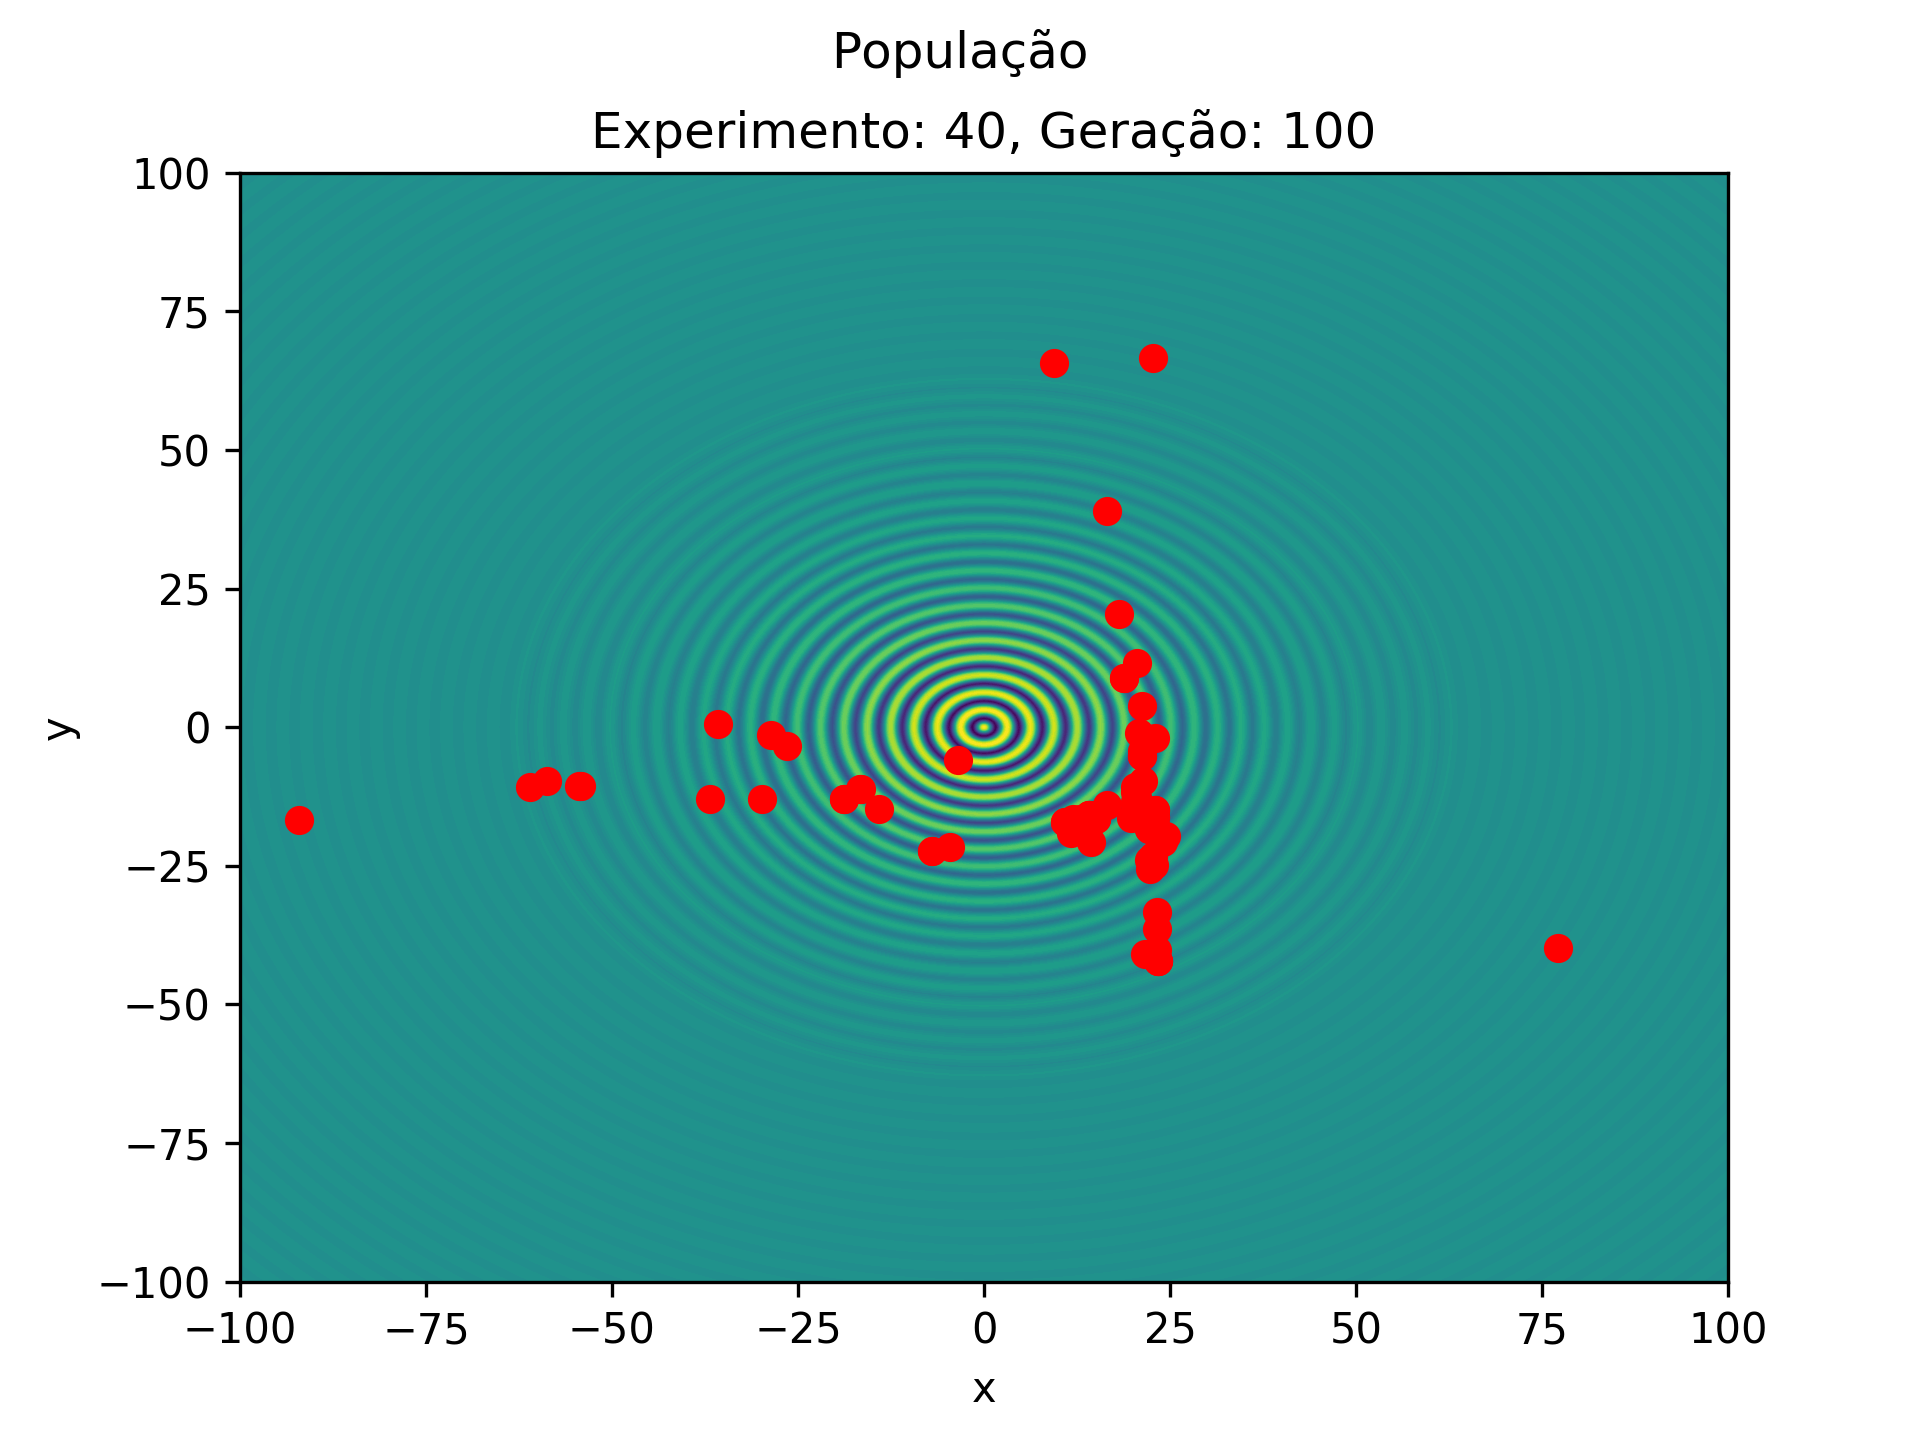
\includegraphics[width=0.9\linewidth]{sec-04/f6_population_gen_100_exp_40.png}
	  \end{subfigure}
	\caption{Populações do experimento 40 nas gerações 1, 10, 50 e 100.}
	\end{figure}

\end{document}
